%\documentclass[a4paper,12pt]{report}
\documentclass[a4paper,twoside,11pt]{report}
\usepackage[slovak,english]{babel}
\usepackage[T1]{fontenc}             
\usepackage[utf8]{inputenc}    
\usepackage{lmodern}
\usepackage{amsmath}
\usepackage{amssymb,amsfonts,amscd}
\usepackage{array,hhline}
\usepackage{makeidx}
\usepackage{fancyhdr}
\usepackage{graphicx}
\usepackage{listings}
    %%\usepackage{titlepage}
    %%\usepackage{multicol}
\usepackage{eurosym}
\usepackage{url,mathptmx} 
\usepackage[pdftex,unicode,bookmarks=false]{hyperref}

% Janechova sablona pouziva XeTEX - ale ked sa pouzije v tejto
% sablone, znaky s diakritikou sa nezobrazia spravne
%\usepackage[xetex,unicode,bookmarks=false]{hyperref}


%%%%%%%%%%%%%%%%%%%%%%%%%%%%%%%%%%%%%%%%%%%%%%%%
% Moje pridane balicky

% Celkovy pocet stran zaverecnej prace.
% Uzitocny v abstrakte
\usepackage{lastpage}

% Tabulka (aj) na uvodnej strane
\usepackage{tabu}

% Pouzite na tabulku "Porovnanie EVE-ng serverov",
% aby sa zvacsilo odsadenie od okrajov pri
% viacriadkovom popise
\usepackage{makecell}

% Velka tabulka na viac stran pre porovnavanie EVE-ng verzii
\usepackage{longtable}

% Spajanie buniek vertikalne
\usepackage{multirow}

% Oprava prikazov "cline" a "cmidrule" v tabulkach 
% v jazyku "slovak" a "czech" v usepackage babel
\usepackage{regexpatch}
\makeatletter
% Change the `-` delimiter to an active character
\xpatchparametertext\@@@cmidrule{-}{\cA-}{}{}
\xpatchparametertext\@cline{-}{\cA-}{}{}
\makeatother

% Cislovanie obrazkov a tabuliek plynule, 
% bez uvodneho cisla kapitoly
\usepackage{chngcntr}
\counterwithout{figure}{chapter}
\counterwithout{table}{chapter}


% Mensie rozostupy medzi prvkami v zoznamoch
% napr. pre zoznamy "itemize" a "enumerate"
\usepackage{enumitem}


% Ukazky zdrojovych kodov sa nerozdelia
% na viac stran, ale zostanu pohromade
% na jednej strane
\usepackage{fancyvrb}

% Viacriadkovy komentar
\usepackage{verbatim}

\usepackage{afterpage}

%%%%%%%%%%%%%%%%%%%%%%%%%%%%%%%%%%%%%%%%%%%%%%%%


\renewcommand{\baselinestretch}{1.5}  % pre zvascenie riadkovania

\addtolength{\oddsidemargin}{-.5cm}
\addtolength{\evensidemargin}{-2.9cm}   
\addtolength{\topmargin}{0cm}
\addtolength{\textheight}{0pt}
\addtolength{\textwidth}{2.cm}
\addtolength{\textheight}{2.cm}
\newlength{\verbcorr}
\setlength{\verbcorr}{0ex}

\graphicspath{{./obrazky/}}

\newcommand{\nazovpraceSK}{Sieťové virtualizačné nástroje a ich využitie vo vyučovacom procese KIS}
\newcommand{\nazovpraceEN}{Network virtualization tools and their use in the KIS learning process}

%%%%%%%%%%%%%%%%%%%%%%%%%%%%%%%%%%%%%%%%%%%%%%%%%

\begin{document}
\selectlanguage{slovak}

% Uvodne strany sa necisluju
% Cisluje sa az od obsahu
\pagestyle{empty}
\pagenumbering{arabic}      % Aktivujume cislovanie

\input{uvodne_strany/titulna_strana}

\newpage
\begin{titlepage}

\phantom.

\bigskip

\begin{center}
{\sc\LARGE Žilinská Univerzita v Žiline}

\medskip

{\sc\Large Fakulta riadenia a informatiky}

\vspace{4cm}

{\sc\LARGE Diplomová práca}

\medskip

{\large\bf \nazovpraceSK}

\bigskip

28360320182322

\end{center}

\phantom.\hfill
%\begin{minipage}{10cm}
\begin{center}


\begin{tabu} to 1.0 \textwidth { X[4,l] X[8,r] }
 Študijný odbor: & Aplikované sieťové inžinierstvo \\ 
 Katedra: & Katedra informačných sietí \\
 Vedúci diplomovej práce: & doc. Ing. Pavel Segeč, PhD. \\
\end{tabu}

\vspace*{\fill}

\begin{tabu} to 1.0 \textwidth { X[l] X[r] }
 Žilina 2018  & Bc. Andrej Šišila  \\
\end{tabu}

\end{center}
%\end{minipage}
\hspace{1.7cm}\phantom.

\vspace{2.9cm}

\phantom.
\end{titlepage}

\newpage
{\huge 1. STRANA ZADANIA DIPLOMOVEJ PRÁCE}

\newpage
{\huge 2. STRANA ZADANIA DIPLOMOVEJ PRÁCE}

\newpage
\input{uvodne_strany/podakovanie}

\newpage
\begin{abstract}

\noindent
{\sc Bc. Šišila Andrej:} {\em \nazovpraceSK} [Diplomová práca] 

\noindent
Žilinská Univerzita v Žiline, Fakulta riadenia a informatiky, Katedra informačných sietí.

\noindent  
Vedúci: doc. Ing. Pavel Segeč, PhD.
 
\noindent  
Stupeň odbornej kvalifikácie: Inžinier v odbore Aplikované sieťové inžinierstvo, Žilina. 

\noindent
FRI ŽU v Žiline, 2018 s. \pageref{LastPage}

\bigskip

Obsahom práce je nasadenie riešenia virtuálneho sieťového laboratória do vyučovacieho procesu na Katedre informačných sietí.

V prvej časti sa zaoberáme nástrojmi pre sieťovú virtualizáciu, ktoré následne porovnáme podľa zvolených kritérií, na základe ktorých vyberieme konkrétny nástroj. V druhej časti bude opísaná inštalácia vybraného nástroja a úpravy, ktoré rozširovali jeho funkcie a opravovali niektoré z jeho nedostatkov. Nakoniec je opísaný aj spôsob administrácie servera. Tretia časť je venovaná analýze vyučovaných tém pre vybrané predmety na Katedre informačných sietí. Štvrtá časť pojednáva o získavaní a testovaní virtuálnych zariadení. Na základe testovania sa vyberú vhodné zariadenia pre vyučované predmety.

V poslednej časti bude popísane nasadzovanie virtuálneho sieťového laboratória do vyučovacieho procesu pre konkrétne témy vyučované na vybraných predmetoch na Katedre informačných sietí.
\\
Kľúčové slová: virtualizácia, laboratórium, EVE-ng, Linux

\end{abstract}

\newpage
\selectlanguage{english}
\begin{abstract}

\noindent
{\sc Bc. Šišila Andrej:} {\em \nazovpraceEN} [Diploma thesis] 

\noindent
University of Žilina, Faculty of Management Science and Informatics, Department of information networks.
 
\noindent
Tutor:  doc. Ing. Pavel Segeč, PhD.
 
\noindent
Qualification level: Engineer in field Applied network engineering, Žilina: 

\noindent
FRI ŽU in Žilina, 2018 p. \pageref{LastPage}

\bigskip

The main idea of this thesis is the deployment of a virtual network laboratory into the learning process in the Department of information networks.

In the first part are analyzed the tools for network virtualization. These are compared according to chosen criteria, by which a specific solution is selected. In the second part is described the installation and adjustments of the selected tool which extended its functions and corrected some of its flaws. In the end is described the way of server administration. The third part says about the analysis of the learning topics for selected subjects in the Department of information networks. The fourth part explains the acquiring and testing of virtual devices. Based on the testing, appropriate devices for specific subjects are selected.

In the last part is described the deployment of the virtual network laboratory into the learning process for specific topics taught in chosen subjects in the Department of information networks.

Keywords: virtualization, laboratory, EVE-ng, Linux

\end{abstract}

\selectlanguage{slovak}

\newpage
\centerline{\bf Prehlásenie}

\vspace{2em}

\noindent
Prehlasujem, že som túto prácu napísal samostatne, a že som uviedol všetky použité pramene \\a literatúru, z ktorých som čerpal. 

\vspace{2em}

\noindent

V Žiline, dňa 2.5.2018

\hfill

Bc. Andrej Šišila

{\setlength{\parskip}{1pt plus 1pt}

\markboth{}{}

% newpage je nutny pre spravne cislovanie
\newpage

% Nastav spravne cislo strany
\setcounter{page}{8}

% Zobraz cislovanie v tejto casti
\pagestyle{plain}

\addcontentsline{toc}{chapter}{Obsah}
\tableofcontents

%\vspace{0pt plus 2cm}

\newpage
\addcontentsline{toc}{chapter}{Zoznam ilustrácii}
\listoffigures

%\vspace{0pt plus 2cm}

\newpage
\addcontentsline{toc}{chapter}{Zoznam tabuliek}
\listoftables

\newpage
\chapter*{Zoznam skratiek a značiek}
\addcontentsline{toc}{chapter}{Zoznam skratiek a značiek}

\begin{longtabu} to \textwidth {X[1.0,l] X[0.2,c] X[5,l]}
    \textbf{ACL} & - & Access list \\
    
    % BGP
    \textbf{BGP} & - & Border Gateway Protocol \\
    \textbf{eBGP} & - & external BGP \\
    \textbf{iBGP} & - & internal BGP \\
    \textbf{MP-BGP} & - & Multiprotocol BGP \\
    
    % VPN
    \textbf{VPN} & - & Virtual Private Circuit \\
    \textbf{EVPN} & - & Ethernet VPN\\
    \textbf{BGP mVPN} & - & BGP multicast VPN \\
    \textbf{BGP mVPN NG} & - & BGP mVPN Next Generation\\
    
    \textbf{BPDU} & - & Bridge Protocol Data Unit \\
    \textbf{BSR} & - & Bootstrap Router \\
    \textbf{CCIE} & - & Cisco Certified Internetwork Expert \\
    \textbf{CCNA} & - & Cisco Certified Network Associate \\
    \textbf{CCNP} & - & Cisco Certified Network Professional \\
    \textbf{CDP} & - & Cisco Discovery Protocol \\
    \textbf{CEF} & - & Cisco Express Forwarding \\
    \textbf{CLI} & - & Command Line Interface \\
    \textbf{CPU} & - & Central Processing Unit, Procesor \\
    \textbf{DHCP} & - & Dynamic Host Control Protocol \\
    \textbf{DMZ} & - & Demilitarized zone, Demilitarizovaná zóna \\
    \textbf{DTP} & - & Dynamic Trunking Protocol \\
    \textbf{EIGRP} & - & Enhanced Interior Gateway Routing Protocol \\
    \textbf{FHRP} & - & First Hop Redundancy Protocol \\
    \textbf{GLBP} & - & Gateway Load Balancing Protocol \\
    \textbf{GNS3} & - & Graphical Network Simulator 3 \\
    \textbf{GRE} & - & Generic Routing Encapsulation \\
    \textbf{HDLC} & - & High-Level Data Link Control \\
    \textbf{HSRP} & - & Hot Standby Router Protocol \\
    \textbf{IGMP} & - & Internet Group Management Protocol \\
    \textbf{IOL} & - & IOS on Linux \\
    \textbf{IOU} & - & IOS on Unix \\
    \textbf{IP SLA} & - & Internet Protocol Service Level Agreement \\
    \textbf{IS-IS} & - & Intermediate System to Intermediate System \\
    \textbf{ISL} & - & Inter-Switch Link \\
    \textbf{LACP} & - & Link Aggregation Control Protocol \\
    \textbf{LDP} & - & Label Distribution Protocol \\
    \textbf{LLDP} & - & Link Layer Discovery Protocol \\
    
    % PPP
    \textbf{PPP} & - & Point-to-Point Protocol \\
    \textbf{MLPPP} & - & Multilink PPP \\
    \textbf{PPPoE} & - & PPP over Ethernet \\
    
    \textbf{MLS} & - & Multilayer Switching / Multilayer Switch \\
    \textbf{MPLS} & - & Multiprotocol Label Switching \\
    \textbf{MST} & - & Multiple Spanning Tree \\
    \textbf{NAT} & - & Network Address Translation \\
    \textbf{NTP} & - & Network Time Protocol \\
    \textbf{OSPF} & - & Open Shortest Path First \\
    \textbf{PAGP} & - & Port Aggregation Protocol \\
    \textbf{PIM} & - & Protocol Independent Multicast \\
    
    % RIP
    \textbf{RIP} & - & Routing Information Protocol \\
    \textbf{RIPng} & - & RIP next generation \\
    
    \textbf{RP} & - & Rendezvous Point \\
    \textbf{RSVP} & - & Resource Reservation Protocol \\
    \textbf{SDN} & - & Software Defined Networking \\
    \textbf{SNMP} & - & Simple Network Management Protocol \\
    \textbf{SPAN} & - & Switch Port Analyzer \\
    
    % STP
    \textbf{STP} & - & Spanning Tree Protocol \\
    \textbf{PVST} & - & Per-VLAN Spanning Tree \\
    \textbf{RPVST} & - & Rapid PVST \\
    
    \textbf{SVI} & - & Switch Virtual Interface \\
    \textbf{UNL} & - & Unified Networking Laboratory, UNetLab \\
    \textbf{VIRL} & - & Virtual Internet Routing Lab \\
    
    % LAN
    \textbf{LAN} & - & Local Area Network \\
    \textbf{VLAN} & - & Virtual LAN \\
    \textbf{PVLAN} & - & Private VLAN \\
    \textbf{VPLS} & - & Virtual Private LAN Service \\
    \textbf{VTP} & - & VLAN Trunk Protocol \\
    
    \textbf{VRRP} & - & Virtual Router Redundancy Protocol \\
\end{longtabu}

% Nezapocitaj tabulku na zoznam skratiek
% a znaciek do zoznamu tabuliek
\addtocounter{table}{-1}
}

\markboth{}{}

\clearpage

%%%%%%%%%%%%%%%%%% obsah - koniec

%%%%%%%%%%%%%%%%%% kapitoly

% Zobraz cislovanie na vsetkych stranach,
% nie len na prvej strane kapitoly
\pagestyle{plain}

\chapter*{Úvod}
\addcontentsline{toc}{chapter}{Úvod}

Virtualizácia sa stáva vo svete čoraz populárnejšou. Využíva sa v rôznych oblastiach, napríklad v tzv. Cloud Computing alebo Software Defined Networking. Virtualizáciou sa zaberá aj Katedra informačných sietí Žilinskej univerzity v Žiline. Jedným z projektov, kde sa virtualizácia využíva, je projekt virtuálneho sieťového laboratória. 

Našou úlohou je preskúmať existujúce riešenia v oblasti virtuálnych sieťových laboratórii a porovnať ich podľa vopred stanovených kritérií (kapitola \ref{chap:nastroje_pre_siet_virt}). Na základe toho z nich vyberieme jedno riešenie, ktorým sa budeme v práci ďalej zaoberať. Pre vybrané sieťové laboratórium následne vypracujeme návody na inštaláciu, úpravu, používanie a nasadenie do infraštruktúry katedry (kapitola \ref{chap:eve_ng}). Následne si vyberieme predmety, na ktoré má byť tento nástroj použítý a analyzujeme technológie, ktoré sa na nich vyučujú. Zároveň odhadneme, ktoré zariadenia sú pre daný predmet vhodné (kapitola \ref{chap:analyza_vyucovania}). Potom analyzujeme kompatibilitu nástroja s rôznymi zariadeniami a vybrané zariadenia otestujeme podľa rôznych kritérii (kapitola \ref{chap:virt_zariadenia}). Nakoniec vybrané riešenie pre virtuálne sieťové laboratórium nasadíme do vyučovacieho procesu Katedry informačných sietí (kapitola \ref{chap:nasadenie_do_vyucovania}).

Virtuálne sieťové laboratórium bude nástrojom, ktorý zefektívni a skvalitní výučbu sieťových technológii vo vybraných predmetoch na Katedre informačných sietí.

Téma diplomovej práce bola vybraná predovšetkým preto, aby bol dosiahnutý kvalitnejší a efektívnejší vyučovací proces na katedre. Tak budú mať učitelia aj študenti jednotnú platformu pre vyučovanie, ktorá umožní jednoducho vytvárať modelové situácie pri riešení problémov v sieťovej infraštruktúre.
\chapter{Súčasný stav}

Je pomerne dobre známym faktom, že výučba nielen sieťových technológii je najúčinnejšia vtedy, keď má študent možnosť pracovať s vecami z reálneho sveta. Preto katedra disponuje fyzickými zariadeniami, ktoré pomáhajú študentom nabrať kvalitné skúsenosti. Avšak s fyzickými zariadeniami sa spájajú záväzky, ktoré nie je možné len tak ľahko prehliadnuť. Sú to napríklad:

\begin{enumerate}[noitemsep]
    \item Nedostatok prostriedkov na prevádzkovanie zariadení.
    \item Obmedzený prístup k zariadeniam. Ten je možný iba osobne v miestnosti špecializovanej na účel sieťového laboratória.
    \item Nedostatok priestoru pre fyzické zariadenia.
    \item Slabá miera izolácie pred prevádzkou generovanou v živej sieti.
    \item Postupná zastaranosť hardvéru alebo softvéru.
    \item Fyzické zariadenia sú náchylné na poruchy, čoho dôsledkom sú nesprávne fungujúce rozširujúce moduly alebo celé zariadenia. Tie treba buď opraviť, alebo vymeniť za nové. Následne treba myslieť na to, kam chybný hardvér umiestniť resp. ako ho odstrániť.
    \item Vyššia časová náročnosť pri prepájaní fyzických zariadení, predovšetkým pri náročnejších topológiách.
    \item So zvyšujúcim sa počtom zariadení v topológii rastie pravdepodobnosť, že ich študenti medzi sebou prepoja chybnými rozhraniami resp. sa pri prepájaní použije nesprávny typ kábla (použitie rovného Ethernet kábla namiesto kríženého a v.v.).
    \item Pomalšie spúšťanie a beh zariadenia, ktoré sú spôsobené načítaním operačného systému z pamäťovej karty a tým, že sieťové zariadenia sú špecializované na preposielanie rámcov a paketov, nie na rozbaľovanie komprimovaného súboru s operačným systémom.
    \item Náročné testovanie vzájomnej spolupráce zariadení. Ak by sme sa rozhodli vytvoriť topológiu so zariadeniami iných výrobcov, museli by sme si ich zaobstarať, čo vyžaduje ďalšie finančné a priestorové požiadavky.
\end{enumerate}

Vyššie uvedené problémy sa snažia riešiť rôzne virtualizačné platformy a nástroje, ktoré sú na nich postavené.

Vo svete pozorujeme trend rastúceho záujmu o virtuálne sieťové laboratóriá. Zo všetkých vymenujme dve univerzity, kde sa zaviedla táto forma výuky.

Na univerzite v \emph{Central University Taiwan} vytvorili v spolupráci s ďalšou univerzitou v Thajsku nástroj zvaný \emph{HVLab}, Hybrid Virtualization Laboratory. Ten v sebe integruje viacero prvkov. Používateľ pristupuje k topológii prostredníctvom webového rozhrania. Na serveri sa tieto topológie mapujú do GNS3 projektov. HVLab obsahuje aj tzv. logging, ktorý v reálnom čase zaznamenáva konfiguračné príkazy študenta a umožňuje učiteľovi vyhodnotiť jeho výkonnosť. Navyše nástroj obsahuje aj okno na výmenu správ v reálnom čase. Je rozdelené na skupinovú konverzáciu, ktorá má slúžiť na rýchlu výmenu konfigurácii medzi členmi tímu a súkromnú konverzáciu s učiteľom \cite{hvlab}. Nástroj je dostupný iba študentom na spomínanej univerzite.

Na \emph{Štátnej univerzite v Orenburgu} v Rusku sa skúmalo nasadenie ich vlastného návrhu virtuálneho sieťového laboratória na cloud platforme OpenNebula. Tak môžu poskytovať topológiu/infraštruktúru ako službu. Ich vlastný návrh riešenia spočíval v použití SDN návrhu v súčinnosti s nástrojmi Open vSwitch a OpenFlow. Topológie boli prístupné vo web rozhraní. Na grafickú interakciu s topológiou bol použitý komponent \emph{Draw2d touch}, ktorý umožňoval jednoduchú interaktivitu s prvkami topológie, ako napr. ich prepájanie čí presúvanie. Komponent na základe prepojení vygeneroval JSON súbor, ktorý topológiu definoval. Server pomocou tohto súboru vedel pracovať s topológiou a riadiť použité zdroje \cite{opennebula_lab}. Nástroj je dostupný iba pre študentov na spomínanej univerzite.

Tieto, a mnohé iné univerzity a školiace strediská si uvedomujú výhody virtualizácie sieťových prvkov a technológii pri vyučovaní.

Katedra sa tiež snaží držať krok so svetovým trendom. Aktívne sa na nej používajú viaceré riešenia virtualizovaného sieťového laboratória. Patria medzi ne Cisco Packet Tracer, Dynamips/Dynagen a GNS3.

Nástroj Cisco Packet Tracer sa momentálne používa na katedre pri vyučovaní kurzov CCNA Routing \& Switching, t.j. na predmetoch bakalárskeho stupňa štúdia Princípy informačno komunikačných technológii, Počítačové siete 1 a Počítačové siete 2.

Nástroj Dynamips/Dynagen sa používa pri výučbe predmetov bakalárskeho štúdia Počítačové siete 2, predmetov inžinierskeho štúdia Projektovanie sietí 1 a CCNP Routing (Pokročilé smerovanie v informačno-komunikačných sieťach).

Nástroj GNS3 sa na katedre používa lokálne, keďže ešte nie je dostatočne podrobne preskúmané nasadenie GNS3 ako vzdialený server. Slúži pre učiteľov na testovanie topológii a vyučovaných technológii nielen na predmetoch a kurzoch so zameraním na Cisco technológie, ale aj na testovanie spolupráce zariadení iných výrobcov, napr. spolupráca Cisco smerovačov s Juniper či Linux smerovačmi.

Katedra takisto disponuje aj nástrojom Cisco VIRL, ten sa však vo vyučovaní nepoužíva.

Katedre napriek tomu ešte stále chýba centralizované riešenie virtuálneho sieťového laboratória, ktoré by podporovalo všetky zariadenia spomenutých riešení. Túto situáciu sa v minulosti pokúšali niekoľkokrát zmeniť, pričom najbližšie sa zatiaľ dostal nástroj \emph{ViRo2} od Ing. Petra Hadača. Ten sa žiaľ pri vyučovaní používa veľmi zriedkavo.

Ďalšími vhodnými kandidátmi z prostredia open-source sú GNS3 a UNetLab, resp. EVE-ng. Hlavne GNS3 má už dlhoročnú tradíciu, narozdiel od už nevyvíjaného projektu UNetLab a jeho nasledovníka, EVE-ng. EVE-ng vyvíjala iná skupina vývojárov než UNetLab a dnes je už v štádiu, kedy dokáže robiť kvalitnú konkurenciu nástroju GNS3 a Cisco VIRL.

UNetLabv2, ktorý má byť tiež nasledovníkom projektu UNetLab, avšak z dielne pôvodného autora, žiaľ ešte nie je verejne prístupný, hoci sa na jeho vývoji pracuje.

Spomenuté nástroje sú podrobnejšie opísané v kapitole \ref{chap:nastroje_pre_siet_virt} - \nameref{chap:nastroje_pre_siet_virt}.
\chapter{Ciele práce}

Primárnym cieľom práce je nasadenie vhodného nástroja virtuálneho sieťového laboratória do vyučovacieho procesu katedry. Na naplnenie tohto cieľa bolo potrebné vykonať nasledovné úlohy:

\begin{itemize}[noitemsep]
    \item Prieskum existujúcich riešení pre virtuálne sieťové laboratórium a ich následné porovnanie na základe zvolených kritérií.
    \item Voľba konkrétneho riešenia pre virtuálne sieťové laboratórium, vyplývajúca z porovnania existujúcich riešení.
    \item Inštalácia nástroja virtuálneho laboratória infraštruktúry Katedry informačných sietí a jeho následná úprava pre potreby KIS.
    \item Výber predmetov, pre ktoré bude virtuálne laboratórium vhodné na použitie.
    \item Analýza vyučovaných tém na vybraných predmetoch.
    \item Testovanie zariadení pre beh vo virtuálnom sieťovom laboratóriu.
    \item Výber vhodných systémov sieťových zariadení pre konkrétne predmety na základe podporovaných technológii daného zariadenia.
    \item Overenie funkčnosti virtuálneho sieťového laboratória vo vyučovacom procese Katedry informačných sietí na konkrétnych predmetoch.
\end{itemize}
\chapter{Nástroje pre sieťovú virtualizáciu}
\label{chap:nastroje_pre_siet_virt}

V tejto kapitole uvádzam prehľad momentálne dostupných nástrojov virtuálnych sieťových laboratórií a ich porovnaniu na základe kritérií v časti \ref{chap:porovnavacie_kriteria} - \nameref{chap:porovnavacie_kriteria}.





\section{Porovnávacie kritériá}
\label{chap:porovnavacie_kriteria}

Pri porovnávaní jednotlivých virtuálnych sieťových laboratórii boli zohľadnené tieto kritériá:
\begin{itemize}[noitemsep]
    \item Použité vývojové technológie.
    \item Podpora zariadení.
    \item Typ používateľského rozhrania.
    \item Prideľovanie portových čísel zariadeniam.
    \item Vzdialený prístup ku zariadeniam.
    \item Vytvorenie/úprava/uloženie/odstránenie topológie.
    \item Počet topológii, ktoré môže mať jeden používateľ spustených.
    \item Možnosť práce viac ľudí naraz na rovnakom projekte.
    \item Možnosť prepojiť topológiu so živou sieťou.
    \item Podpora nástroja v budúcnosti.
    \item Vybrané výhody a nevýhody nástroja.
    \item Dokumentácia
\end{itemize}

V nasledujúcich častiach sú popísané jednotlivé riešenia virtuálneho sieťového laboratória.





\section{Cisco Packet Tracer}

Cisco Packet Tracer je nástroj na vizualizáciu sietí vyvíjaný spoločnosťou Cisco. Je vhodný na uvedenie do problematiky sieťových technológii. Slúži na emuláciu jednoduchých aktívnych aj pasívnych sieťových prvkov a jednoduchých koncových zariadení \cite{packet_tracer}. Čo sa týka smerovačov a prepínačov, sú emulované iba zariadenia od výrobcu Cisco a s obmedzenou funkcionalitou.

Nevýhodou je, že najnovšia verzia je prístupná výlučne pre členov \emph{Cisco Networking Academy}. K nevýhodám Cisco Packet Tracer tiež patrí, že nemá otvorený zdrojový kód čo znamená, že ho nie je možné ďalej rozširovať ani funkcionálne, ani pridávať podporu pre ďalšie zariadenia, napr. pre sieťové zariadenia iných výrobcov alebo koncové stanice Linux/Windows. 

Na druhej strane je vyvíjaný pre platformy Windows, Linux a Android, po emulácii aj na macOS \cite{packet_tracer_mac} a dokonca sú podporované aj mobilné platformy prostredníctvom aplikácie \emph{Packet Tracer Mobile}.

Nástroj Packet Tracer je možné používať výlučne lokálne, pretože pre tento nástroj neexistuje serverové riešenie. Vzdialený prístup, vytváranie a  topológii sa realizuje prostredníctvom grafického rozhrania aplikácie. Nástroj nevie rozlišovať rôzne typy používateľov. Je nenáročný na systémové zdroje. Umožňuje pracovať súčasne iba s jednou topológiou, pričom topológiu nie je možné prepojiť so živou sieťou.

Na obrázku \ref{obr:packet_tracer} je znázornené rozhranie nástroja Cisco Packet Tracer.

\begin{figure}
    \centering
    \includegraphics[width=0.65\textwidth]{packet_tracer}
    \caption{Nástroj Cisco Packet Tracer spustený v prostredí Windows}
    \cite{obr_packet_tracer}
    \label{obr:packet_tracer}
\end{figure}





\section{Dynamips/Dynagen}

Dynamips je emulátor Cisco smerovačov určený pre OS  Linux/Windows \cite{dynamips}. Nástroj v prevažnej miere napísaný v jazyku C a má otvorený zdrojový kód \cite{dynamips_github}. Podporuje výlučne vybrané typy Cisco smerovačov \cite{dynamips}. Ovláda sa cez príkazový riadok. Portové čísla pre vzdialený prístup na konzolu sa zariadeniam prideľujú manuálne. Vzdialený prístup k zariadeniam v topológii je realizovaný protokolom \emph{telnet}. Na vytváranie topológii sa používa jednoduchý značkovací jazyk \emph{NETMAP}.

Nástroj Dynagen tvorí nadstavbu pre platformu Dynamips a slúži na jednoduchšiu prácu s topológiami \cite{dynamips}. Topológie môže spravovať výlučne administrátor (alebo vlastník), pretože ani Dynamips, ani Dynagen nevedia rozlišovať rôzne typy používateľov. Počet topológii, ktoré môžu byť súčasne spustené je obmedzený iba výkonom servera. Na jednej topológii môžu pracovať aj viacerí študenti, tým že sa rozdelia portové čísla zariadení v topológii medzi študentov. Nástroj Dynamips umožňuje prepojiť topológiu so živou sieťou \cite{dynamips, dynamips_nil}.

V súčasnosti sa o nástroj Dynamips starajú vývojári nástroja GNS3 \cite{dynamips_github}. Na obrázku \ref{obr:dynamips_dynagen} je znázornený nástroj Dynagen.

\begin{figure}
    \centering
    \includegraphics[width=0.75\textwidth]{dynamips_dynagen}
    \caption{Nástroj Dynagen spustený v prostredí Windows} \cite{obr_dynamips_dynagen}
    \label{obr:dynamips_dynagen}
\end{figure}





\section{WEB-IOU (IOS on Unix)}

WEB-IOU, je simulačný nástroj pre platformu Linux, ktorý podporuje iba Cisco zariadenia na platforme IOU - IOS on Unix \cite{webiou_firewall_cx}. Jeho hlavnou výhodou je podpora Cisco prepínačov, ktorá v nástroji Dynamips/Dynagen chýba. Jeho autorom je Andrea Dainese \cite{webiou_github, webiou_unetlab_unetlabv2}. Nástroj je v prevažnej mierie napísaný v jazykoch PHP a JavaScript \cite{webiou_github}. Je vhodný na trénovanie pri certifikáciách CCNP a do istej miery aj CCIE.

Spravuje sa cez príkazový riadok. Používateľovi je dostupné web rozhranie. Portové čísla na vzdialený prístup sa zariadeniam prideľujú automaticky. Vzdialený prístup k zariadeniam v topológii je realizovaný protokolom \emph{telnet}. Na vytváranie topológii sa používa jednoduchý značkovací jazyk \emph{NETMAP}. Topológie môže spravovať ktokoľvek, kto má prístup k web rozhraniu, pretože ani tento nástroj nevie rozlišovať rôzne typy používateľov. Počet topológii, ktoré môžu byť súčasne spustené je obmedzený iba výkonom servera. Napriek tomu môžu na jednej topológii môžu pracovať aj viacerí študenti rovnakým spôsobom, ako pri nástroji Dynamips/Dynalab. Nástroj WEB-IOU umožňuje prepojiť topológiu so živou sieťou \cite{webiou_real_network}. 

V súčasnosti sa už nástroj nevyvíja. Na obrázku \ref{obr:webiou} je znázornené webové rozhranie nástroja WEB-IOU.

\begin{figure}
    \centering
    \includegraphics[width=0.75\textwidth]{webiou}
    \caption{Webové rozhranie nástroja WEB-IOU} \cite{obr_webiou}
    \label{obr:webiou}
\end{figure}





\section{Cisco VIRL}

Cisco VIRL, Virtual Internet Routing Lab, je komerčný simulačný nástroj sietí vyvíjaný spoločnosťou Cisco. Podporuje nielen Cisco smerovače a prepínače, ale aj zariadenia iných výrobcov. Nástroj je postavený na platforme Linux (Debian) a je dostupný ako virtuálny stroj pre rôzne platformy. Je vhodný na trénovanie pri certifikáciách CCNP a do istej miery aj CCIE \cite{virl_cisco}.

Výhodou oproti iným nástrojom je možnosť pridať do topológie vybrané podporované zariadenia, napr. koncové zariadenia, ako LXC kontajner \cite{virl_cisco}.

Nevýhodou je, že nepodporuje Dynamips/Dynagen emuláciu, takže na ňom nie je možné využiť existujúce virtuálne zariadenia na katedre \cite{virl_cisco}. Spomínaná integrácia zariadení iných výrobcov je síce možná, ale nemusí byť jednoduchá.

Spravuje sa cez príkazový riadok. Používateľovi je dostupné web rozhranie. Portové čísla na vzdialený prístup sa zariadeniam prideľujú automaticky \cite{virl_interfacett_1}. Vzdialený prístup k zariadeniam v topológii je realizovaný protokolmi \emph{telnet} a \emph{ssh}, po úprave aj \emph{vnc} \cite{virl_ciscoskills, virl_speaknetworks}. Na vytváranie topológii sa používa Nástroj \emph{VM Maestro}. Ten poskytuje možnosť, vopred si nakonfigurovať zariadenie podľa zvolených scenárov pomocou funkcie \emph{AutoNetkit}. Aj napriek tomu, že VIRL poskytuje pomerne široké možnosti na konfiguráciu Cisco zariadení a topológii, jeho používanie je pomerne obtiažne, hlavne pri vytváraní topológii \cite{virl_interfacett_1, virl_interfacett_2}. Cisco VIRL rozlišuje používateľov podľa typu na administrátorov a používateľov \cite{virl_cisco_features}. Počet topológii, ktoré môžu byť súčasne spustené je obmedzené iba výkonom servera. Napriek tomu môžu na jednej topológii pracovať aj viacerí študenti rovnakým spôsobom, ako pri nástroji Dynamips/Dynalab \cite{virl_interfacett_2}. Nástroj tiež umožňuje prepojiť topológiu so živou sieťou \cite{virl_speaknetworks}. 

Nástroj v súčasnosti existuje iba vo verzii \emph{Personal Edition} s licenciou na 20 zariadení, čo výrazným spôsobom obmedzuje jeho využitie vo vyučovaní. V minulosti existovali aj verzie \emph{Personal Edition} s licenciou na 30 zariadení a \emph{Academic Edition}. Rozdiel medzi Personal a Academic Edition bol iba ten, že Academic Edition bol prístupný učiteľom a študentom za výhodnejšiu cenu. Podporované funkcionality boli zhodné v oboch verziách \cite{virl_edition_differences}. Na obrázkoch \ref{obr:virl_vmmaestro} a \ref{obr:virl_web} je znázornený nástroj VM Maestro a webové rozhranie Cisco VIRL.

\begin{figure}
    \centering
    \includegraphics[width=0.75\textwidth,trim={0 0 5cm 0},clip]{virl_vmmaestro}
    \caption{VM Maestro} \cite{obr_virl_vmmaestro}
    \label{obr:virl_vmmaestro}

    \vspace{4cm}

    \centering
    \includegraphics[width=0.75\textwidth]{virl_web}
    \caption{Cisco VIRL web rozhranie} \cite{obr_virl_web}
    \label{obr:virl_web}
\end{figure}





\section{ViRo2}

ViRo2 je virtuálne laboratórium vytvorený na Katedre informačných sietí na Fakulte riadenia a informatiky Žilinskej univerzity v Žiline. Nástroj vznikol ako výsledok diplomovej práce Ing. Petra Hadača, pričom pokračoval v predchádzajúcej verzii nástroja ViRo. Nástroj je postavený na platforme Linux. Využíva technológie tzv. \emph{LAMP Stack} servera: Linux, Apache, MySQL, PHP (Drupal). Využíva virtualizáciu pomocou QEMU/KVM a Dynamips. Jeho hlavnou výhodou je možnosť rezervovať si topológiu. Ďalšou možnou nevýhodou je, že webové rozhranie stavia na platforme Drupal, ktorého popularita výrazne klesá \cite{stackoverflow_survey}. Okrem toho, takéto nástroje pre správu webovej stránky, ako napr. Wordpress, Joomla a.i. sa môžu stať potenciálnym bezpečnostným rizikom. \cite{incapsula_cms}

Spravuje sa prostredníctvom web rozhrania, SSH alebo VNC prístupu. Používateľom je dostupné webové rozhranie. Portové čísla na vzdialený prístup sa zariadeniam dajú nastaviť manuálne. Vzdialený prístup k zariadeniam v topológii je realizovaný viacerými spôsobmi: pomocou nástroja \emph{virsh}, aplikáciou \emph{Virtual Machine Manager} prístupnou cez \emph{vnc}, \emph{noVNC} serverom alebo SSH tunelom. Vytváranie topológii a správu zariadení sa používa grafický nástroj \emph{Virtual Machine Manager}. Nástroj ViRo2 vie rozlišovať používateľov s rolou \emph{administrátor}, \emph{učiteľ} a \emph{študent}. Topológie môže vytvárať iba používateľ s rolou \emph{učiteľ} alebo \emph{administrátor}. Počet topológii, ktoré môžu byť súčasne spustené je obmedzené iba výkonom servera. Napriek tomu môžu na jednej topológii môžu pracovať aj viacerí študenti rovnakým spôsobom, ako pri nástroji Dynamips/Dynalab. Nástroj umožňuje prepojiť topológiu so živou sieťou pomocou \emph{bridge} rozhrania \cite{viro_hadac}.





\section{UNetLab}

UNetLab, Unified Networking Lab, skrátene UNL, je open-source  simulačný nástroj pre platformu Linux, ktorý integruje všetky vyššie uvedené technológie na jednom mieste: Dynamips, Cisco IOU aj zariadenia tretích strán použitím QEMU/KVM technológie. Nástroj je postavený na platforme Linux. Jeho autorom je Andrea Dainese. V prevažnej mierie je napísaný v jazykoch PHP a JavaScript \cite{webiou_unetlab_unetlabv2, unetlab_github}. Je vhodný nielen na trénovanie pri Cisco certifikáciách, ale aj na testovanie vzájomnej spolupráce zariadení od rôznych výrobcov.

Spravuje sa cez príkazový riadok. Používateľovi je dostupné web rozhranie. Portové čísla na vzdialený prístup sa zariadeniam prideľujú automaticky. Vzdialený prístup k zariadeniam v topológii je realizovaný protokolom \emph{telnet} alebo \emph{vnc}. Topológie sa vytvárajú vo webovom rozhraní prepájaním uzlov medzi sebou pomocou myši, pričom sa na pozadí sa generuje súbor v značkovacom jazyku \emph{NETMAP}, ktorý o.i. definuje zariadenia v topológii. Topológie môže ktokoľvek, kto má prístup k web rozhraniu, pretože ani tento nástroj nevie rozlišovať rôzne typy používateľov, hoci v istej verzii nástroja táto funkcia bola podporovaná \cite{unetlab_github}. Počet topológii, ktoré môžu byť súčasne spustené je obmedzené iba výkonom servera. Napriek tomu môžu na jednej topológii môžu pracovať aj viacerí študenti rovnakým spôsobom, ako pri nástroji Dynamips/Dynalab. Jeden používateľ môže mať otvorenú práve jednu topológiu, ktorá sa dá zatvoriť až vtedy, keď v nej nie sú spustené žiadne zariadenia. Nástroj UNetLab tiež umožňuje prepojiť topológiu so živou sieťou pomocou \emph{bridge} rozhrania \cite{webiou_real_network}.

Vývoj tohto nástroja bol zastavený. UNetLab ďalej vyvíjala iná skupina vývojárov, ktorý nástroj premenovala na EVE-ng a migrovala ho z platformy Ubuntu 14.04 na Ubuntu 16.04. Jeho pôvodný autor následne začal s vývojom ďalšej verzie nástroja UNetLab, UNetLabv2, ktorému sa venujeme v časti \ref{chap:unetlabv2} - \nameref{chap:unetlabv2}. Na obrázku \ref{obr:unetlab_web} je znázornené webové rozhranie nástroja UNetLab.

\begin{figure}
    \centering
    \includegraphics[width=0.75\textwidth]{unetlab_web}
    \caption{Webové rozhranie nástroja UNetLab}
    \cite{obr_unetlab_web}
    \label{obr:unetlab_web}
\end{figure}





\section{EVE-ng}
\label{chap:virt_lab_eve_ng}

EVE-ng je simulačný nástroj sietí, ktorý vznikol ako klon a nasledovník nástroja UNetLab. Celkovou funkcionalitou, až na niektoré zmeny, napr. použitie MySQL namiesto SQLite, pridaná podpora pre ďalšie zariadenia), a vzhľadom webového rozhrania sa preto veľmi podobá na svojho predchodcu. Nástroj je postavený na platforme Linux a vyvíjaný prevažne v jazykoch JavaScript a PHP. Web rozhranie je realizované ako webová aplikácia s použitím framework nástroja \emph{Angular JS} a \emph{Twitter Bootstrap} \cite{eve_ng_technologies}.

EVE-ng sa v priebehu marca 2018 rozdelilo na tri verzie: Community, Professional a Learning Centre. Community verzia je open-source, aj keď \emph{gitlab} repozitár bol neprístupný pre verejnosť v priebehu novembra/decembra 2017. Napriek tomu sú na serveri všetky súbory prístupné a upravovateľné. Túto verziu je možné slobodne šíriť a upravovať. Verzia Professional obsahuje niektoré funkcionality, ktoré uľahčujú prácu s nástrojom, ale vývojári sa rozhodli spoplatniť ju. Learning Centre verzia obsahuje funkcionality na nasadenie do produkčného prostredia, ako je napr. rozdelenie používateľov do používateľských rolí. Podrobný zoznam podporovaných funkcii v jednotlivých verziách je dostupný v \cite{eve_ng_versions_table} a \cite{eve_ng_versions_list}.

Vzhľad webového rozhrania EVE-ng je znázornený na obrázku \ref{obr:eve_ng_web}. Rozdiely jednotlivých verzii EVE-ng sú znázornené v tabuľke \ref{tab:eve_ng_versions}.

\begin{figure}
    \centering
    \includegraphics[width=0.75\textwidth,trim={0 2cm 17cm 5cm},clip]{eve_ng_web}
    \caption{Webové rozhranie nástroja EVE-ng}
    \label{obr:eve_ng_web}
\end{figure}

Z tabuľky vyplýva, že verzia \emph{Community} je ako jediná bezplatná. Najväčšími výhodami ostatných verzii je rozdelenie používateľov do používateľských rolí a izolácia ich súborov (iba v \emph{Learning Centre}), zatvorenie topológie s už spustenými zariadeniami, prehľad zatvorených topológii so spustenými zariadeniami a zvýšený limit na počet spustených zariadení pre topológiu.

Doplnením a rozšírením funkcionality EVE-ng Community verzie je venovaná kapitola \ref{chap:eve_ng_uprava_zdroj_kodov} - \nameref{chap:eve_ng_uprava_zdroj_kodov}.

\newpage

\begin{longtable}{| m{3cm} | m{2cm} | m{2cm} | m{2cm} | m{4cm} |}
\caption{Porovnanie EVE-ng verzii}
\cite{eve_ng_versions_table}
\label{tab:eve_ng_versions} \\
\hline
Funkcia/Verzia                                      & Community         & Professional    & Learning Center      & Popis                                                                                                   \\ \hline
Cena                                                 & zadarmo              & 99 EUR  & 99 EUR & Pre Learning Center verziu platí, že pre každého ďalšieho používateľa, ktorý by sa chcel prihlásiť pod rovnakým používateľským menom, treba zaplatiť rovnakú sumu. Táto funkcia je vhodná pri spolupráci na rovnakej topológii.
\\ \hline
Používateľské role                                          & admin        & admin      & admin, user (študent), editor (učiteľ)  & Obmedzenia pre webových používateľov EVE-ng \\ \hline
Samostatný adresár pre každého používateľa                                  & Nie                & Nie              & Áno                  & Používateľ nemôže vidieť súbory a adresáre iného používateľa, iba svoje vlastné \\ \hline
Používateľ nemôže upravovať súbory                                 & Nie                & Nie              & Áno                  & Používateľ s rolou \emph{user} nemôže upravovať súbory ani prvky v topológii                                                                             \\ \hline
Adresár so zdieľanými topológiami                                     & Nie                & Nie              & Áno                  & Adresár so zdieľanými topológiami je viditeľný pre všetkých používateľov                                                                       \\ \hline
Platnosť používateľského účtu         & Nie                & Nie              & Áno                  & Možnosť nastaviť platnosť používateľského účtu v kalendári                         \\ \hline
Časomiera                                             & Nie                & Áno             & Áno                  & Do topológie je možné pridať časomieru na sledovanie trvania na vypracovanie                                                                                          \\ \hline
Adresár so spustenými topológiami                                   & Nie                & Áno             & Áno                  & Používatelia s rolou \emph{admin} a \emph{editor} môžu zatvoriť topológiu so spustenými zariadeniami a otvoriť ďalšiu topológiu. Topológie so spustenými zariadeniami sa objavia v osobitnom adresári.       \\ \hline
Node limit per lab                                    & 63                & 1024            & 1024                 & Limit of nodes to run per lab                                                                                 \\ \hline
Rozsah TCP portov                                             & pevný - 128 pre každého používateľa & dynamický - 1-65000 & dynamický - 1-65000      & Automatická voľba TCP portu na pre vzdialené pripojenie cez telnet                                     \\ \hline
Lokálne odchytávanie nástrojom Wireshark                               & Áno               & Nie              & Nie                   & Lokálne odchytávanie použitím SSH a \emph{root} používateľského účtu                          \\ \hline
Lokálny telnet klient                                   & Áno               & Áno             & Áno                  & Lokálny telnet klient musí byť nainštalovaný na počítači.                                                           \\ \hline
Lokálny VNC klient                                      & Áno               & Áno             & Áno                  & Lokálny VNC klient musí byť nainštalovaný na počítači.                                                              \\ \hline
Integrovaný nástroj Wireshark                                  & Nie                & Áno             & Áno                  & Nástroj Wireshark je integrovaný na serveri a je možné ho pridať do topológie na odchytávanie prevádzky. Pre verziu Community je dostupné iba odchytávanie pomocou lokálne nainštalovaného nástroja Wireshark.                                                                                   \\ \hline
Podpora Docker kontajnerov                              & Nie                & Áno             & Áno                  & Spúšťanie CLI aj grafických Docker kontajnerov.                                                                                      \\ \hline
Prepájanie už spustených zariadení (hot connections) & Nie                & Áno             & Áno                  & Pridávanie a odstraňovanie liniek medzi zariadeniami v topológii pre spustené zariadenia.                           \\ \hline
NAT Cloud                                             & Nie                & Áno             & Áno                  & Integrovaná NAT sieť umožňuje pripojiť zariadenia v topológii k internetu. Zariadeniam je následne pomocou DHCP pridelená IP adresa z rozsahu 169.254.254.0/24 \\ \hline
Desktop Console vo webovom rozhraní                                  & Nie                & Áno             & Áno                  & Integrovateľný Docker kontajner na správu koncových zariadení                          \\ \hline
Viacero spúšťacích konfigurácii pre topológiu            & Nie                & Áno             & Áno                  & Možnosť vytvárať a spúšťať topológie s rôznymi spúšťacími konfiguráciami pre jednotlivé zariadenia v topológii.                     \\ \hline
Exportovanie a importovanie konfigurácii z topológie     & Nie                & Áno             & Áno                  & Exportovanie a importovanie jednej alebo viacerých konfigurácii pre zariadenia v topológii na/z lokálny počítač                                             \\ \hline  
\end{longtable}





\section{GNS3}

GNS3, Graphical Network Simulator 3, je open-source sieťový simulátor sietí. Integruje všetky virtualizačné technológie najednom mieste: Dynamips, Cisco IOU aj zariadenia tretích strán (QEMU). Od verzie 1.5 sú v GNS3 podporované aj Docker kontajnery, čo je veľkou výhodou oproti iným nástrojom, pretože Docker kontajnery potrebujú menej systémových prostriedkov \cite{gns3_docker}.

GNS3 sa skladá z klientskej a serverovej časti. Klientská časť pozostáva z aplikácie \emph{GNS3 Client} a je celá napísaná v jazyku Python \cite{gns3_gui_github}. Klientská aplikácia je multiplatformová t.j. je kompatibilná s platformami Windows, Linux a macOS. Existuje aj klientská webová aplikácia \emph{gns3-web} \cite{gns3_web_github}. Tak by sa GNS3 priblížila k EVE-ng, keďže aj v EVE-ng sa používa webové rozhranie na prácu s topológiou.

Serverová časť môže byť realizovaná ako serverová aplikácia \emph{GNS3 Server}, ako virtuálny stroj \emph{GNS3 VM} alebo ako vzdialený server.

Serverová aplikácia \emph{GNS3 Server} sa spustí predvolene pri spustení klientskej aplikácie. Rovnako, ako GNS3 klientská aplikácia, aj serverová aplikácia je napísaná celá v jazyku Python \cite{gns3_server_github}.

GNS3 VM aj vzdialený server je postavený na platforme Linux. Vzdialený server nemusí nutne byť fyzický server, na ktorom je nasadený GNS3 server. Môže byť v ľubovoľnom virtualizačnom nástroji, ale odporúčaný je VMware, pretože podporuje vnorenú virtualizáciu, čo VirtualBox doposiaľ nepodporuje \cite{nested_virtualization}.

GNS3 VM, resp. vzdialený server, sa spravuje cez príkazový riadok. Používateľovi je dostupná klientská aplikácia. Portové čísla na vzdialený prístup sa zariadeniam prideľujú automaticky, avšak je možné manuálne meniť rozsah, v akom sa majú portové čísla automaticky prideľovať, dokonca umožňuje aj manuálnu zmenu čísla portu pre jednotlivé zariadenia \cite{gns3_console_ports, gns3_console_ports_remote}. Vzdialený prístup k zariadeniam v topológii je realizovaný protokolom \emph{telnet}, \emph{vnc} alebo \emph{rdp}. Topológie sa vytvárajú v klientskej aplikácii prepájaním uzlov medzi sebou pomocou myši. V predvolenom nastavení sú všetky topológie na GNS3 VM / vzdialenom serveri zdieľané a môže ich meniť ktokoľvek, kto má k serveru z GNS3 klientskej aplikácie, pretože v predvolenom nastavení nástroj nevie rozlišovať rôzne typy používateľov ani ich izolovať. Počet topológii, ktoré môžu byť súčasne spustené je obmedzené iba výkonom servera. Napriek tomu môžu na jednej topológii môžu pracovať aj viacerí študenti tým, že si otvoria rovnaký projekt na vzdialenom serveri. Zmeny v takejto zdieľanej topológii sa prejavia okamžite všetkým používateľom, ktorí majú túto topológiu práve otvorenú. Jeden používateľ môže mať spustených aj viacero topológii, klientská aplikácia však dovoľuje pracovať iba s jednou naraz. Aj GNS3, podobne ako aj ďalšie nástroje, umožňuje prepojiť topológiu so živou sieťou pomocou \emph{bridge} rozhrania alebo \emph{NAT} siete.

Vývoj tohto nástroja stále pokračuje. Na obrázku \ref{obr:gns3_client} je znázornená klientská aplikácia GNS3 Client.

\begin{figure}
    \centering
    \includegraphics[width=0.75\textwidth]{gns3_client}
    \caption{Klientská aplikácia GNS3}
    \label{obr:gns3_client}
\end{figure}





\section{UNetLabv2}
\label{chap:unetlabv2}

UNetLabv2 je nasledovníkom nástroja UNetLab. Je postavený na platforme Docker kontajnerov. Jednotlivé úlohy sú distribuované naprieč kontajnermi. To zaisťuje lepšiu škálovateľnosť pri zachovaní rovnakej funkcionality. Zatiaľ ešte nie je verejne nedostupný. \cite{webiou_unetlab_unetlabv2}

Architektúra nástroja UNetLabv2 je znázornená na obrázku \ref{obr:unetlabv2_arch}

\begin{figure}
    \centering
    \includegraphics[width=0.8\textwidth]{unetlabv2_arch}
    \caption{Architektúra nástroja UNetLabv2} \cite{obr_unetlabv2_arch}
    \label{obr:unetlabv2_arch}
\end{figure}





\section{Vyhodnotenie}

Z vyššie uvedených nástrojov má zmysel zaoberať sa nástrojmi EVE-ng a GNS3 z nasledovných dôvodov:
\begin{itemize}[noitemsep]
    \item Open-source vývoj oboch nástrojov umožňuje ich používanie bez poplatkov, obáv o porušenie licenčných podmienok a poskytuje možnosť upravovať ich podľa vlastných požiadaviek.
    \item Podpora rôznych virtualizačných technológii.
    \item Podpora zariadení od rôznych výrobcov.
    \item Jednoduché ovládanie.
\end{itemize}

V priebehu projektu sme sa preto zamerali na nástroje GNS3 a EVE-ng. Počas neho sa však ukázalo, že GNS3 nie je vhodná pre vzdialené použitie, preto sme sa týmto nástrojom ďalej nezaoberali. V čase skúmania bol nástroj GNS3 vo verzii 1.5.3. Keď sme skúšali použiť GNS3 ako vzdialený server, klientská aplikácia sa na GNS3 vzdialený server nevedela pripojiť, hoci sme postupovali podľa návodov na GNS3 stránke a pri testovaní nestála v pripojení na server žiadna prekážka, ako napr. firewall.

Napriek tomu je GNS3 silným nástrojom, schopným konkurovať EVE-ng. V tabuľke \ref{tab:gns3_eve_ng_porovnanie} porovnávame jednotlivé výhody a nevýhody oboch nástrojov.

% Please add the following required packages to your document preamble:
% \usepackage{multirow}
% \usepackage{longtable}
% Note: It may be necessary to compile the document several times to get a multi-page table to line up properly
\begin{longtabu} to \textwidth {| X[0.5,lm] | X[1.0,lm] | X[1.0,lm] |}
\caption{Porovnanie GNS3 a EVE-ng}
\label{tab:gns3_eve_ng_porovnanie} \\
\cline{2-3}
\multicolumn{1}{c}{} & \multicolumn{1}{|c}{\textbf{GNS3}}    & \multicolumn{1}{|c|}{\textbf{EVE-ng}}    \\ \hline
\endfirsthead
%
\endhead
%
\makecell[cc]{\multirow{8}{*}[-3cm]{\textbf{Výhody}}}   & \multicolumn{2}{c|}{Možnosť nasadenia ako vzdialené servery}                                                                                                                                                                                                                                                                                                                                                                                                                       \\ \cline{2-3} 
                                   & \multicolumn{2}{c|}{Podpora viacerých používateľov (multi-user)}                                                                                                                                                                                                                                                                                                                                                                                                                  \\ \cline{2-3} 
                                   & \multicolumn{2}{c|}{\makecell{Eventuálne možný import používateľských účtov na server z LDAP: \\ -pre GNS3 do operačného systému \\
                                   -pre EVE-ng do Linuxu alebo MySQL databázy}}                                                                                                                                                                                                                                                                                                                    \\ \cline{2-3}
                                   & \makecell[lc]{Multiplatformová klientská \\aplikacia (Windows/Linux/macOS)}                                                                                                                                                                                       & Multiplatformový klient - webová aplikácia                                                                                                                                                                                      \\ \cline{2-3} 
                                   & Natívna podpora Docker kontajnerov                                                                                                                                                                                                             & \makecell[lc]{Podpora Telnet/VNC vzdialeného\\ pripojenia ku zariadeniam cez\\ HTML5 reverse proxy server\\ (Apache Guacamole) - na\\ klientský počítač netreba\\ inštalovať  nič, okrem webového\\ prehliadača a nástroja Wireshark}                      
                                   
                                   \\ \cline{2-3} 
                                   
                                   & \makecell[lc]{Podpora viacerých používateľov\\ pri práci na spoločnom projekte\\ - pri práci viacerých používateľov\\ na jednom projekte sa topológia\\ sa pri zmene okamžite aktualizuje\\ všetkým používateľom a všetci\\ môžu pracovať so zariadeniami z\\ GNS3 klienta}
                                   
                                   & Podpora viacerých používateľov pri práci na spoločnom projekte - topológia sa aktualizuje až po kliknutí na \emph{Refresh topology}, nie okamžite po jej zmene                                                                       \\ \cline{2-3} 
                                   & \makecell[lc]{Lepšia škálovateľnosť oproti \\EVE-ng - možnosť vytvoriť\\ GNS3 cluster}                                                                                                                                                                             & Podpora viacerých používateľov - autentifikácia používateľa menom a heslom                                                                                                                                                      \\ \cline{2-3} 
                                   & \makecell[lc]{Širšie možnosti nastavenia \\z GNS3 klienta} & Užšie možnosti nastavenia z EVE-ng webového rozhrania.                                                                                                                                                                                                                                 \\ \hline
\makecell[cc]{\multirow{7}{*}[-4cm]{\textbf{Nevýhody}}} & \makecell[lc]{Nutnosť inštalácie samostatnej \\ klientskej aplikacie}                                                                                                                                                                                            & Pomalé HTML5 webové rozhranie                                                                                                                                                                                                   \\ \cline{2-3} 
                                   & Zložitejšia konfigurácia autentifikácie a izolácie používateľov                                                                                                                                                                                & \makecell[lc]{V Community verzii sú\\ používatelia sú typu \emph{administrátor}\\ a nie sú nijako od seba izolovaní -\\ ktokoľvek zaregistrovaný môže\\ pridávať/upravovať/odstraňovať \\projekty a adresáre používateľov \\(ošetrené v Learning Centre verzii)}                             \\ \cline{2-3} 
                                   & Zložitejšie vytváranie šablón pre zariadenia                                                                                                                                                                                                   & \makecell[lc]{Pri práci viacerých ľudí na\\ spoločnom projekte môže z\\ webovej aplikácie pristupovať k\\ zariadeniam iba jeden človek,\\ ostatní musia k zariadeniam\\ pristupovať pomocou IP adresy a\\ portu}                                           \\ \cline{2-3} 
                                   & Nutnosť manuálne pridať každé zariadenie do GNS3 klienta                                                                                                                                                                                       & Nutnosť vypnutia zariadenia, keď je potrebné pridať/odstrániť prepojenie s iným zariadením (ošetrené v Pro a Learning Centre verzii)                                                                                            \\ \cline{2-3} 
                                   & Pri nasadení GNS3 na viacero serverov (cluster) treba každé zariadenie pridať samostatne na každý server                                                                                                                                       & \makecell[lc]{V Community verzii Docker\\ kontajnery nie sú podporované.\\ Oficiálna podpora Docker\\ kontajnerov vrátane grafických je\\ prítomná iba vo verziách Pro a\\ Learning Centre; vo verzii\\ Community je experimentálna je\\ nutné ju aktivovať dodatočne}                                         \\ \cline{2-3} 
                                   & \makecell[lc]{Verzia klientskej aplikácie a\\ servera musia byť zhodné t.j.\\ musia sa naraz aktualizovať aj\\ klienstká, aj serverová časť, inak\\ nie je možné nástroj používať}                                                                                    & Web server Apache nie je chránený modulmi \emph{modsecurity} (ochrana napr. Proti SQL Injection) a \emph{modevasive} (ochrana proti DoS a DDoS útokom)                                                                                    \\ \cline{2-3} 
                                   &                                                                                                                                                                                                                                                & \makecell[lc]{EVE-ng sa nedá škálovať naprieč \\ viacerými servermi t.j. nevieme \\ urobiť EVE-ng cluster tak, \\ ako to je to možné v GNS3}                                                                                                           \\ \hline
\end{longtabu}

GNS3 od vydania stabilnej verzie 2.0.0 opravila problém s nasadením ako vzdialený server. Avšak vtedy som už začal s hlbším skúmaním EVE-ng. Skúmanie dvoch nástrojov naraz do hĺbky by bolo časovo veľmi náročné. GNS3 slúžila počas skúmania ako podporný nástroj pre pochopenie rôznych technických súčastí virtualizácie sieťových zariadení.

Vo zvyšku diplomovej práce sa zaoberám nástrojom \emph{EVE-ng Community Edition} a jeho nasadením do vyučovania na katedre.

\chapter{EVE-ng}
\label{chap:eve_ng}

EVE-ng je virtuálne sieťové laboratórium skladajúcej sa zo serverovej časti postavenej na platforme Linux a klientskej časti, ktorú tvorí webová aplikácia, ako je už spomenuté v kapitole \ref{chap:virt_lab_eve_ng}.

Serverová časť je realizovaná ako tzv. LAMP server, podobne ako nástroj ViRo2. LAMP je skratka pre \emph{Linux Apache MySQL PHP}. Webový server Apache poskytuje webovú stránku. MySQL je relačná databáza ukladajúca informácie o používateľoch webového rozhrania EVE-ng. Správe používateľských účtov sa venuje kapitola \ref{chap:sprava_pouzivatelov}. PHP je použitý na spracovanie REST API volaní z webového rozhrania. Webové rozhranie je vytvorené pomocou nástrojov \emph{Twitter Bootstrap v3.3.6} a \emph{AngularJS v1.5.6}.

V tejto kapitole bude opísaný proces nasadzovania EVE-ng servera do sieťovej infraštruktúry katedry: jeho inštalácie, následnej úpravy a základnej administrácie EVE-ng servera. Všetky kroky sú podrobne opísané v adresári s návodmi pre EVE-ng v kapitole \ref{chap:cd} v bode \ref{item:prilohy_cd_eve_ng_adresar}.





\section{Inštalácia}
\label{chap:eve_ng_instalacia}

EVE-ng bol inštalovaný a testovaný na dvoch platformách:

\begin{itemize}[noitemsep]
    \item VMware Workstation Player
    \item Fyzický server
\end{itemize}

Parametre VMware virtuálneho stroja a fyzického servera sú uvedené v tabuľke \ref{tab:server_parameters}. V oboch prípadoch bol EVE-ng server nasadený do DMZ zóny, preto v riadku \emph{IP adresa} uvádzam len posledný oktet ich IPv4 adries, keďže adresný rozsah DMZ zóny je na katedre známy.

\begin{longtabu} to \textwidth {| X[5.0,cm] | X[5.0,cm] | X[5.0,cm] |}
\caption{Parametre EVE-ng serverov}
\label{tab:server_parameters} \\
\hline
    \textbf{Parametre \textbackslash~ Server} & \textbf{VMware} & \textbf{Fyzický server} \\
\hline
    \textbf{CPU} & 16 & 8 \\
\hline
    \textbf{Operačná pamäť (GB)} & 64 & 48 \\
\hline
    \textbf{EVE-ng verzia} & 2.0.3-80 & 2.0.3-86 \\
\hline
    \textbf{IP adresa} & .49 & .50 \\
\hline
\end{longtabu}

\noindent
Uvedené tvrdenia platia pre EVE-ng vo vydaní \emph{Community Edition} vo verzii 2.0.3-86.

\noindent
Postup inštalácie EVE-ng servera môžeme zhrnúť do týchto krokov:

\begin{enumerate}[noitemsep]
    \item Vytvorenie vzdialenej pracovnej plochy a VMware Workstation (kap. \ref{chap:cd}, body \ref{item:vnc1}-\ref{item:vmware_extra_instalacia})
    \item Inštalácia Ubuntu Server 16.03.4 LTS (kap. \ref{chap:cd}, body \ref{item:instalacia_ubuntu_a_eve_ng}, \ref{item:aktualizacia_eve_ng})
    \item Konfigurácia Ubuntu Server (kap. \ref{chap:cd}, bod \ref{item:instalacia_ubuntu_a_eve_ng})
    \item Inštalácia EVE-ng do Ubuntu Server (kap. \ref{chap:cd}, bod \ref{item:instalacia_A_konfiguracia_eve_ng})
    \item Konfigurácia EVE-ng servera
\end{enumerate}

\noindent   
Konfigurácia EVE-ng servera zahŕňala:

\begin{enumerate}[noitemsep]
    \item Obnovenie súborov a adresárov (kap. \ref{chap:cd}, bod \ref{item:obnova_zalohovanie})
    \begin{itemize}[noitemsep]
        \item Skripty (kap. \ref{chap:cd}, bod \ref{item:skripty})
        \item Zariadenia (kap. \ref{chap:cd}, body \ref{item:pridavanie_konverzia_zariadeni}-\ref{item:pridavanie_win})
        \item Databázy (kap. \ref{chap:cd}, bod \ref{item:obnova_zalohovanie})
    \end{itemize}
    \item Automatizácia zálohovania (kap. \ref{chap:cd}, bod \ref{item:obnova_zalohovanie})
    \item Pridanie Cisco IOL/IOU licencie (kap. \ref{chap:cd}, bod \ref{item:iou_licencia})
    \item Zabezpečenie servera (kap. \ref{chap:cd}, bod \ref{item:zabezpecenie})
    \begin{itemize}[noitemsep]
        \item Systém
        \item SSH
        \item Webový server
    \end{itemize}
    \item Úprava šablón (kap. \ref{chap:cd}, bod \ref{item:uprava_sablon})
    \item Úprava zdrojových kódov (kap. \ref{chap:cd}, body \ref{item:spristupnenie_pouzivatelskych_roli}-\ref{item:zatvorenie_topologie_so_spustenymi_zariadeniami})
\end{enumerate}

Inštalačný proces pre obe platformy, virtuálnu aj fyzickú, bol takmer zhodný, líšil sa iba v úvodných krokoch. Pri inštalácii pre VMware bolo totiž potrebné na server, na ktorom bol VMware nainštalovaný, pridať VNC prístup na hosťovský operačný systém a doplniť grafické prostredie, aby bolo možné ovládať grafické rozhranie VMware Player a spustiť virtuálny stroj. Pre VMware Player to bolo jediným riešením, ako vytvoriť virtuálny EVE-ng server.

Rozdielov medzi oboma inštaláciami je niekoľko. Prvým z nich je už spomenutá verzia. VMware inštalácia má nižšiu verziu, pretože bola nainštalovaná skôr. VMware inštalácia slúžila na prvotné odladenie a pilotné nasadenie do vyučovania. Nebola v nej vykonaná takmer žiadna dodatočná konfigurácia, okrem importu zariadení pre topológie.

Následná inštalácia EVE-ng na fyzický server vychádzala zo skúseností získaných z inštalácie EVE-ng do VMware prostredia. EVE-ng fyzický server bol odladený a do veľkej miery testovaný. Testovaniu zariadení v EVE-ng sa venujem v kapitole \ref{chap:testovanie_zariadeni} - \nameref{chap:testovanie_zariadeni}.

Nasadzovaniu jednotlivých EVE-ng serverov sa venujem v kapitole \ref{chap:nasadenie_do_vyucovania} - \nameref{chap:nasadenie_do_vyucovania}. Obnovovanie súborov a adresárov môžeme preskočiť, ak predtým ešte nebola vytvorená záloha príslušným zálohovacím skriptom. Zálohovaniu sa venujem v časti \ref{chap:zalohovanie} - \nameref{chap:zalohovanie}.

Pridanie Cisco IOL/IOU licencie je dôležitým krokom, bez ktorého by sme neboli schopní spúšťať Cisco IOL/IOU zariadenia. Význam týchto zariadení bude vysvetlený v kapitole \ref{chap:testovanie_technologii} - \nameref{chap:testovanie_technologii} v časti \nameref{chap:testovanie_technologii_vyhodnotenie}.

Zabezpečenie servera spočívalo hlavne v zabezpečení operačného systému, SSH prístupu a webového servera. Zabezpečenie operačného systému obsahovalo vytvorenie štandardného používateľského konta so \emph{sudo} oprávneniami. Ten sa bude používať namiesto \emph{root} používateľa, čím bude zaistená vyššia bezpečnosť pri používaní systému. Štandardný používateľský účet sa využíva aj na odchytávanie prevádzky z topológie namiesto \emph{root} používateľa, ako bude ozrejmené v kapitole \ref{chap:pouzivanie_eve_ng} v bode \ref{item:vzdialeny_pristup}.

Zabezpečenie SSH prístupu zahŕňalo zablokovanie \emph{root} používateľa, explicitné definovanie povolených používateľov a skupín, vygenerovanie SSH kľúčov a vypnutie autentifikácie heslom. Autentifikácia SSH kľúčmi má aj tú výhodu, že oproti autentifikácii heslom nie je nutné zadávať heslo, čím odpadá aj nutnosť pamätať si ho. Každý počítač, ktorý by chcel pristupovať k EVE-ng serveru, by si musel svoj verejný SSH kľúč nahrať na server k danému používateľskému účtu. Avšak kvôli jednoduchosti bola ponechaná autentifikácia heslom pre oba servery.

Zabezpečenie webového servera Apache sa skladalo z vygenerovania SSL certifikátu, aktivácie protokolu HTTPS a presmerovania požiadaviek z HTTP na protokol HTTPS. Webový server však nie je zabezpečený na ani jednom serveri, pretože bolo potrebné odchytávať nezašifrované správy vymieňané prostredníctvom REST API medzi klientom a serverom. Analýza týchto vymienaných správ pomohla upraviť funkcie v nástroji EVE-ng, ktoré je bližšie opísané v časti \ref{chap:eve_ng_uprava_zdroj_kodov} - \nameref{chap:eve_ng_uprava_zdroj_kodov}.

Na serveri bola po pridaní virtuálnych zariadení vykonaná aj úprava šablón spustením skriptu, aby používateľ pri vytváraní topológie nemusel premýšľať nad technickými parametrami zariadenia, ktoré do topológie pridáva, ale na vyučovanú problematiku. Tak sa vytváranie topológii aj samotné vyučovanie stane plynulejším. Každé zariadenie, ktoré je možné do topológie pridať, si totiž načíta svoje technické parametre zo súboru zvaného šablóna. Tie sú uložené v adresári \texttt{/opt/unetlab/html/templates/}. V šablóne môže byť pre zariadenie definovaný napr. počet pridelených jadier CPU, maximálne množstvo alokovateľnej operačnej pamäte, spúšťacie parametre zariadenia a pod. Úpravy šablón boli vykonané na základe testovania vybraných zariadení, ktoré je opísané v kapitole \ref{chap:testovanie_zariadeni_benchmark} - \nameref{chap:testovanie_zariadeni_benchmark}. Skript na úpravu šablón je súčasťou príloh (kap. \ref{chap:cd}, bod \ref{item:uprava_sablon_skript}).






\section{Úprava nástroja EVE-ng}
\label{chap:eve_ng_uprava_zdroj_kodov}

Po inštalácii EVE-ng servera je odporúčané upraviť aj niektoré časti jeho zdrojového kódu, aby sa odstránili niektoré jeho nedostatky a pridali funkcie. aby sa nástroj dal použiť aj vo vyučovaní.

Takisto je vhodné po inštalácii upraviť aj konfiguráciu klientských počítačov, ktoré budú webové rozhranie EVE-ng používať. V dôsledku týchto úprav bude práca s topológiou pre používateľa pohodlnejšia . Úpravám na klientskej strane sa venujem v bode \ref{item:vzdialeny_pristup} v časti \ref{chap:vytvorenie_topo_eve-ng} - \nameref{chap:vytvorenie_topo_eve-ng}.





\subsection{Metodika}

Na to, aby sme mohli odhadnúť, ktoré časti nástroja EVE-ng treba upraviť, sme použili nástroje \emph{Wireshark} a \emph{grep}.

Nástroj Wireshark slúžil na odchytávanie vymieňaných správ prostredníctvom REST API. Keďže webový server nebol zašifrovaný a používal HTTP protokol, mohli sme skúmať tieto správy v nezašifrovanom texte. Následne sme hľadali číselný kód správy v súboroch vo webovom adresári EVE-ng. To nám umožnilo spresniť odhad na tie časti zdrojového kódu, ktorých zmena by s veľkou pravdepodobnosťou mohla vyriešiť daný problém.






\subsection{Sprístupnenie používateľských rolí}
\label{chap:eve_ng_pouzivatelske_role}

V EVE-ng Community Edition je pre používateľov dostupná iba jedna používateľská rola \mbox{\emph{admin}}, čiže administrátor. Je to tak preto, lebo \emph{Community} verzia je určená pre osobné použitie, kde sa nepredpokladá viac používateľov, než je používateľ sám. Takéto správanie však nie je vhodné pre nasadenie do vyučovacieho procesu.

Odchytili sme preto správy pri úprave ľubovoľného používateľa. Zistili sme, že sa o.i. posiela aj správa \\
\texttt{Successfully listed user roles (60041)}. Po vyhľadaní výskytu kódu tejto správy v súboroch webového adresára sa ukázalo, že sa vyskytuje aj v súbore \\
\texttt{/opt/unetlab/html/includes/functions.php}.

Na sprístupnenie ďalších používateľských rolí, \emph{editor} - učiteľ a \emph{user} - používateľ resp. študent, bolo potrebné ich odkomentovať z funkcie \texttt{listRoles} v spomenutom súbore.

To vo web rozhraní sprístupnilo v dialógovom okne na vytvorenie a úpravu používateľa ďalšie používateľské role (obrázok \ref{obr:eve_ng_pouzivatelia_dialog}).

\begin{figure}
    \centering
    \includegraphics[width=0.9\textwidth,trim={10cm 1cm 10cm 4cm},clip]{eve_ng_pouzivatelia_dialog}
    \caption{Dialógové okno na vytvorenie a úpravu používateľa}
    \label{obr:eve_ng_pouzivatelia_dialog}
    
    \centering
    \includegraphics[width=0.9\textwidth,trim={8.5cm 6cm 16cm 4.5cm},clip]{eve_ng_pouzivatelia_mysql}
    \caption{Zoznam používateľov v MySQL databázi}
    \label{obr:eve_ng_pouzivatelia_mysql}
\end{figure}

Po vytvorení používateľa s inou rolou než \emph{admin}, napr. \emph{user}, sa vo web rozhraní v zozname používateľov stále zobrazujú ako \emph{admin}, hoci v MySQL databázi sú uložení pod správnou rolou v stĺpci \texttt{role} (obrázok \ref{obr:eve_ng_pouzivatelia_mysql}).

Zachytená komunikácia obsahovala aj záznam so správou \\
\texttt{Successfully listed users (60040)} (obrázok \ref{obr:eve_ng_60040}),
ktorej kód sa nachádzal aj v súbore \\
\texttt{/opt/unetlab/html/includes/api\_uusers.php}.

Riešenie spočívalo v úprave funkcii \texttt{apiGetUUser} a \texttt{apiGetUUsers} v spomenutom súbore. Prvá spomenutá funkcia sa stará o získanie informácii o jednom používateľovi, ďalšia o získanie atribútov všetkých používateľov z MySQL databázy. V oboch funkciách sa však vyskytovala rovnaká chyba, a síce, že používateľská rola sa v príkaze \emph{SELECT} napevno prepisovala na rolu \emph{admin}.

Stačilo v týchto príkazoch prepísať názov používateľskej role z pevnej hodnoty \emph{admin} na názov stĺpca používateľskej role t.j. \texttt{role}.

Po vykonanej úprave sa aj vo webovom zozname používateľov zobrazovala ich správna rola (obrázok \ref{obr:eve_ng_pouzivatelia_web}).

Významom používateľských rolí v EVE-ng sa budeme zaoberať v kapitole \ref{chap:nasadenie_do_vyucovania} - \nameref{chap:nasadenie_do_vyucovania}.

Táto úprava je bližšie popísaná spolu s odchytenou prevádzkou v kapitole \ref{chap:cd} v bode \ref{item:spristupnenie_pouzivatelskych_roli}

\begin{figure}
    \centering
    \includegraphics[width=0.9\textwidth,trim={0cm 2cm 0cm 3.5cm},clip]{eve_ng_60040}
    \caption{Správa 60040 - úspešné odoslanie zoznamu používateľov zo servera}
    \label{obr:eve_ng_60040}
    
    \centering
    \includegraphics[width=1.0\textwidth,trim={0cm 5cm 0cm 4cm},clip]{eve_ng_pouzivatelia_web}
    \caption{Zoznam používateľov vo webovom rozhraní EVE-ng}
    \label{obr:eve_ng_pouzivatelia_web}
\end{figure}






\subsection{Úprava používateľských atribútov}

Atribúty jednotlivých používateľov je možné meniť na obrazovke \emph{User mangement} a môže ich meniť iba používateľ s administrátorskými oprávneniami t.j. s rolou \emph{admin}. Niektoré atribúty, ako sú napr. celé meno používateľa alebo email, sa síce dajú nastaviť, ale následne sa nedajú odstrániť, t.j. nastaviť na prázdnu hodnotu. Zmeny sa neprejavia ani vo web rozhraní v zozname používateľov (obrázok \ref{obr:eve_ng_pouzivatelia_web_email_predtym}), ani v MySQL databáze.

\begin{figure}
    
\end{figure}

Skúsili sme teda odchytiť komunikáciu pri upravovaní spomenutých používateľských atribútov. Zistili sme, po úprave používateľa sa posiela správa \texttt{User saved (60042)} (obrázok \ref{obr:eve_ng_60042}).

\begin{figure}
    \centering
    \includegraphics[width=0.75\textwidth,trim={0cm 5cm 0cm 4cm},clip]{eve_ng_pouzivatelia_web_email_predtym}
    \caption{Stav pred odstránením e-mail atribútu používateľa \emph{ucitel}}
    \label{obr:eve_ng_pouzivatelia_web_email_predtym}
\end{figure}

Nástroj \emph{grep} ukázal, že kód správy sa vyskytoval o.i. aj v súbore \\
\texttt{/opt/unetlab/html/includes/api\_uusers.php}, konkrétne aj vo funkcii \texttt{apiEditUUser}. Tá ziskava informácie o používateľovi z webového formulára pri úprave tohto používateľa a kontroluje ich správny formát. V prípade, že informácie zadané do webového formulára sú platné, aktualizujú sa atribúty pre konkrétneho používateľa v databáze, v opačnom prípade sa chybne zadané atribúty preskočia.

Problém bol v kontrole vstupov z webového formulára pri úprave používateľa, ktoré boli príliš striktné t.j. nedovoľovali zadať prázdnu hodnotu.

Riešenie spočívalo v upravení kritérii pre atrubúty tak, aby bol aj prázdny reťazec platnou hodnotou.

Po úprave sa už dalo používateľom nielen nastaviť ich celé meno či email, ale aj spomenuté atribúty odstrániť (obrázok \ref{obr:eve_ng_pouzivatelia_web_email_potom}).

Táto úprava je bližšie popísaná v kapitole \ref{chap:cd} v bodoch \ref{item:mail_meno_nejde_odstranit}-\ref{item:spristupnenie_pouzivatelskych_roli_pcap_posledny}

\begin{figure}
    \centering
    \includegraphics[width=0.75\textwidth,trim={0cm 5cm 0cm 2cm},clip]{eve_ng_60042}
    \caption{Správa 60042 - úspešné uloženie atribútov pre používateľa}
    \label{obr:eve_ng_60042}
    
    \centering
    \includegraphics[width=0.75\textwidth,trim={0cm 5cm 0cm 4cm},clip]{eve_ng_pouzivatelia_web_email_potom}
    \caption{Zoznam používateľov po odstránení e-mail atribútu pre používateľa \emph{ucitel}}
    \label{obr:eve_ng_pouzivatelia_web_email_potom}
\end{figure}






\subsection{Vypnutie správy o nízkom rozlíšení obrazovky}

Po zmenšení šírky okna približne pod 992 pixelov sa zobrazila správa \\
\texttt{Display too small. This device is not large enough, you need 992px width at least.} (obrázok \ref{obr:eve_ng_display_too_small}).

\begin{figure}
    \centering
    \includegraphics[width=0.75\textwidth,trim={0cm 11cm 0cm 4cm},clip]{eve_ng_display_too_small}
    \caption{Chybová správa - \texttt{Display too small.}}
    \label{obr:eve_ng_display_too_small}
\end{figure}

Preto sme začali príkazom \emph{grep} hľadať súbory, obsahujúce časti tejto správy. Výstup príkazu obsahoval súbor  \texttt{/opt/unetlab/html/themes/default/index.html}, ktorý ako jediný obsahoval tento text v nižšie uvedenej časti kódu.

\begin{Verbatim}[samepage=true]
...
<body>
        <div class="hidden-md hidden-lg container" id="small">
                ...
        </div>
        <div class="hidden-xs hidden-sm container-fluid" id="body">
                ...
        </div>
</body>
...
\end{Verbatim}

Skúsili sme zakomentovať všetky riadky v sekcii \texttt{body}, ale následkom tejto zmeny sa stalo otváranie topológii nestabilné a vyskytovali sa rôzne grafické chyby vo vykresľovaní topológie a jej prvkov.

Po experimentovaní so zakomentovaním a upravovaním rôznych riadkov sme našli spôsob, ako túto správu vypnúť. Riešenie spočívalo v zakomentovaní celej sekcie \texttt{div} obsahujúcu atribút \texttt{id="small"} a odstránení tried \texttt{hidden-xs} a \texttt{hidden-sm} z definície sekcie \texttt{div} s atribútom \texttt{id="body"}.

\begin{Verbatim}[samepage=true]
...
<body>
        <!--<div class="hidden-md hidden-lg container" id="small">
                ...
        </div>-->
        <!--<div class="hidden-xs hidden-sm container-fluid" id="body">-->
        <div class="container-fluid" id="body">
</body>
...
\end{Verbatim}

Prvá úprava vypne hlásenie o nízkom rozlíšení obrazovky. Po uložení súboru po prvej úprave a znovunačítaní stránky uvidíme prazdnu bielu obrazovku, ak je okno prehliadača príliš malé t.j. menšie ako približne 992 pixelov.

Druhá úprava odstráni obmedzenie pri vykresľovaní obsahu topológie. Po uložení súboru po prvej úprave a znovunačítaní stránky uvidíme pôvodnú topológiu bez výrazných grafických chýb aj vtedy, ak je šírka okna prehliadača príliš malá.

Po vykonaných úpravách sa problém so zobrazovaním chybovej správy vyriešil, avšak sa vyskytol jeden kozmetický nedostatok. Po zmenšení okna sa zdeformoval posuvník na približovanie a odďaľovanie topológie po zmenšení okna pod kritickú hranicu šírky okna (obrázok \ref{obr:eve_ng_display_too_small_fixed_but_zoomslider_deformed}).

\begin{figure}
    \centering
    \includegraphics[width=0.75\textwidth,trim={0cm 0cm 8cm 4cm},clip]{eve_ng_display_too_small_fixed_but_zoomslider_deformed}
    \caption{Vyriešenie problému s chybovým hlásením \texttt{Display too small.} a deformácia posuvníku na približovanie a odďaľovanie topológie}
    \label{obr:eve_ng_display_too_small_fixed_but_zoomslider_deformed}
\end{figure}

Tento problém sa nám nepodarilo ošetriť. Z \emph{Inšpektora prvkov} vo webovom prehliadači sme zistili, že tento jav môžu spôsobovať pevne zadané hodnoty v súboroch
\begin{Verbatim}[samepage=true]
/opt/unetlab/html/themes/default/bootstrap/css/bootstrap.min.css
/opt/unetlab/html/themes/adminLTE/build/bootstrap-less/variables.less
\end{Verbatim}

Samotný prvok sa volá \texttt{plus-minus-slider} a posuvná plocha sa volá \texttt{zoomslide}, Preto sa riešenie môže skrývať v úprave súborov z výstupu príkazov
\begin{Verbatim}[samepage=true]
grep -rnw '/opt/unetlab/html/' -e 'plus-minus-slider'
grep -rnw '/opt/unetlab/html/' -e 'zoomslide'
\end{Verbatim}

Bol to práve prvok \texttt{zoomslide}, ktorý sa neúmerne zväčšil. Jeho funkčnosť, približovať a oddaľovať prvky v topológii, však zostala zachovaná aj napriek tomuto vedľajšiemu účinku.

Táto úprava je bližšie popísaná v kapitole \ref{chap:cd} v bode \ref{item:display_too_small}






\subsection{Zatvorenie topológie so spustenými zariadeniami}
\label{chap:zatvorenie_topo_so_spustenymi_zariadeniami}

Topológiu sa nepodarí zatvoriť, pokiaľ obsahuje spustené zariadenia. Pri zatvorení topológie so spustenými zariadeniami sa vypíše chybové hlásenie \texttt{There are running nodes, you need to power off them before closing the lab.} (obrázok \ref{obr:eve_ng_running_nodes}).

\begin{figure}
    \centering
    \includegraphics[width=0.9\textwidth,trim={6cm 12cm 6cm 5cm},clip]{eve_ng_running_nodes}
    \caption{Chybové hlásenie - topológia so spustenými zariadeniami sa nedá zatvoriť}
    \label{obr:eve_ng_running_nodes}
\end{figure}

Preto sme nástrojom \emph{grep} hľadali, v ktorých súboroch sa vyskytujú časti tejto chybovej správy. Výstup príkazu ukazoval na súbory

\begin{Verbatim}[samepage=true]
/opt/unetlab/html/themes/adminLTE/unl_data/js/angularjs/controllers/lab/labCtrl.js
/opt/unetlab/html/themes/default/js/messages_en.js
\end{Verbatim}

Keďže v súbore \texttt{messages\_en.js} sa vyskytujú iba definície chybových hlásení, rozhodoli sme sa upravovať súbor \texttt{labCtrl.js}. V súbore

\begin{Verbatim}[samepage=true]
/opt/unetlab/html/themes/adminLTE/unl_data/js/angularjs/controllers/lab/labCtrl.js
\end{Verbatim}

sa síce táto správa vyskytuje, ale zakomentovanie ľubovoľnej relevantnej časti kódu v metóde \texttt{closeLab} nemá vplyv na funkčnosť t.j. chybové hlásenie sa pri zatvorení topológie napriek tomu zobrazí.

Preto sme sa nakoniec pozreli do súboru \texttt{messages\_en.js}. V ňom bola chybová správa definovaná v poli \texttt{MESSAGES} ako \texttt{MESSAGES[131]}. Znova sme začali hľadať výskyty tohto reťazca v súboroch nástrojom \emph{grep}. Výstup príkazu ukazoval na súbory

\begin{Verbatim}[samepage=true]
/opt/unetlab/html/themes/default/js/functions.js
/opt/unetlab/html/themes/default/js/messages_en.js
\end{Verbatim}

Keďže súborom \texttt{messages\_en.js} sme sa už zaoberali, pokračoval som súborom \texttt{functions.js}. V ňom sa vyskytovala aj funkcia \texttt{closeLab}. Tá obsahovala nielen chybové hlásenie, ale aj kontrolu, či v topológii sú už spustené zariadenia. Vypli sme teda túto kontrolu zakomentovaním riadku s podmienkou \texttt{if} a celej vetvy \texttt{else}.

\begin{Verbatim}[samepage=true]
        //if (running_nodes == false) {
            ...
        //} else {
        //    deferred.reject(MESSAGES[131]);
        //}
\end{Verbatim}

Potom sme sa odhlásili, vymazali vyrovnávaciu pamäť webového prehliadača a prihlásili sa do EVE-ng ako používateľ s rolou \texttt{admin}. Potom sme si otvorili súbor s topológiou a pridali do nej niekoľko zariadení. Spustili som zariadenie a pokúsil sa zatvoriť topológiu. Teraz sa chybové hlásenie nezobrazilo a topológia sa úspešne zatvorila. Po znovuotvorení rovnakej topológie zostali zariadenia spustené. Bolo možné aj spustiť ďalšie zariadenia.

Keď sme sa ešte predtým rozhodli riešiť problém so zatváraním topológie so spustenými zariadeniami, skúšali sme v súbore \texttt{functions.js} vo funkcii \texttt{closeLab} zakomentovať celý \texttt{for} cyklus v riadku

\begin{Verbatim}[samepage=true]
    $.each(values, function (node_id, node) {
        if (node['status'] > 1) {
            running_nodes = true;
        }
    });
\end{Verbatim}
keďže aj v ňom sa nastavovala premenná \texttt{running\_nodes} Po zakomentovaní cyklu sa topológia síce dala zatvoriť aj pri spustených zariadeniach, ale so zariadeniami v nej sa nedalo pracovať, napr. nebolo možné zastaviť už spustené zariadenia alebo spustiť ďalšie.

Po opravení tohto nedostatku sa ale vyskytol ďalší problém, ktorý sa odhalil až po vyriešení tohto, a síce, že po zatvorení jednej topológie 
%(obrázok \ref{obr:eve_ng_zle_portove_cisla_1}) 
a otvorení inej 
%(obrázok \ref{obr:eve_ng_zle_portove_cisla_2}) 
zariadenia vyzerali, že sú spustené, hoci predtým spustené neboli.
Otvorili sme jednu topológiu a spustili v nej zariadenia. Po zatvorení tejto topológie a otvorení inej ale zariadenia vyzerali ako spustené, aj keď predtým neboli spustené.
%Obidva 
%obrázky ukazujú 
%scenáre ukazovali rovnaký počet spustených zariadení v dvoch rôznych topológiách, pričom zariadenia boli spustené iba v prvej topológii
%na obrázku \ref{obr:eve_ng_zle_portove_cisla_1}. 
Zariadenia vo všetkých ďalších topológiách mali znefunkčnený vzdialený prístup. Buď sa na ne nedalo pripojiť vôbec, alebo sa konfigurovali zariadenia v pôvodnej topológii, čo dokazuje, že správne fungovali iba zariadenia v pôvodnej topológii. Pokiaľ mali topológie rovnaký počet zariadení a do druhej sme pridali nové zariadenie, toto zariadenie fungovalo bez komplikácii.

Tento jav nastal kvôli tomu, že portové čísla pre jednotlivé zariadenia v topológii sa začínajú číslovať od začiatku rozsahu, ktorý je pridelený danému používateľovi, bez ohľadu na to, ktorá topológia je momentálne otvorená.

Spomenutý problém s rovnakými portovými číslami pre zariadenia v rôznych topológiách sa nám nepodarilo vyriešiť, pretože sa jedná o hlbší problém, ktorého riešenie by znamenalo zmenu mechanizmu na prideľovanie portových čísel v EVE-ng. Spôsobu, akým EVE-ng generuje a prideľuje portové čísla zariadeniam je venovaná kapitola \ref{chap:priradovanie_portovych_cisel}.

\begin{comment}
\begin{figure}
    \centering
    \includegraphics[width=0.75\textwidth,trim={0cm 0cm 0cm 4cm},clip]{eve_ng_zle_portove_cisla_1}
    \caption{Prvá topológia a celkový počet spustených zariadení}
    \label{obr:eve_ng_zle_portove_cisla_1}
\end{figure}

\begin{figure}
    \centering
    \includegraphics[width=0.75\textwidth,trim={0cm 0cm 0cm 4cm},clip]{eve_ng_zle_portove_cisla_2}
    \caption{Druhá topológia a celkový počet spustených zariadení}
    \label{obr:eve_ng_zle_portove_cisla_2}
\end{figure}
\end{comment}

Komplikácie, na ktoré sme narazili počas nasadenia na predmety, sú popísané v kapitole \ref{chap:nasadenie_do_vyucovania} - \nameref{chap:nasadenie_do_vyucovania}.

Táto úprava je bližšie popísaná v kapitole \ref{chap:cd} v bode \ref{item:zatvorenie_topologie_so_spustenymi_zariadeniami}






\section{Administrácia}

EVE-ng server je vytvorený tak, aby po jeho konfigurácii bolo potrebné na ňom vykonávať minimálnu údržbu. V nasledujúcich častiach bude opísaný spôsob administrácie EVE-ng servera.





\subsection{Adresárova štruktúra}
\label{chap:adresarova_struktura}

Tu je uvedený krátky zoznam najdôležitejších adresárov v EVE-ng. Podrobnejší zoznam súborov a adresárov sa nachádza v kapitole \ref{chap:cd} v bode \ref{item:adresarova_struktura} Šablónam pre zariadenia sme sa venovali v tejto kapitole v časti \ref{chap:eve_ng_instalacia}.

\afterpage{
\begin{longtabu} to \textwidth {| X[3.0,l,m] | X[4.0,l,m] |}
\caption{Adresárová štrukúra EVE-ng servera}
\label{tab:adresare} \\
\hline
    \multicolumn{1}{|c|}{\textbf{Adresár}} & \multicolumn{1}{|c|}{\textbf{Popis}} \\
\hline
    \texttt{/opt/unetlab/addons/} & \makecell[lc]{Adresár obsahujúci všetky zariadenia, \\ ktoré je možné pridať do topológie. \\ Obsahuje podadresáre \texttt{dynamips}, \texttt{iol} a \texttt{qemu}, \\ podľa toho, pre aký typ hypervízora je zariadenie \\ určené - Dynamips, IOL alebo QEMU/KVM} \\
\hline
    \texttt{/opt/unetlab/html/} & \makecell[lc]{Adresár s webovou stránkou EVE-ng} \\
\hline
    \texttt{/opt/unetlab/html/templates/} & Šablóny pre každý typ zariadenia v topológii \\
\hline
    \texttt{/opt/unetlab/data/Logs} & Súbory o zázname činností na serveri \\
\hline
\end{longtabu}
}




\subsection{Zálohovanie}
\label{chap:zalohovanie}

Kritické súbory a adresáre sú automatizovane zálohované nástrojmi \emph{cron} a \emph{rsync}. Pre tento účel bol vytvorený skript (viď kap. \ref{chap:cd} bod \ref{item:backup_script}), ktorý používa nástroj \emph{rsync}. Ten synchronizuje adresáre a súbory len vtedy, pokiaľ zistí, že sa majú nahradiť novšími verziami. Nástroj \emph{cron} je nastavený tak, že vykonáva tento skript každý deň počas noci, kedy sa na serveri vyskytuje minimálna aktivita. Zálohovací server, resp. kontajner, je dostupný pod adresným rozsahom DMZ s posledným oktetom \emph{.45}. Ten obsahuje všetky potrebné súbory a adresáre potrebné na obnovenie EVE-ng servera v prípade jeho zlyhania.





\subsection{Monitorovanie}

Monitorovanie systému je dôležitým prostriedkom v prípade, že zaznamenáme nižšiu výkonnosť servera, alebo keď chceme vidieť jeho vyťaženie v reálnom čase. Na monitorovanie systémových zdrojov EVE-ng servera môžeme, okrem tradičného nástroja \emph{htop}, použiť aj vstavaný nástroj na monitorovanie systémových zdrojov vo webovom rozhraní EVE-ng. Monitorovaniu EVE-ng servera rôznymi nástrojmi sa venujeme v kapitole \ref{chap:cd} v bode \ref{item:monitorovanie}

Vstavaný monitorovací systém EVE-ng sa nachádza vo webovom rozhraní v časti \emph{System} -> \emph{System status}. Rovnaký panel je prístupný aj z rozhrania topológie v menu na ľavej strane obrazovky po kliknutí na položku \emph{Status}. Zobrazuje prehľad o aktuálnom percentuálnom vyťažení procesora, operačnej pamäte a diskového priestoru spolu s celkovým počtom spustených zariadení každého druhu. Nástroj je znázornený na obrázku \ref{obr:eve_ng_system_status}.

\begin{figure}
    \centering
    \includegraphics[width=0.75\textwidth,trim={0cm 0cm 0cm 4cm},clip]{eve_ng_system_status}
    \caption{Monitorovanie systému vo webovom rozhraní EVE-ng}
    \label{obr:eve_ng_system_status}
\end{figure}





\subsection{Správa používateľov EVE-ng}
\label{chap:sprava_pouzivatelov}

Používatelia webového rozhrania EVE-ng sú uložení v MySQL databáze na serveri. Zoznam používateľov webového rozhrania v EVE-ng je znázornený na obrázku \ref{obr:eve_ng_pouzivatelia_web_email_potom} (str. \pageref{obr:eve_ng_pouzivatelia_web_email_potom}) a je prístupný pod položkou \emph{Management} -> \emph{User management} z horného menu. Každý používateľ má definované nasledujúce stĺpce:

\begin{itemize}[noitemsep]
    \item \textbf{Username} - Používateľské meno. Používa sa na prihlásenie sa do webového rozhrania. Musí byť unikátne pre každého používateľa.
    \item \textbf{Email} - Emailová adresa.
    \item \textbf{Name} - Celé meno používateľa. Atribút má iba informatívny charakter.
    \item \textbf{Role} - Používateľská rola. Definuje oprávnenia pre používateľa.
    \item \textbf{POD} - Identifikačné číslo používateľa. Určuje rozsah portov, ktoré sa používajú na vzdialený prístup ku zariadeniam v topológii. Musí byť unikátne pre každého používateľa.
    \item \textbf{Actions} - Úprava atribútov používateľa (Edit) a odstránenie používateľa (Delete). Po kliknutí na tlačidlo \emph{Edit} v riadku vybraného používateľa sa otvorí dialógové okno na vytvorenie a úpravu používateľa zobrazené na obrázku \ref{obr:eve_ng_pouzivatelia_dialog} (str. \pageref{obr:eve_ng_pouzivatelia_dialog}).
\end{itemize}

Dialógové okno na vytvorenie a úpravu používateľa sa zobrazí po kliknutí na tlačidlá \emph{Add user} a \emph{Edit}. Pozostáva z týchto častí:

\begin{itemize}[noitemsep]
    \item User Name
    \item Password
    \item Password Confirmation
    \item Email
    \item Name
    \item Role
    \item POD
\end{itemize}

Všetky polia majú rovnaký význam ako v popise stĺpcov na obrazovke so zoznamom používateľov. Novým prvkom sú polia \emph{Password} a \emph{Password Confirmation}. Tie nie je nutné vypĺňať, ak ich nechceme meniť. Iba používatelia s rolou \emph{admin} môžu meniť heslá iným používateľom. Ak chceme používateľovi heslo zmeniť, je potrebné zadať nové heslo do obidvoch polí. Na zmenu hesla na nové nie je nutné zadávať pôvodné heslo. Pole \emph{User Name} sa pri úprave používateľa nedá zmeniť, dá sa iba jednorázovo nastaviť pri vytváraní používateľa. Pole \emph{POD} je vyplnené automaticky najnižším voľným identifikátorom.

Ak sme vykonali kroky v časti \ref{chap:eve_ng_pouzivatelske_role} - \nameref{chap:eve_ng_pouzivatelske_role}, budú po kliknutí na rozbaľovací zoznam pre atribút \emph{Role} dostupné, okrem role \emph{admin}, aj role \emph{editor} a \emph{user} (obr. \ref{obr:eve_ng_pouzivatelia_dialog}). Tieto role sa medzi sebou líšia oprávneniami na výkon určitých činností. Zoznam činností pre každú používateľskú rolu je popísaný v nižšie uvedených zoznamoch. \\

\noindent
Zoznam úloh, ktoré môže vykonávať používateľ s rolou \emph{user}:

\begin{itemize}[noitemsep]
    \item Prehliadať súbory a adresáre
    \item Prehliadať topológiu
\end{itemize}

\noindent
Zoznam úloh, ktoré môže vykonávať používateľ s rolou \emph{editor}:

\begin{itemize}[noitemsep]
    \item Všetko, čo môže vykonávať používateľ s rolou \emph{user}
    \item Spravovať súbory a adresáre - vytváranie, presúvanie, premenovanie, odstránenie
    \item Upravovať prvky v topológii - pridávanie, presúvanie, premenovanie, odstránenie
    \item Upravovať vybrané atribúty používateľov - meno, email
    \item Exportovať/importovať súbory s topológiami
    \item Zamknúť topológiu, aby prvky nebolo možné meniť a presúvať
\end{itemize}

\noindent
Zoznam úloh, ktoré môže vykonávať používateľ s rolou \emph{admin}:

\begin{itemize}[noitemsep]
    \item Všetko, čo môže vykonávať používateľ s rolou "editor"
    \item Zastaviť všetky zariadenia v "System -> Stop All Nodes"
    \item Zobraziť informácie o konkrétnom používateľovi cez API
    \item Spravovať všetkých používateľov - pridanie, upravenie, odstránenie
    \item Zapnúť/vypnúť UKSM v "System -> System status", ak je dostupné
    \item Zapnúť/vypnúť KSM v "System -> System status", ak je dostupné
    \item Zapnúť/vypnúť CPULimit v "System -> System status"
    \item Aktualizovať EVE-ng z web rozhrania cez koncový bod "/api/update" v UNetLab/EVE-ng API
\end{itemize}

Niektoré z týchto činností nie sú implementované vo webovom rozhraní EVE-ng. Činnosti, ktoré môžu vykonávať jednotlivé používateľské role sú definované v súbore \\
\texttt{/opt/unetlab/html/api.php}. Vyznačujú ich riadky

\begin{Verbatim}[samepage=true]
  ...
  if (!in_array($user['role'], Array('admin'))) {
  ...

resp.

  ...
  if (!in_array($user['role'], Array('admin', 'editor'))) {
  ...
\end{Verbatim}

Vyššie uvedené podmienky kontrolujú, či je používateľ s danou rolou oprávnený vykonať požadovanú operáciu, napr. vytvoriť používateľa, premenovať adresár, presunúť súbory do adresára a pod.

V prípade, že používateľ nemá dostatočné oprávnenia sa zobrazí chybové hlásenie \texttt{Not enough access privileges for this operation (90032)}, ktoré znázornené na obrázku \ref{obr:not_enough_access_privileges}.

\begin{figure}
    \centering
    \includegraphics[width=0.5\textwidth,trim={36cm 17cm 0cm 4cm},clip]{not_enough_access_privileges}
    \caption{Chybové hlásenie o nedostatočných oprávneniach používateľa}
    \label{obr:not_enough_access_privileges}
\end{figure}

Niekedy sa však táto správa pri vykonaní neoprávnenej činnosti nezobrazí, čo ale nemá žiadny vplyv na funkcionalitu a daná operácia sa nevykoná. Tento nedostatok je bližšie popísaný spolu s odchytením prevádzky v kapitole \ref{chap:cd} v bodoch \ref{item:nezobrazene_chybove_hlasenie} a \ref{item:nezobrazene_chybove_hlasenie_pcap}

Správa používateľov a MySQL databázy je podrobne vysvetlená v kapitole \ref{chap:cd} v bode \ref{item:sprava_pouzivatelov_a_databazy}
\chapter{Analýza vyučovania}
\label{chap:analyza_vyucovania}

Virtuálne sieťové laborarórium má byť nasadené na vybrané predmety vyučované na katedre. Na to treba analyzovať vyučované témy týchto predmetov. Na základe toho sa budú získavať a testovať zariadenia, čomu je venovaná kapitola \ref{chap:virt_zariadenia} - \nameref{chap:virt_zariadenia}.

V tejto kapitole opisujem vyučované témy týchto predmetov:
\begin{itemize}[noitemsep]
    \item Počítačové siete 1 (5BN103)
    \item Počítačové siete 2 (5BN104)
    \item Projektovanie sietí 1 (5IN116)
    \item Projektovanie sietí 2 (5IP111)
    \item CCNA Security
    \item Pokročilé prepínanie v informačno-komunikačných sieťach (5IN139)
    \item Pokročilé smerovanie v informačno-komunikačných sieťach (5IN124)
\end{itemize}

Výber predmetov ovplyvňoval fakt, že na nich vyučujú sieťové technológie. Nástroj má byť v prvom rade používaný na predmetoch, kde sa vyučujú pokročilejšie sieťové technológie t.j. Projektovanie sietí 1, Projektovanie sietí 2, Pokročilé prepínanie v informačno-komunikačných sieťach a Pokročilé smerovanie v informačno-komunikačných sieťach.

V nasledujúcich častiach budú opísané zariadenia, ktoré sa používajú pri výučbe týchto predmetov, ako aj vyučované technológie.

Vyučované technológie boli získané z informačných listov predmetov a z plánov predmetu od vyučujúcich. Zoznam vyučovaných technológii je dostupný v kapitole \ref{chap:cd} v bodoch \ref{item:zoznam_technologii_s_podporou_zariadeni} a \ref{item:zoznam_technologii_txt}




\section{Počítačové siete 1}

Predmet obsahuje témy z oblasti CCNA 2 vrátane prepínacích technológii z CCNA3. Momentálne sa na predmete používa iba nástroj Packet Tracer.

Na predmete sa vyučujú tieto témy:

\begin{itemize}[noitemsep]
    \item IPv4 a IPv6 statické smerovanie
    \item RIPv2
    \item RIPng
    \item SVI
    \item STP BPDU Guard
    \item PortFast
    \item VLAN
    \item VLAN Trunk 802.1Q
    \item InterVLAN smerovanie - Router on a Stick
    \item VTP v1/v2/v3
    \item STP, PVST+, RPVST+
    \item Extended VLAN
    \item L2 EtherChannel PAgP a LACP
    \item L3 EtherChannel PAgP a LACP
    \item HSRP IPv4 
    \item HSRPv2 IPv4 a IPv6 
    \item VRRPv2 IPv4 
    \item VRRPv3 IPv4 a IPv6 
    \item GLBP IPv4 a IPv6 
    \item ACL IPv4 a IPv6 
    \item DHCP IPv4 a IPv6 
    \item NAT
    \item LLDP
    \item CDP
    \item Syslog
    \item NTP
    \item SNMP
    \item SPAN
\end{itemize}

Na predmete sa pracuje predovšetkým so smerovačmi a prepínačmi Cisco a jednoduchými koncovými zariadeniami v rámci možností nástroja Packet Tracer. V budúcnosti sa uvažuje o integrácii Juniper smerovačov a pokročilejších koncových zariadení na platforme Linux a Windows.




\section{Počítačové siete 2}

Predmet obsahuje témy z oblasti CCNA 3 a CCNA 4 okrem prepínacích technológii. Momentálne sa na predmete používajú nástroje Packet Tracer a na niektoré topológie nástroj Dynamips/\\Dynagen. V druhom menovanom nástroji topológie pozostávajú z zariadení Cisco 2691.

Na predmete sa vyučujú tieto témy:

\begin{itemize}[noitemsep]
    \item EIGRP IPv4 a IPv6
    \item OSPFv2 Single-Area a Multi-Area
    \item OSPFv3 Single-Area a Multi-Area
    \item PPP
    \item MLPPP
    \item HDLC
    \item Frame Relay	
    \item PPPoE
    \item GRE
    \item eBGP IPv4
\end{itemize}

Na predmete sa pracuje predovšetkým so smerovačmi a prepínačmi Cisco a jednoduchými koncovými zariadeniami v rámci možností nástroja Packet Tracer. V budúcnosti sa uvažuje o integrácii Juniper smerovačov a pokročilejších koncových zariadení na platforme Linux a Windows.




\section{Projektovanie sietí 1}

Predmet obsahuje niektoré témy z oblasti CCNP Routing a ďalších pokročilých smerovacích technológii. Momentálne sa na predmete používa nástroj Dynamips/Dynalab. V ňom pozostávajú topológie zo zariadení Cisco 2691 a Cisco 7200.

Na predmete sa vyučujú tieto témy:

\begin{itemize}[noitemsep]
    \item OSPFv2 Multi-Area
    \item IS-IS IPv4 
    \item IGMP v1/v2/v3
    \item IGMP Snooping
    \item PIM Dense Mode/Sparse Mode/Sparse-Dense Mode
    \item PIM Any-Source Multicast
    \item PIM Source-Specific Multicast
    \item Manual RP / Auto-RP / BSR / Anycast RP
    \item BGP IPv4
    \item Router Reflector
    \item MP-BGP
    \item BGP mVPN
    \item Hub \& Spoke VPN
    \item Draft Rosen
    \item BGP L3 VPN
    \item MPLS
    \item LDP
    \item RSVP
    \item VPLS
\end{itemize}

Na predmete sa pracuje predovšetkým so smerovačmi a prepínačmi Cisco. Koncové zariadenia sa takmer vôbec nepoužívajú, iba ak by sa skupina rozhodla pracovať s fyzickými zariadeniami. V budúcnosti sa uvažuje o integrácii Juniper smerovačov a pokročilejších koncových zariadení na platforme Linux a Windows, hlavne pre účely vyučovania \emph{multicast} technológii.



\section{Projektovanie sietí 2}

Predmet obsahuje témy z oblasti pokročilých smerovacích technológii. Výučba tohto predmetu bola v šk. roku 2017/2018 realizovaná v nástroji EVE-ng v rámci pilotného nasadenia do vyučovania.

Na predmete sa vyučujú tieto témy:

\begin{itemize}[noitemsep]
    \item VPLS
    \item EVPN
    \item Seamless MPLS
    \item BGP mVPN NG
\end{itemize}

Na predmete sa pracovalo so smerovačmi a prepínačmi Cisco a smerovačmi Juniper a Nokia. Nástroj EVE-ng podporuje koncové zariadenia na platforme Linux a Windows a je ich možné integrovať do topológie.




\section{CCNA Security}
  
Predmet obsahuje prehľad tém a technológii z oblasti bezpečnosti v rámci linkovej, sieťovej a aplikačnej vrstvy. Výučba tohto predmetu je plánovaná na šk. roku 2018/2019 namiesto predmetu Optimalizácia konvergovaných sietí. Zvažuje sa nad jeho realizáciou v nástroji EVE-ng v rámci ďalšieho nasadenia do vyučovania.

Keďže predmet je nový a jeho osnova ešte nie je pevne stanovená, zoznam vyučovaných technológii nie je uvedený. Prehľad tém vyučovaných na kurze čerpá z materiálov Cisco Network Security (IINS) (210-260), ktorý je dostupný na stránke \cite{ccna_security_topics}.

Predmet vyžaduje Cisco zariadenia, konkrétne prepínače, smerovače, popr. Cisco firewall a koncové zariadenia na platforme Linux alebo Windows.





\section{Pokročilé prepínanie v informačno-komunikačných sieťach}

Predmet obsahuje témy z oblasti CCNP Switching. Momentálne sa na predmete používajú fyzické zariadenia, keďže katedra momentálne nedisponuje riešením na virtualizáciu prepínačov.

Vyučované témy na tomto predmete sa do veľkej miery zhodujú s predmetom Počítačové siete 1, avšak témy sú preberané podrobnejšie. Osnova predmetu obsahuje navyše tieto témy:

\begin{itemize}[noitemsep]
    \item IP SLA
    \item STP BPDU Filter
    \item MST
    \item CEF
    \item MLS
    \item FHRP IPv4 a IPv6 
    \item NTP Authentication
    \item Cisco ISL trunks
    \item DHCP Snooping
    \item PVLAN
\end{itemize}

Na predmete sa pracuje predovšetkým s fyzickými prepínačmi a Cisco. Nástroj EVE-ng umožňuje do topológie integrovať aj rôzne Cisco prepínače.





\section{Pokročilé smerovanie v informačno-komunikačných sieťach}

Predmet obsahuje témy z oblasti CCNP Routing. Momentálne sa na predmete používa nástroj Dynampis/Dynalab. Ten obsahuje topológie, ktoré využívajú smerovač rady Cisco 7200, keďže je to jedniný Dynamips smerovač, ktorý v plnom rozsahu podporuje technológie vyučované na predmete.

Vyučované témy na tomto predmete sa do veľkej miery zhodujú s predmetom Počítačové siete 2, avšak témy sú preberané podrobnejšie. Osnova predmetu obsahuje navyše tieto témy:

\begin{itemize}[noitemsep]
    \item PBR
    \item Route redistribution, route filtering
    \item IP SLA
    \item MP-BGP
\end{itemize}

Na predmete sa pracuje predovšetkým so smerovačmi a prepínačmi Cisco. Nástroj EVE-ng umožňuje do topológie integrovať aj rôzne Cisco smerovače, od jednoduchších, až po pokročilejšie.
\chapter{Virtuálne zariadenia}
\label{chap:virt_zariadenia}

Dôležitú súčasť virtuálneho laboratória tvoria aj jeho zariadenia. Po analýze vyučovania sme mohli začať s ich získavaním a testovaním.





\section{Získavanie}

Zariadenia boli získavané z rôznych zdrojov. Predovšetkým boli použité zariadenia, ktoré sa už na katedre používali. Zároveň sme pre usmernenie vyhľadávania vychádzali aj zo zoznamu zariadení, ktoré nástroj EVE-ng podporoval.

Ako už bolo naznačené v časti \ref{chap:adresarova_struktura}, EVE-ng podporuje rôzne typy zariadení. Patria medzi ne, podľa typu hypervízora, napr. zariadenia typu Dynamips, Cisco IOU a QEMU.





\subsection{Metodika}

Najprv sme vychádzali zo zoznamu podporovaných zariadení na oficiálnej stránke EVE-ng. Z neho potom boli vybrané tie typy zariadení, ktoré by mohli byť využiteľné pre vyučované témy na katedre. Medzi ne patrili hlavne zariadenia Cisco, Juniper a koncové zariadenia na platforme Linux a Windows.

Následne sme prešli k vyhľadávaniu potrebných virtuálnych zariadení. Väčšina z nich pochádza z rôznych internetových zdrojov. Nie vždy boli zariadenia v správnom formáte a bolo potrebné ich pred použitím v EVE-ng vykonať ich konverziu, čo platilo hlavne pre QEMU/KVM zariadenia. Potom museli byť na serveri umiestnené do adresára, ktorý prislúchal danému typu zariadenia, či už podľa modelu alebo typu hypervízora pre zariadenie. Správneho adresár pre zariadenie bol vybraný hlavne podľa zdrojov \cite{eve_ng_qemu_namings, dalsie_navody_eve_ng} a súboru \\
\texttt{/opt/unetlab/html/includes/init.php}. Tie obsahovali inštrukcie na správny formát názvu a oprávnení potrebných súborov a adresárov pre pridávané zariadenie. Podrobnejšie sa pridávaniu zariadení venuje kapitola \ref{chap:pridavanie_zariadeni}.

Potom, ako sa zariadenie správnym spôsobom pridali na server, bola vo webovom rozhraní EVE-ng vytvorená topológiu, kde boli tieto zariadenia testované, či je možné ich spustiť v topológii, čomu sa venuje časť \ref{chap:test_spust}.





\subsection{Vyhodnotenie}

Zoznam všetkých získaných virtuálnych zariadení je k dispozícii v kapitole \ref{chap:cd} v bode \ref{item:sumarny_prehlad_zariadeni} Všetky získané zariadenia sa nachádzajú na fyzickom EVE-ng serveri v adresári \\
\texttt{/opt/unetlab/addons/rozne\_zariadenia}. Zdroje, odkiaľ boli virtuálne zariadenia čerpané sú uvedené v kap. \ref{chap:cd} v bode \ref{item:zdroje_informacii_a_zariadeni} Spôsob konverzie zariadení a všeobecný spôsob ich pridávania na EVE-ng server je opísaný v kap. \ref{chap:cd} v bode \ref{item:pridavanie_konverzia_zariadeni}

Získané zariadenia je možné použiť nielen v nástroji EVE-ng, ale aj v iných virtuálnych sieťových laboratóriách, napr. v GNS3. Pretože GNS3 a EVE-ng majú podobnú množinu podporovaných zariadení, bol pre importovanie zariadení z EVE-ng do GNS3 vytvorený skript (viď kap. \ref{chap:cd} bod \ref{item:gns3_import_skript}).






\section{Pridávanie}
\label{chap:pridavanie_zariadeni}


Zariadenia boli do nástroja EVE-ng pridávané predovšetkým podľa návodov z oficiálnej EVE-ng stránky \cite{eve_ng_howtos}. Pokiaľ na pridanie daného zariadenia na stránkach EVE-ng neexistoval žiadny záznam alebo bol neúplny či chybný, bol použitý návod z iného zdroja alebo bol vytvorený nový návod.

Návody na pridanie zariadenia z iných zdrojov sa nachádzajú v kapitole \ref{chap:cd} v bode \ref{item:sumarny_prehlad_zariadeni} V tomto súbore sú pre potrebné zariadenia v stĺpci \emph{Popis} uvedené odkazy na jeho pridanie v časti \emph{Pridanie zariadenia}, čo je zrejmé aj z tabuľky \ref{tab:sumarny_prehlad_stlpce}. Nápomocný boli predovšetkým návody z zdroja \cite{dalsie_navody_eve_ng}, kde sa nachádzali aj návody pre zariadenia, ktoré síce nástroj EVE-ng podporoval, ale neuvádzal spôsob, ako ich na server pridať, ako napr. ExtremeXOS (prepínač), Cumulus VX (prepínač), Juniper Olive (smerovač) a CheckPoint Security Gateway (firewall).

Novovytvorené návody pre niektoré zariadenia sú k dispozícii aj v kapitole \ref{chap:cd} v bodoch \ref{item:pridavanie_juniper_vmx}-\ref{item:pridavanie_cisco_asav} Nové návody boli vytvorené pre virtuálne zariadenia, ako sú napr. Juniper vMX (smerovač), VyOS (smerovač) či Cisco ASAv (firewall).

Pokiaľ by sme chceli do EVE-ng pridať ďalšie zariadenia, odporúča sa, aby boli otestované podľa krokov popísaných v častiach \ref{chap:test_spust}, \ref{chap:testovanie_zariadeni_benchmark} a \ref{chap:testovanie_technologii}.






\section{Testovanie}
\label{chap:testovanie_zariadeni}

Testovanie zariadení bolo vykonané, aby sa zaistila kvalita a plynulosť vyučovacieho procesu, ako aj predvídateľnosť a replikovateľnosť behu jednotlivých zariadení a topológii.




\subsection{Testovanie spustiteľnosti}
\label{chap:test_spust}

Ako prvé bola testovaná spustiteľnosť zariadení. Na základe nej sa zistilo, či je zariadenie schopné sa zapnúť a byť konfigurované pomocou vzdialeného prístupu.



\subsubsection{Metodika}

Vybrané zariadenia sme pridávali do predpripravenej topológie v EVE-ng. Následne sme vybrali jedno zariadenie, ktoré sme následne spustili. Ak sa zariadenie nespustilo, skúšali sme zistiť príčinu a vykonávali rôzne úpravy, akými by sme zariadenie v topológii spustili napr. modifikovať súbor, z ktorého sa zariadenie spúšťalo, opraviť oprávnenia, premenovať súbor do správneho formátu, upraviť systémové parametre zariadenia a pod.

Ak sa zariadenie spustilo, skúsili sme sa pripojiť na jeho konzolu. Keď sa na ňu nedalo pripojiť, zariadenie sme zastavili a zmenili protokol na vzdialený prístup; obvykle stačilo vyskúšať protokoly \emph{telnet} a \emph{vnc}. V prípade, že zariadenie je v poriadku, mali by sme aspoň jedným z týchto protokolov dostať textový resp. grafický výstup konzoly na zariadení.

Ak sme sa nakoniec pripojili ku konzole zariadenia, sledovali sme jeho spúšťanie. Čakali sme na dokončenie spúšťania. V prípade, že sa zariadenie úspešne spustilo, prihlásili sme sa doň predvolenými prihlasovacími údajmi, ak to bolo potrebné, a vyskúšali sme, či konzola reaguje na vstup z klávesnice. Ak konzola reagovala, zariadenie zostalo uložené na serveri. Ak sme ku zariadeniu nevedeli zistiť prihlasovacie údaje, umiestnili sme ho do osobitného adresára.

Ak sa ani po týchto úkonoch zariadenie nespustilo, odstránili sme ho zo servera. Týmto spôsobom sme získali množinu spustiteľných zariadení v EVE-ng topológii.

\subsubsection{Vyhodnotenie}

Celkovo bolo takýmto spôsobom otestovaných takmer 100 typov zariadení. Niektoré typy zariadení boli testované vo viacerých verziách. Celkovo bolo v nástroji EVE-ng takto otestovaných približne 250 jednotlivých zariadení. Z nich bolo vybraných 81 tých najnovších a zároveň funkčných zariadení Tie sa nachádzajú na serveri v adresári \texttt{/opt/unetlab/addons/} v príslušnom poadresári daného hypervízora: \texttt{dynamips}, \texttt{iol} a \texttt{qemu}. Odtiaľ sú k dispozícií na vytvorenie topológií vo webovom rozhraní EVE-ng. Výsledky testovania spustiteľnosti zariadení sú zhrnuté v súbore \\ \emph{sumarny\_prehlad\_podporovanych\_zariadeni\_vo\_virtualnych\_sietovych\_nastrojoch.ods}, ktorý je znázornený na obr. \ref{obr:sumarny_prehlad_testovanie_spustitelnosti}. Súbor obsahuje viacero stĺpcov, ktorých význam je bližšie vysvetlený v tabuľke \ref{tab:sumarny_prehlad_stlpce}. Z výstupov tohto testovania bol vytvorený aj skript na úpravu šablón, ktorý je bližšie opísaný v závere tejto časti.

\afterpage{
\begin{figure}
    \centering
    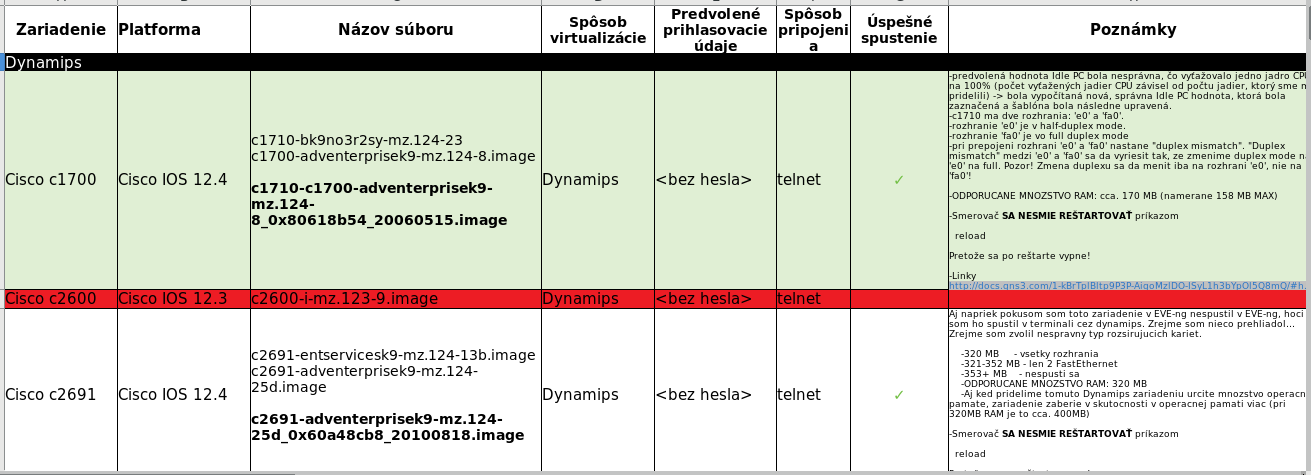
\includegraphics[width=1\textwidth,trim={0.1cm 0.3cm 0.1cm 0.2cm},clip]{sumarny_prehlad_testovanie_spustitelnosti}
    \caption{Tabuľkový dokument s výsledkami testovania spustiteľnosti}
    \label{obr:sumarny_prehlad_testovanie_spustitelnosti}
\end{figure}
}

\begin{longtabu} to \textwidth {| X[2.5,l,m] | X[5.0,l,m] |}
\caption{Popis stĺpcov v sumárnom prehľade zariadení}
\label{tab:sumarny_prehlad_stlpce} \\
\hline
    \multicolumn{1}{|c|}{\textbf{Stĺpec}} & \multicolumn{1}{|c|}{\textbf{Popis}} \\
\hline
    \textbf{Zariadenie} & \makecell[lc]{Názov alebo modelové označenie zariadenia.} \\
\hline
    \textbf{Platforma} & \makecell[lc]{Názov a verzia operačného systému zariadenia.} \\
\hline
    \textbf{Názov súboru} & \makecell[lc]{Pomenovanie zariadenia na serveri.} \\
\hline
    \textbf{Spôsob virtualizácie} & Hypervízor, pod ktorým zariadenie môže byť spustené. \\
\hline
    \textbf{\makecell[lc]{Predvolené prihlasovacie \\ údaje}} & Predvolené prihlasovacie meno a heslo, ak to zariadenie vyžaduje. \\
\hline
    \textbf{Spôsob pripojenia} & \makecell[lc]{Protokol, ktorý sa používa na vzdialenú konfiguráciu \\ zariadenia.} \\
\hline
    \textbf{Úspešné spustenie} & Informácia, či sa zariadenie v topológii spustilo. \\
\hline
    \textbf{Poznámky} & \makecell[lc]{Bližší popis správania sa daného zariadenia, popr. \\ problémy pri používaní zariadenia a ich možné riešenie. \\ Ďalej sa v ňom môžu nachádzať niektoré podporované \\ technológie a internetové odkazy ako zdroj pre informácie \\ uvádzané pre dané zariadenie. V časti v časti\\ \emph{Pridanie zariadenia} sú uvedené odkazy na pridanie\\ zariadenia do nástroja EVE-ng.} \\
\hline
\end{longtabu}

Ďalšie stĺpce slúžia pre prieskum spustiteľnosti zariadení v rôznych nástrojoch nasadených na rôznych platformách.

Pokiaľ sme zistili, že protokol vzdialeného prístupu sa odlišuje od predvoleného protokolu v šablóne na EVE-ng serveri, túto šablónu sme museli upraviť ručne. Avšak s postupným nárastom testovaných zariadení rástol aj počet úprav v šablónach pre jednotlivé zariadenia. Preto sme sa rozhodli vytvoriť skript (kap. \ref{chap:cd} bod \ref{item:uprava_sablon_skript}), ktorý by celý proces automatizoval. Tento skript na úpravu šablón upravuje jednotlivé atribúty konkrétnym zariadeniam. Výsledky testovania sa prejavili v skripte na úpravu šablón, v ktorom boli nastavené atribúty pre protokol na vzdialený prístup k zariadeniam, príp. vlastnosti rozširujúcich kariet zariadení.





\subsection{Testovanie systémových požiadaviek}
\label{chap:testovanie_zariadeni_benchmark}

Testovanie systémových požiadaviek zariadení bolo realizované na fyzickom EVE-ng serveri. Tento druh testovania bol dôležitý preto, aby sme mohli danému zariadeniu nastaviť dostatočné technické parametre, ktoré boli zmerané nástrojmi na meranie systémových prostriedkov. Tak zaistíme jeho plynulý chod a predídeme rôznym komplikáciám počas používania vo vyučovaní. Tieto parametre sú uložené v šablóne pre dané zariadenie.

Úprava šablón je realizovaná skriptom, po ktorého vykonaní sa príslušným zariadeniam zmenia konkrétne technické parametre v šablóne. Po úprave šablón sa zmeny prejavia okamžite a po pridaní zariadenia do topológie, kedy sa jeho parametre automaticky nastavia na správne hodnoty. Pre vybrané zariadenia boli merané tieto veličiny:

\begin{itemize}[noitemsep]
    \item Vyťaženie procesora
    \item Využitie operačnej pamäte
    \item Vyťaženie pevného disku
\end{itemize}

Vyťaženie procesora bolo merané z dôvodu jeho intenzívnej činnosti hlavne počas spúšťania zariadení, ale môže byť vyťažovaný aj po dokončení spúšťania. Na základe toho budeme vedieť určiť, koľko zariadení budeme môcť v topológii spustiť naraz, a koľko už spustených zariadení zvládne server spravovať celkovo. Pri meraní vyťaženia procesora bolo merané celkové vyťaženie aj vyťaženie jednotlivých jadier procesora.

Operačná pamäť je najviac využitá po dokončení spúšťania zariadenia. Kapacita operačnej pamäte ovplyvňuje celkový počet spustených zariadení na serveri. Meranie jej vyťaženia je pomerne jednoduché pre celý systém, ale pre tieto účely bolo potrebné s vysokou presnosťou vedieť, koľko operačnej pamäte využíva iba konkrétne zariadenie.

Na meranie využitia operačnej pamäte boli použité dva nástroje: \texttt{ps} a \texttt{ps\_mem}. Prvý z nich už bol na EVE-ng serveri prítomný, druhý bolo potrebné nainštalovať dodatočne. Na meranie boli použité dva nástroje, aby sa navzájom výsledky oboch nástrojov medzi sebou validovali.

Disk je najviac vyťažený predovšetkým pri spúšťaní zariadenia, ale môže byť vyťažený aj po dokončení spúšťania. Vyťaženie disku bolo do merania zahrnuté, aby sme vedeli odhadnúť, do akej miery je spúšťanie a beh zariadení ovplyvnené načítavaním zariadenia z pevného disku.

Z merania bola vynechaná frekvencia procesora a vyťaženie sieťového rozhrania. Frekvencia procesora bola vynechaná, lebo procesor podľa príkazu \texttt{watch lscpu | grep "MHz"} striedal iba dve frekvencie, 2000.000 MHz (minimálna frekvencia) a 2333.000 MHz (maximálna frekvencia), nezávisle na celkovom vyťažení procesora.

Vyťaženie sieťovej karty je zanedbateľné pri meraní výkonnosti jednotlivých zariadení, keďže sa sieť využíva iba na interakciu používateľa s klientskou aplikáciou, čo vytvára zanedbateľnú záťaž.

Na monitorovanie vybraných veličín sú určené rôzne nástroje a stratégie. Mohli sme napr. vytvoriť skript, ktorý by pomocou viacerých špecializovaných nástrojov meral vyťaženie jednotlivých prvkov systému, alebo použiť nástroj, ktorý je schopný monitorovať široké spektrum systémových zdrojov. Zvažovali sme tieto nástroje:

\begin{description}[noitemsep]
    \item [iotop] monitorovanie procesov podľa využitia disku
    \item [nmap] monitorovanie sieťovej prevádzky
    \item [nethogs] monitorovanie procesov podľa využitia sieťového rozhrania
    \item [dstat] monitorovanie rôznych systémových prostriedkov v CLI
    \item [sysstat] rovnako, ako nástroj \emph{dstat}
    \item [netdata] monitorovanie rôznych systémových prostriedkov cez webové rozhranie
\end{description}

Z uvedených nástrojov sme sa rozhodli použiť nástroj \emph{dstat}. Hlavným dôvodom, prečo sme sa rozhodli ďalej používať a upravovať tento nástroj a uprednostniť ho pred ostatnými nástrojmi, bolo predovšetkým ukladanie ziskaných údajov do CSV súboru. Dáta sa do CSV súboru zapisovali každú sekundu. Následne sme si vytvorili tabuľkový dokument, ktorý vyhodnocoval namerané dáta z CSV súboru. Vyhodnocovaním nameraných údajov sa budeme bližšie zaoberať v časti \ref{chap:testovanie_zariadeni_benchmark_vyhodnotenie}.

Nástroj \emph{dstat} však bolo potrebné upraviť tak, aby zisťoval využitie operačnej pamäte iba pre zariadenia v EVE-ng topológii, nie celého systému.

Pre tento účel sme vytvorili kópiu nástroja \emph{dstat} s názvom \emph{dstat\_custom}. V tejto kópii sme následne upravovali jeho zdrojový kód pre naše potreby. Nástroj \emph{dstat} bol vytvorený v programovacom jazyku Python.

Nástroj \emph{dstat\_custom} bol upravený tak, že meria využitie operačnej pamäte pre zariadenie v EVE-ng topológii nástrojmi \emph{ps} a \emph{ps\_mem}. Obidva príkazy merajú tú istú množinu procesov patriacu spustenému zariadeniu resp. spusteným zariadeniam topológii, aby sme mohli hodnoty oboch nástrojov medzi sebou porovnať. Hodnoty namerané obomi nástrojmi by mali byť približne rovnaké na to, aby sme mohli výsledky považovať za validné.

Vo výslednom CSV súbore vytvorenom nástrojom \emph{dstat\_custom} sa stĺpce \emph{used} a \emph{buffered} v časti \emph{memory usage} nahradia stĺpcami \emph{MemUsed-ps} a \emph{MemUsed-ps\_mem}.

Aby nástroj \emph{dstat\_custom} fungoval správne, musia byť nainštalované balíčky \emph{dstat}, \emph{ps\_mem} a \emph{sultan}. Význam prvých dvoch balíčkov už bol v tejto časti vysvetlený. Balíček \emph{sultan} slúžil na vykonávanie terminálových príkazov zvnútra Python programu.

Výsledky z merania systémových požiadaviek je takisto možné použiť v iných nástrojoch na sieťovú virtualizáciu. Pokiaľ existuje ekvivalentný typ zariadenia aj v inom nástroji, je odporúčané aplikovať namerané systémové parametre do jeho šablóny za predpokladu, že je pre zariadenie použitý rovnaký spôsob virtualizácie resp. hypervízor, napr. QEMU/KVM, Docker a pod.





\subsubsection{Metodika}

Najprv bol vytvorený zoznam vybraných zariadení, ktorých systémové požiadavky sme sa rozhodli testovať. Ten sa nachádza v kapitole \ref{chap:cd} v bode \ref{item:benchmarking_list} a na obr. \ref{obr:zoznam_zariadeni_test_sys_poziadaviek}. Zoznam zariadení bol vytvorený na základe kapitoly \ref{chap:analyza_vyucovania} - \nameref{chap:analyza_vyucovania}, keďže malo zmysel testovať iba tie zariadenia, ktoré by mohla katedra použiť vo vyučovaní.

\afterpage{
\begin{figure}
    \centering
    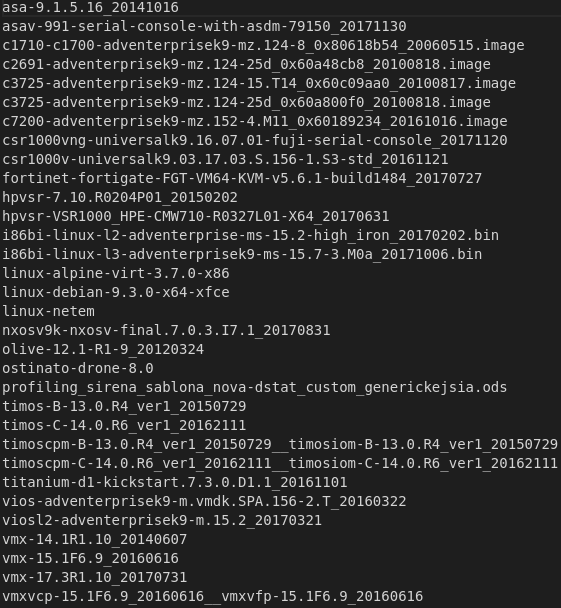
\includegraphics[width=0.7\textwidth,trim={0cm 8.1cm 0cm 0cm},clip]{zoznam_zariadeni_test_sys_poziadaviek}
    \caption{Textový dokument so zoznamom zariadení pre testovanie ich systémových požiadaviek}
    \label{obr:zoznam_zariadeni_test_sys_poziadaviek}
\end{figure}
}

Meranie systémových zdrojov zariadenia bolo vykonané nástrojom \emph{dstat\_custom}. Pred začiatkom každého merania bolo potrebné vykonať kroky, ktoré zvyšujú konzistenciu a presnosť výsledkov a reprezentujú najhoršie možné podmienky pre beh zariadenia. Všetky zariadenia sú uložené na rovnakom pevnom disku ako operačný systém.

Pred začatím merania výkonnosti každého zariadenia bolo v rámci úvodných krokov vypnuté používanie \emph{swap} partície a vyprazdnené vyrovnávacie časti operačnej pamäte (\emph{cache} a \emph{buffer}).

Na EVE-ng serveri bola počas celého merania vypnutá funkcia UKMS (Universal Kernel Samepage Merging). UKSM je mechanizmus, ktorý umožňuje šetriť využitie operačnej pamäte, keď je spustených viacero zariadení rovnakého typu. Ak je ale UKMS aktívne a spustíme viac ako 10 QEMU zariadení, ich výkon by mohol byť v dôsledku tohto mechanizmu znížený \cite{eve_ng_faq}.

\noindent
Meranie systémových požiadaviek zariadenia prebiehalo nasledovne:

\begin{enumerate}[noitemsep]
    \item Do EVE-ng predpripravenej prázdnej topológie pridáme zariadenie, ktoré chceme testovať.
    \item \label{nastavenie_sys_param} Nastavíme mu maximálne množstvo operačnej pamäte, s ktorým je zariadenie schopné úspešne sa spustiť. Ak je to možné, nastavíme počet procesorov na 1 CPU - tak bude záťaž na procesor minimalizovaná.
    \item Vykonáme vyššie uvedené úvodné kroky pred meraním.
    \item Nástrojom \emph{dstat\_custom} spustíme sledovanie systémových prostriedkov, ktorý bude ukladať namerané údaje do súboru.
    \item Spustíme zariadenie.
    \item Z nástroja zistíme čas spustenia zariadenia a zapíšeme si ho do osobitného súboru napr. \emph{boot\_time.txt}.
    \item Pripojíme sa na konzolu zariadenia. Počkáme, kým neuvidíme interaktívny príkazový riadok (CLI) alebo výzvu na prihlásenie.
    \item Ak je to nutné, po úspešnom spustení zariadenia sa naň prihlásime.
    \item Akonáhle uvidíme interaktívny príkazový riadok (CLI), do súboru \emph{boot\_time.txt} si uložíme čas, v ktorom zariadenie dokončilo svoje spúšťanie. 
    \item Zariadenie necháme 1-3 minúty stabilizovať.
    \item Ukončíme sledovanie systémových prostriedkov.
    \item Zastavíme zariadenie a odstránime ho z topológie.
\end{enumerate}

Pokiaľ sa vyskytli komplikácie so spúšťaním alebo behom zariadenia, vrátili sme sa na krok \ref{nastavenie_sys_param} a stanovili sme pre zariadenie iné systémové parametre. Systémové parametre zariadenia sme menili dovtedy, kým sa zariadenie nespustilo a odozva z klávesnice z jeho konzoly bola prijateľná. Podrobnejší popis rôznych konfigurácii systémových parametrov pre konkrétne zariadenia je k dispozícii v kapitole \ref{chap:cd} v bode \ref{item:sumarny_prehlad_zariadeni}

Po skončení merania vznikli dva nové súbory: súbor s nameranými údajmi a súbor s trvaním spúšťania zariadenia. Tieto súbory tvorili vstup pre tabuľkový súbor na vyhodnocovanie nameraných údajov pre zariadenie, ktorému sa venujeme v nasledujúcej časti.

Po ukončení merania všetkých zariadení môžeme znova zapnúť "swap" partíciu.





\subsubsection{Vyhodnotenie}
\label{chap:testovanie_zariadeni_benchmark_vyhodnotenie}

Po vytvorení súboru s nameranými údajmi a súboru s trvaním spúšťania zariadenia môžeme vložiť ich údaje do tabuľkového dokumentu. Na základe vstupných údajov sa automaticky prepočítajú výstupné hodnoty vo všetkých tabuľkách tohto dokumentu. Nižšie je opísaný priebeh vyhodnotenia nameraných údajov:

\begin{enumerate}[noitemsep]
    \item Do hárku \emph{SuroveUdaje} vložíme dáta namerané nástrojom \emph{dstat\_custom}.
    \item Do hárku \emph{VstupVystup} vložíme tieto údaje
    \begin{enumerate}[noitemsep]
        \item Do poľa \emph{Start} zadáme čas, kedy sme zariadenie spustili.
        \item Do poľa \emph{Stop} zadáme čas, kedy zariadenie dokončilo svoje spúšťanie a zobrazilo interaktívny príkazový riadok (CLI).
        \item Do poľa \emph{Množstvo voľnej RAM na serveri (MB)} zadáme množstvo voľnej operačnej pamäte na EVE-ng serveri v stave pokoja.
    \end{enumerate}
\end{enumerate}

Po zadaní spomenutých vstupných údajov tabuľkový dokument poskytne v hárku \emph{VstupVystup} odpovede na tieto otázky:

\begin{itemize}[noitemsep]
    \item Čas spúšťania - čas potrebný na dokončenie spúšťania zariadenia
    \item Odhadované množstvo operačnej pamäte pre jedno zariadenie / topológiu (MB)
    \item Odhadovaný počet zariadení, ktoré je možné naraz spustiť na základe celkového vyťaženia CPU
    \item Odhadovaný počet sputených zariadení na základe celkového vyťaženia CPU
    \item Odhadovaný počet sputených zariadení na základe voľnej RAM
\end{itemize}

Od všetkých vstupných údajov boli pred ďalším spracovaním odčítané namerané hodnoty z pokojového stavu EVE-ng servera.

Výsledky merania systémových požiadaviek zariadení reprezentujú najhorší možný scenár behu zariadenia.

Výsledky testovania vybraných zariadení sú prítomné v kapitole \ref{chap:cd} v časti \ref{item:all_benchmarks} \emph{eve-ng/profiling\_and\_benchmarking\_results}. Na obr. \ref{obr:testovanie_systemovych_poziadaviek_sablona} je ako príklad znázornený výstup tabuľkového súboru pre systémové požiadavky virtuálneho smerovača \emph{Cisco 7200}.

\begin{figure}
    \centering
    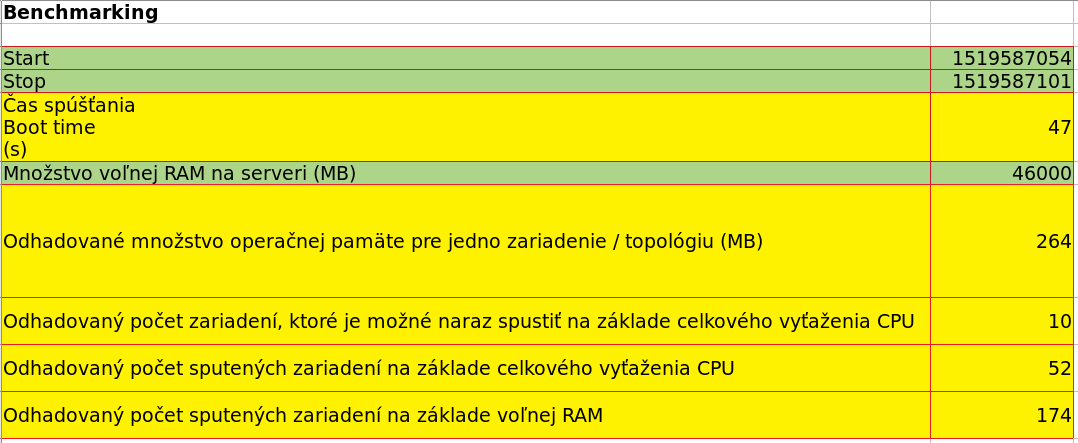
\includegraphics[width=1\textwidth,trim={0cm 0.1cm 0.1cm 0cm},clip]{testovanie_systemovych_poziadaviek_sablona}
    \caption{Tabuľkový dokument s nameranými systémovými požiadavkami}
    \label{obr:testovanie_systemovych_poziadaviek_sablona}
\end{figure}


Podľa tabuľkového dokumentu bolo pre každé zariadenie nastavené množstvo operačnej pamäte a počet CPU v skripte na úpravu šablón. Zariadenie vďaka tomu môžeme pridávať do topológie bez toho, aby sme museli premýšľať, či má nastavené dostatočné systémové parametre.

Celý proces merania systémových požiadaviek zariadení je bližšie vysvetlený v kapitole \ref{chap:cd} v bode \ref{item:benchmarking_popis}





\subsection{Testovanie technológii}
\label{chap:testovanie_technologii}

V tejto časti využijeme poznatky z kapitoly \ref{chap:analyza_vyucovania} - \nameref{chap:analyza_vyucovania} a použijeme ich na testovanie, či vybrané zariadenia podporujú témy vyučované na katedre. Testované boli iba podporované technológie Cisco zariadení, keďže tie sa používajú vo vyučovaní najviac.

Cieľom testovania technológii je zistiť, do akej je možné použiť virtuálne zariadenia pri vyučovaní takých tém, na ktoré boli doposiaľ použité fyzické zariadenia alebo virtualizačné riešenia s užším rozsahom podporovaných technológii. Jednalo sa najmä o podporu prepínacích technológii na predmetoch \emph{Pokročilé prepínanie v informačno-komunikačných sieťach} (CCNP Switching) a \emph{Počítačové siete 1} (CCNA 2 + prepínacie technológie). Prioritné boli testované témy vyučované na CCNP kurze, keďže prepínacie technológie v CCNP kurze zahŕňajú aj tie zo CCNA.





\subsubsection{Metodika}

Na testovanie podporovaných technológii vybraných zariadení bol vytvorený skript, ktorý je dostupný v kapitole \ref{chap:cd} v bode \ref{item:cisco_feature_testing_skript} a znázornený na obr. \ref{obr:skript_testovanie_podporovanych_technologii_cisco}. Skript sa skladal z viacerých skupín konfiguračných príkazov, pričom každá skupina mala za úlohu testovať podporu konkrétnej technológie na zariadení. Časti tohto skriptu boli postupne zadávané do konfigurácie zariadenia.

Nižšie je uvedený zoznam testovaných zariadení pre tento účel:

\begin{itemize}[noitemsep]
    \item Cisco IOL prepínač
    \item Cisco vIOS prepínač
    \item Cisco 3725 s EtherSwitch modulom
    \item Cisco 7200
    \item Cisco IOL smerovač
    \item Cisco vIOS smerovač
    \item Cisco CSR
    \item Cisco CSR-ng
\end{itemize}

\begin{figure}
    \centering
    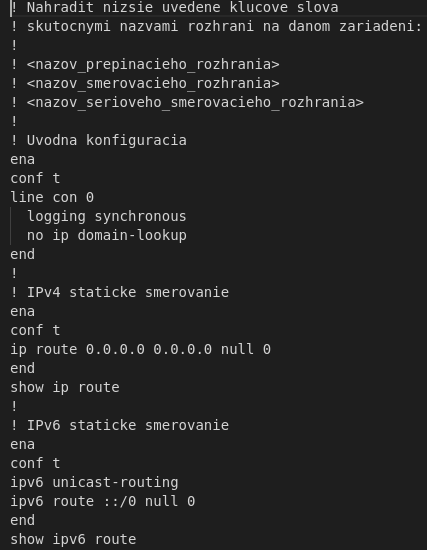
\includegraphics[width=0.35\textwidth,trim={0cm 0cm 5cm 4.65cm},clip]{skript_testovanie_podporovanych_technologii_cisco}
    \caption{Skript na testovanie podporovaných technológií pre Cisco zariadenia}
    \label{obr:skript_testovanie_podporovanych_technologii_cisco}
\end{figure}


\subsubsection{Vyhodnotenie}
\label{chap:testovanie_technologii_vyhodnotenie}

Po vykonaní konfiguračných príkazov zo skriptu bolo potrebné vyhodnotiť, či a do akej miery je testovaná technológia na danom zariadení podporovaná. Technológia bola označená ako podporovaná vtedy, ak príkaz nevypísal žiadne chybové hlásenie. V opačnom prípade sa testovali alternatívne konfigurácie. Ak sa ani žiadna z alternatívnych konfigurácii nevykonala úspešne, technológia bola vyhodnotená ako nepodporovaná. Výsledky testovania technológii sú dostupné v kapitole \ref{chap:cd} v bode \ref{item:zoznam_technologii_s_podporou_zariadeni} a ukážka tohto tabuľkového dokumentu je znázornená na obr. \ref{obr:zoznam_technologii_s_podporou_zariadeni}. V stĺpci \emph{Technológia} sa nachádza názov vyučovanej témy. Stĺpec \emph{Predmety} obsahuje skratku predmetu, na ktorej je táto téma vyučovaná. Podporované vyučované témy jednotlivých testovaných zariadení sú farebne odlíšené, popr. doplnené krátkym komentárom.

%\afterpage{
\begin{figure}
    \centering
    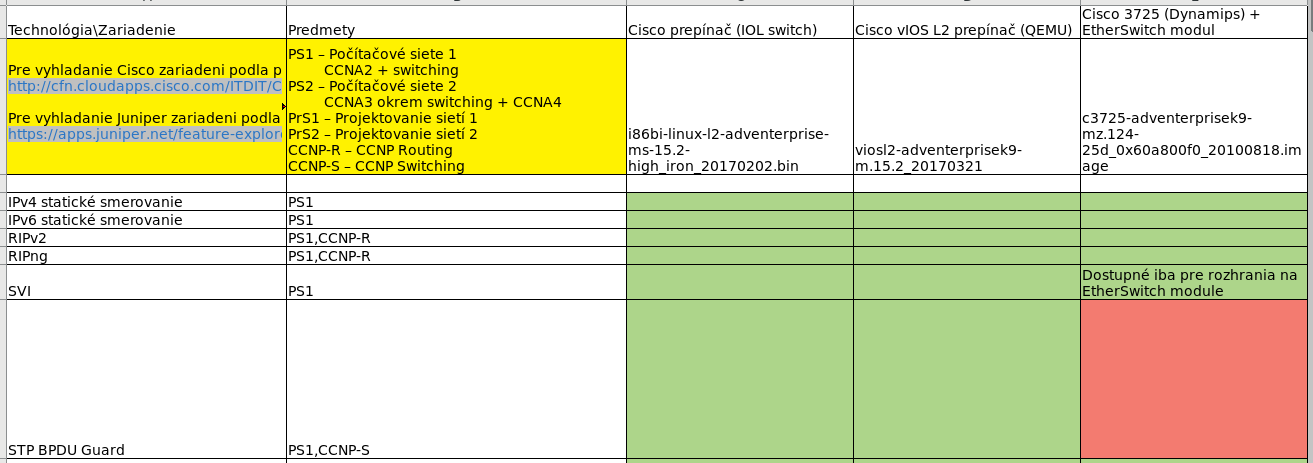
\includegraphics[width=1\textwidth,trim={0.2cm 0.15cm 0.15cm 0.15cm},clip]{zoznam_technologii_s_podporou_zariadeni}
    \caption{Tabuľkový súbor s podporovanými technológiami pre jednotlivé zariadenia}
    \label{obr:zoznam_technologii_s_podporou_zariadeni}
\end{figure}
%}

Zo spomenutého súboru vyplýva, že prepínacie technológie sú dostupné iba na zariadeniach \emph{Cisco IOL prepínač} a \emph{Cisco vIOS prepínač}. EtherSwitch modul na prepínači Cisco 3725 síce podporoval niektoré prepínacie technológie, ale bolo ich výrazne menej. Prepínacími technológiami sa zaoberajú hlavne predmety Počítačové siete 1 a Pokročilé prepínanie v informačno-komunikačných sieťach.

Špeciálne postavenie má \emph{Cisco IOL smerovač}, ktorý ako jediný v EVE-ng obsahuje sériové rozhrania, preto aj ako jediný v EVE-ng podporuje Point-to-point technológie. Tento druh smerovača je dôležité pre predmety Počítačové siete 1/2 a Pokročilé prepínanie/smerovanie v informačno-komunikačných sieťach. Ďalšou zvláštnosťou je, že v EVE-ng nie je možné odchytávať prevádzku pre sériové rozhranie. Zaujímavosťou je, že zo všetkých testovaných smerovačov mal najnižšie spotrebu operačnej pamäte, cca 250 MB. V nástroji EVE-ng je prítomný Cisco IOL smerovač z roku 2017 s operačným systémom \emph{IOS 15.7-3.M0a}.

Ukázalo sa, že smerovače \emph{Cisco 3725}, \emph{Cisco 7200}, \emph{Cisco IOL smerovač} a \emph{Cisco vIOS smerovač} majú veľmi podobnú množinu funkcií, až na malé odchýlky. Cisco 3725 s EtherSwitch modulom ako jediný spomedzi nich podporuje SVI, PortFast, 802.1Q Trunk, VTPv1/v2, STP, HSRP a HSRPv2 (obe pre IPV4), VRRPv2, SPAN a IGMP Snooping. avšak nepodporuje GLBP IPv6 ani EIGRP IPv6. Prepínacie technológie sú dostupné iba pre rozhrania v EtherSwitch module. Spomínané 4 smerovače je možné použiť v topológiách pre uzly, ktoré nevyžadujú sériové prepojenia v rámci ľubovoľného predmetu.

Smerovače \emph{Cisco CSR} a \emph{Cisco CSR-ng} sú vhodné na pokročilejšie sieťové technológie, ako napr. VPLS, vyučovaných na predmetoch Projektovanie sietí 1/2. Zvláštnosťou je chýbajúca podpora GLBP pre IPv6 na \emph{Cisco CSR}. Zaujímavou je podpora niektorých prepínacích technológii pre Cisco CSR-ng a v menšej miere pre Cisco CSR, hoci je ich ešte menej, ako pri smerovači Cisco 3725. Nevýhodou oboch smerovačov, v porovnaní s ostatnými šiestimi, sú ich vyššia spotreba operačnej pamäte, cca 4,5 GB.

Výsledky tohto prieskumu boli použité v poslednej fáze projektu - \nameref{chap:nasadenie_do_vyucovania}, ktorej sa venujeme v kapitole \ref{chap:nasadenie_do_vyucovania}. Vyhodnotenie slúži iba na odhad, ktoré zariadenia majú najväčšiu pravdepodobnosť využitia na danom predmete. V prípade, že má predmet v zozname viacero zariadení, treba sa na základe ďalších kritérií rozhodnúť, ktoré z nich budú použité v topológii. Môžeme napr. brať do úvahy iné vyučované témy v topológii, systémové požiadavky zariadenia, iné technické obmedzenia zariadenia a pod. V každom prípade je potrebné pred vytvorením akejkoľvek topológie použiť zoznam podporovaných funkcií pre zariadenia v kapitole \ref{chap:cd} v bode \ref{item:zoznam_technologii_s_podporou_zariadeni} 
\chapter{Nasadenie do vyučovania}
\label{chap:nasadenie_do_vyucovania}

Aby bola preverená celková kvalita a využiteľnosť virtuálneho laboratória, bol nástroj EVE-ng nasadený na vypracovávanie rôznych topológii z vybraných predmetov, ktoré sú opísané v nasledujúcich častiach tejto kapitoly. Zároveň budú popísané aj problémy, ktoré proces nasadzovania sprevádzali. Predmety sú uvedené v poradí podľa toho, v akom čase bol nástroj EVE-ng na nich používaný. Návod na vytvorenie vlastnej topológie je uvedený v kapitole \ref{chap:pouzivanie_eve_ng}.





\section{Projektovanie sietí 2}

V rámci predmetu Projektovanie sietí 2 bol nástroj EVE-ng nasadený do vyučovania na vypracovávanie topológii s pokročilejšími sieťovými technológiami. Topológie boli spustené na virtuálnom EVE-ng serveri.

V EVE-ng boli úspešne dokončené semestrálne práce zamerané na pokročilé technológie v témach z oblastí \emph{VPLS} a \emph{Seamless MPLS}. Téma \emph{EVPN} bola vypracovávaná v nástroji \emph{ViRo2}.

Topológie semestrálnych prác sa skladali z týchto zariadení:

\begin{itemize}[noitemsep]
    \item Cisco IOL smerovač - VPLS, Seamless MPLS
    \item Cisco CSR - VPLS
    \item Juniper Olive - Seamless MPLS
    \item Juniper vMX 15 - VPLS
    \item Nokia VSR - EVPN
\end{itemize}

Vypracovávanie semestrálnych prác sa však nezaobišlo bez komplkácii. Neustále bola zapracovávaná spätná väzba študentov pracujúcich v skupinách ohľadom používania nástroja EVE-ng a podporovaných technológii zariadení. Zistilo sa napríklad, že virtuálna inštalácia EVE-ng neposkytuje dostatočný výkon, ktorý bol potrebný na vypracovanie všetkých semestrálnych prác. Preto bol vytvorený fyzický EVE-ng server, ktorý bol nasadený na nasledujúcom predmete, Počítačové siete 2.





\section{Počítačové siete 2}

V rámci predmetu Počítačové siete 2 bol nástroj EVE-ng nasadený do vyučovania na vypracovávanie topológii s \emph{point-to-point} technológiami. Topológie boli spustené na fyzickom EVE-ng serveri. V prípade zlyhania EVE-ng boli pripravené aj záložné topológie v nástroji Dynamips/Dynagen.

Najprv bola vytvorená základná topológia, znázornená na obrázku \ref{obr:eve_ng_ppp_zakladna_topo_v2}. Tá pozostávala zo štyroch Cisco IOL smerovačov a dvoch koncových zariadení s operačným systémom Alpine Linux. Cisco IOL smerovač bol vybraný, pretože ako jediný podporoval sériové rozhrania a \emph{point-to-point} technológie. Koncové zariadenie Alpine Linux bolo vybrané pre svoju nenáročnosť na systémové zdroje.

Celkovo bolo vytvorených 8 zhodných topológii, ktoré medzi sebou zdieľali jeden učiteľský smerovač. V topológii sa celkovo nachádzalo 33 Cisco IOL smerovačov a 16 koncových staníc. Celková topológia sa nachádza na obrázku \ref{obr:eve_ng_ppp_celkova_topo_v2}.

\begin{figure}
    \centering
    \includegraphics[width=0.6\textwidth,trim={2cm 0cm 2cm 2.5cm},clip]{eve_ng_ppp_zakladna_topo_v2}
    \caption{Základná PPP topológia}
    \label{obr:eve_ng_ppp_zakladna_topo_v2}

    \vspace{3cm}

    \centering
    \includegraphics[width=1.0\textwidth,trim={4cm 10cm 0.5cm 4cm},clip]{eve_ng_ppp_celkova_topo_v2}
    \caption{Celková PPP topológia}
    \label{obr:eve_ng_ppp_celkova_topo_v2}
\end{figure}

IOL smerovače fungovali, až na príkaz \texttt{clock rate} na sériových rozhraniach, bez chyby. Ukázalo sa, že nastavenie DCE/DTE závisí od párnosti čísla skupiny. Párne číslo skupiny sériových rozhraní bude vždy DTE, nepárne vždy DCE, ako je zrejmé z obrázku \ref{obr:eve_ng_dce_dte_2E8S}. Rozdelenie sériových rozhraní na DCE/DTE nezávislé od počtu ethernetových alebo sériových skupín, čo potvrdzuje obrázok \ref{obr:eve_ng_dce_dte_1E8S}. Nastavenie DTE/DCE módu pre sériové rozhrania je v EVE-ng pri Cisco IOL smerovačoch pevne dané a nedá sa zmeniť, na čo treba myslieť pri návrhu topológie. Pre porovnanie, v nástroji Dynamips/Dynagen sa dá DCE/DTE mód na jednotlivých sériových rozhraniach ľubovoľne meniť.

\begin{figure}
    \centering
    \includegraphics[width=0.7\textwidth]{eve_ng_dce_dte_2E8S}
    \caption{Typy sériových rozhraní na IOL smerovači - 2 ethernetové + 8 sériových skupín}
    \label{obr:eve_ng_dce_dte_2E8S}

    \vspace{1cm}

    \centering
    \includegraphics[width=0.7\textwidth]{eve_ng_dce_dte_1E8S}
    \caption{Typy sériových rozhraní na IOL smerovači - 1 ethernetová + 8 sériových skupín}
    \label{obr:eve_ng_dce_dte_1E8S}
\end{figure}

V jednej študentskej skupine sa vyskytol problém s jednosmernou PAP autentifikáciou študentského smerovača voči učiteľskému (R\_Ucitel(s4/1)-5R2(s2/1)). Príkaz \\\texttt{debug ppp authentication} hlásil chybu pri autentifikácii. Riešenie spočívalo v odstránení používateľa, vypnutí \emph{ppp} konfigurácie a vypnutí rozhraní. Všetky tieto kroky boli vykonané aj na učiteľskom, aj na študentskom smerovači. Následne sa konektivita obnovila a spojenie pomocou PAP autentifikácie sa úspešne nadviazalo.

Je možné, že problémy vznikli aj kvôli tomu, že medzi študentským a učiteľským smerovačom boli na oboch stranách sériové rozhrania párnej skupiny t.j. obidva konce linky boli typu DTE. Niektoré skupiny študentov boli tiež pripojené k učiteľskému smerovaču sériovým rozhraním z párnej skupiny, ale takéto problémy nezaznamenali. Podobne tomu bolo aj pri prepojení Cisco IOL smerovačov rozhraniami DCE.

Z toho vyplýva, že Cisco IOL smerovače v EVE-ng majú pri prepojení dvoch smerovačov sériovou linkou s rovnakým módom nedefinované správanie. Tomu sa dá predísť vhodným návrhom topológie. Ten spočíva v tom, že sériové rozhrania medzi smerovačmi kombinujeme tak, aby bolo prepojené vždy sériové rozhranie párnej skupiny na jednom smerovači so sériovým rozhraním nepárnej skupiny na inom smerovači t.j. \emph{Serial2/x} (DCE) na prvom smerovači sa musí pripojiť napr. k \emph{Serial3/x} na druhom. V takom prípade DCE koniec po nastavení \texttt{clock rate} v príkaze \texttt{show controllers} zobrazí nastavený atribút \emph{received clockrate}, DTE koniec naproti tomu zobrazí hodnotu \emph{n/a}. Napriek tomu konektivita po správnom nastavení IP adries a zapnutí rozhraní bola aktívna.

Komplikácie s DCE/DTE a PPP autentifikáciou boli prítomné v prvom návrhu topológie, ktorý je znázornený na obrázku \ref{obr:eve_ng_ppp_zakladna_topo_v1}.

Pri testovaní DCE/DTE rozhraní sme narazili na obmedzenie nástroja EVE-ng. Community verzia je totiž dovoľuje v jednej topológii mať spustených najviac 63 zariadení. Po spustení 64. sa na niekoľko sekúnd spustí, ale nakoniec sa automaticky vypne. Community verzia vie spustiť aj viac ako 64 zariadení v jednej topológii, ale vo výsledku sa spustia len niektoré, na prvý pohľad náhodne vybrané zariadenia. Avšak tie zariadenia, ktoré sa spustia, pracujú štandardným spôsobom. Uvedený problém sa nám nepodarilo vyriešiť ani rozšírením rozsahu portových čísel pre zariadenia v topológii.
  
Zmerané boli aj systémové požiadavky celkovej topológie na fyzickom EVE-ng serveri. Po vyhodnotení výsledkov merania sme zistili, že celá topológia, 33 Cisco IOL smerovačov a 16 koncových zariadení Alpine Linux, sa spúšťala približne 2 minúty, spotrebovala 13GB operačnej pamäte a procesor vyťažovala na 21\%. Celkovo by sme podľa celkového vyťaženia CPU mohli spustiť 4 takéto topológie, avšak množstvo operačnej pamäte by dovoľovalo spustiť iba 3. Tabuľkový dokument s výsledkami merania systémových požiadaviek topológie je prítomný v kapitole \ref{chap:cd} v bode \ref{item:nasadenie_ps2_benchmark}

Spomenutý súbor ukazuje veľké rozdiely v meraniach využitia operačnej pamäte medzi nástrojmi \emph{ps} a \emph{ps\_mem} v hárku \emph{VstupVystup}, hoci sa merala rovnaká množina procesov. Po manuálnom overení sa ukázalo, že prvý menovaný nástroj vykazoval presnejšie výsledky, preto boli pri odhadoch použité ním namerané hodnoty.

\begin{figure}
    \centering
    \includegraphics[width=0.5\textwidth,trim={12cm 2cm 23.7cm 7cm},clip]{eve_ng_ppp_zakladna_topo_v1}
    \caption{Základná PPP topológia - prvotný návrh}
    \label{obr:eve_ng_ppp_zakladna_topo_v1}
\end{figure}





\section{Projektovanie sietí 1}

V rámci predmetu Projektovanie sietí 1 bol nástroj EVE-ng nasadený do vyučovania na vypracovanie topológií na tému \emph{MPLS}. V prípade zlyhania EVE-ng boli pripravené aj záložné topológie v nástroji Dynamips/Dynagen.

Najprv bola stanovená základná topológia (obr. \ref{obr:mpls_zakladna_topo}). Od nej sa odvíjali ostatné topológie. Celkovo bolo použitých týchto 6 typov zariadení:

\begin{itemize}[noitemsep]
    \item Cisco IOL prepínač
    \item Cisco IOL smerovač
    \item Cisco 3725 smerovač (Dynamips) s EtherSwitch modulom
    \item Cisco 7200 smerovač (Dynamips)
    \item Cisco vIOS smerovač (QEMU)
    \item Cisco vIOS prepínač (QEMU)
\end{itemize}

Topológie pozostávali z 10 Cisco smerovačov resp. Cisco MLS. Z každého typu boli spustené 2 topológie t.j. 20 zariadení, okrem Cisco vIOS a vIOS L2 prepínača, z ktorých bola vytvorená iba jedna pre každý typ. 

Rôzne zariadenia sa použili preto, aby boli otestované funkcie ich jednotlivých typov. Pokiaľ by sa ukázalo, že viaceré zariadenia podporujú nutné technológie, môžeme v budúcnosti použiť iba tie, ktoré vyžadujú najmenšie systémové prostriedky. Tak sa dá maximalizovať množstvo spustených zariadení.


\begin{figure}
    \centering
    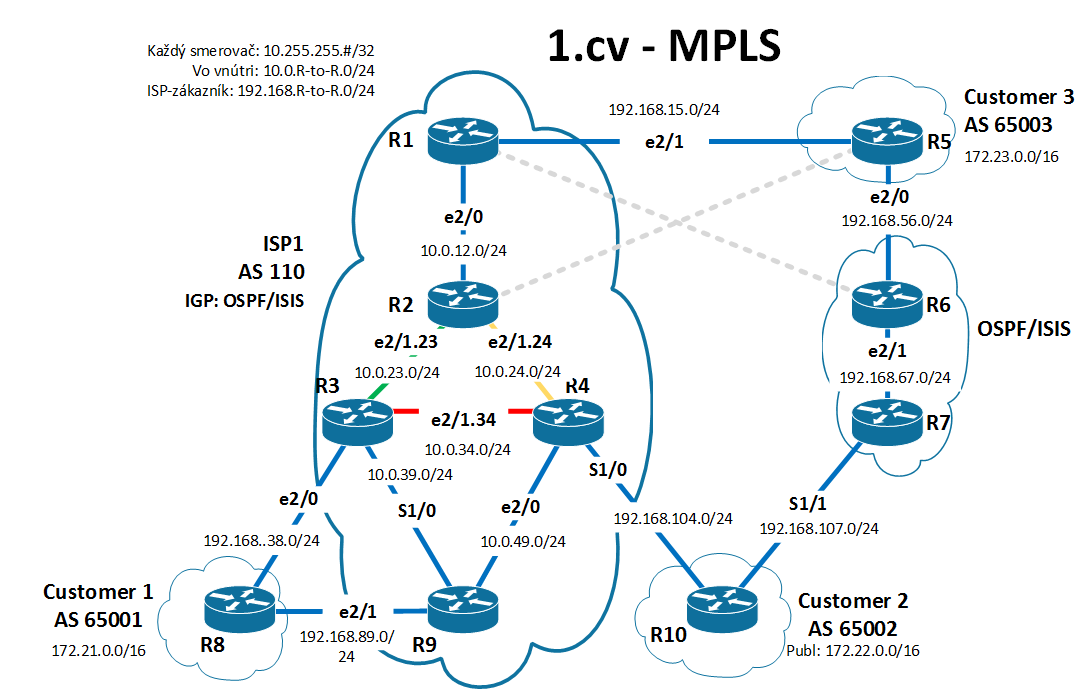
\includegraphics[width=1\textwidth,trim={0cm 0cm 0cm 0cm},clip]{mpls_zakladna_topo}
    \caption{Základná MPLS topológia}
    \label{obr:mpls_zakladna_topo}
    \cite{mpls_zakladna_topo}
\end{figure}

Študenti boli rozdelení do 10 skupín po dvoch študentoch. Z toho vyplýva, že bolo potrebné spustiť najmenej 10 topológii t.j. celkovo 100 zariadení.

Avšak EVE-ng vo verzii \emph{Community} dokáže v jednej topológii stabilne spustiť najviac 63 zariadení. Preto boli vytvorené dva používateľské účty s rolou \emph{editor}. V oboch účtoch bolo vytvorených 6 topológii, pre každý typ zariadenia jedna. Pre spomenuté používateľské účty bol vybraný taký \emph{POD} identifikátor, aby sa portový rozsah začínal číslom 1, aby to zodpovedalo názvu smerovača prvého smerovača, R1. Zvolené identifikátory boli \emph{9} pre prvého a \emph{14} pre druhého používateľa.

Topológie boli vytvárané tak, aby bol zachovaný počet zariadení a ich prepojenia medzi nimi. Avšak názvy rozhraní rôznych typov zariadení neboli vždy rovnakého typu alebo neboli rovnako očíslované. Preto boli rozhrania pre jednotlivé typy zariadení vybrané tak, aby logicky podľa jednoduchého pravidla zodpovedali tým v pôvodnej topológii. Napr. Cisco IOL zariadenia mali 3 skupiny \emph{Ethernet} rozhraní namiesto dvoch, aby sa názvy rozhraní zhodovali s pôvodným návrhom MPLS topológie (e2/x).

Súčasťou topológie je aj \emph{bridge} zariadenie, ktorého úlohou je iba vytvoriť \emph{broadcast} doménu medzi smerovačmi R2, R3 a R4 a preposielať v rámci nej rámce. Výhodou takéhoto zariadenia sú minimálne požiadavky na systémové prostriedky, keďže po jeho vytvorení sa vytvorený iba \emph{bridge} rozhranie na serveri.

Každému študentovi bol vytvorený používateľský účet s rolou \emph{user}. Tento účet mal slúžiť na prehliadanie topológie priradenej danej skupine. V momente, keď sa študenti začali prihlasovať do webového rozhrania EVE-ng a začali otvárať potrebné súbory s topológiami, server v dôsledku tejto záťaže vykazoval maximálne vyťaženie a stal sa nestabilným. Nestabilita bola vyriešená ukončovaním výpočtovo náročných procesov pomocou vzdialeného prístupu cez SSH. Ukázalo sa, že otváranie topológie je v nástroji EVE-ng výpočtovo náročná činnosť Tomuto problému sa dá predísť tak, že topológie budú jednotliví používatelia otvárať postupne, jeden po druhom. Pri sledovaní záťaže počas otvárania topológie server vykazoval vyššiu záťaž, ktorá sa po dokončení načítavania ustálila.

Nakoniec si všetci študenti otvorili príslušné súbory s topológiou, aby videli, ktoré rozhrania je potrebné jednotlivým zariadeniam konfigurovať. Súbory s topológiou slúžili ako doplnok ku pôvodnému návrhu topológie, ktorý obsahoval dodatočné informácie, ako sú adresácia a čísla autonómnych systémov pre BGP.

Žiaľ, študenti nevypracovali topológiu na tému MPLS v nástroji EVE-ng, pretože dokončovali úlohy z predchádzajúcich cvičení.




\section{Vyhodnotenie}

Z predmetov Počítačové siete 1, Pokročilé prepínanie v informačno-komunikačných sieťach a Pokročilé smerovanie v informačno-komunikačných sieťach neboli vypracované žiadne topológie.

Na predmetoch, kde nástroj EVE-ng nasadený bol, sa ukázalo, že ho je možné používať vo vyučovaní.

Pri nasadení na predmet Projektovanie sietí 2, kde bola použitá virtuálna inštalácia EVE-ng, bol naopak nástroj nestabilný, zariadenia často zamŕzali a pri zadávaní príkazov do konzoly bola prítomná vyššia odozva z klávesnice. Mohlo to byť spôsobené mnohými faktormi, či už samotnou virtuálnou platformou VMware, alebo nesprávne nastavenými systémovými parametrami pre jednotlivé zariadenia v topológii.

Študenti počas vypracovávaní topológie na predmete Počítačové siete 2 nezaznamenali žiadny rozdiel oproti nástroju Dynamips/Dynagen, keďže sa na zariadenia prihlasovali rovnako, pomocou nástroja \emph{PuTTY} IP adresou a portom, pričom zariadenia poskytovali, až na malé výnimky rovnaké funkcie, ako v nástroji Dynamips/Dynagen. Nástroj EVE-ng na fyzickom serveri bol počas celej doby vypracovávania stabilný. Zariadenia boli počas celého vyučovania spustené a samovoľne sa nevypínali.

Napriek mnohým nedostatkom nástroja EVE-ng, je minimálne pre učiteľov výhodou, že môžu vytvárať topológie z grafického rozhrania, namiesto z príkazového riadku. Nevýhodami sú nemožnosť stabilne spúšťať viac ako 63 zariadení v jednej topológii. Jednotliví používatelia a študenti si svoje topológie nemôžu spravovať nezávisle na sebe, keďže toto je možné iba v Learning Centre verzii nástroja, ktorá súbory jednotlivých používateľov od seba oddeľuje.

Čo sa týka odhadov systémových požiadaviek topológii, tie môžeme odhadnúť súčtom systémových požiadaviek jednotlivých zariadení, ktoré sa v topológii budú nachádzať. Systémové požiadavky vybraných zariadení sú k dispozícii na CD v kapitole \ref{chap:cd} v bode \ref{item:all_benchmarks}
\chapter{Záver}

Cieľom práce bolo nasadenie virtuálneho sieťového laboratória do vyučovacieho procesu katedry. Najprv bolo potrebné preskúmať existujúce riešenia pre virtuálne sieťové laboratóriá a porovnať ich na základe zvolených kritérií. Z porovnania vyplynulo, že existujú viaceré virtuálne laboratória, ktorými sa má zmysel ďalej zaoberať: GNS3 a EVE-ng. Nakoniec však bol zvolený druhý menovaný nástroj. Následne bol tento nástroj nainštalovaný na virtuálnu platformu VMware a fyzický server.

Po nasadení nástroja do infraštruktúry katedry boli analyzované vyučované témy vybraných predmetov na Katedre informačných sietí. Táto analýza pomohla pri získavaní virtuálnych zariadení do nástroja EVE-ng. Získané zariadenia boli v nástroji EVE-ng testované na ich spustiteľnosť, systémové požiadavky a podporu vyučovaných tém. Pre analyzované predmety boli vybrané zariadenia, ktoré boli počas nasadenia do vyučovania použité pri vytváraní topológii. Zariadenia boli pre predmety vyberané tak, aby pokryli čo najväčšiu časť vyučovaných tém. Študenti na cvičeniach pod vedením vyučujúceho používali tento nástroj, aby sa overila jeho použiteľnosť v reálnom vyučovacom procese.

Celý proces bol dôsledne a prehľadne dokumentovaný. Dokumentácia podrobne opisuje celý proces práce od inštalácie nástroja EVE-ng a jeho následnej úpravy až po získavanie a testovanie virtuálnych zariadení a nasadenie nástroja do vyučovania. Dokumentácia je prítomná na priloženom CD, ktorého adresárovú štruktúru je možné vidieť v kapitole \ref{chap:cd}.

Na výsledkoch tejto práce sa dá v budúcnosti pokračovať v mnohých smeroch. Práca môže slúžiť ako východiskový bod pri skúmaní ďalších virtuálnych sieťových laboratórií s použitím metodík popísaných v rôznych častiach tejto práce. To by mohlo viesť k vytvoreniu ideálneho riešenia pre virtuálne sieťové laboratórium, ktoré by v sebe kombinovalo výhody nástrojov ViRo2, GNS3 a EVE-ng, pričom jadro by tvoril práve nástroj GNS3. Ideálne sieťové laboratórium by obsahovalo rezervácie topológii z nástroja ViRo2, grafické používateľské rozhranie, jednoduchú škálovateľnosť naprieč viacerými servermi, dodatočnú podporu Docker popr. LXC/LXD kontajnerov a izoláciu používateľov spolu ich súbormi a adresármi. Vo svojej práci som sa snažil splniť aspoň niektoré zo spomenutého stručného zoznamu požiadaviek.

Ďalším krokom v pokračovaní projektu by mohlo byť nasadenie nástroja EVE-ng resp. GNS3 do LXC kontajnera pre lepšiu škálovateľnosť. Takisto by bolo zaujímavé preskúmať využitie katedrového OpenStack riešenia ako virtuálne sieťové laboratórium.

V každom prípade nasadenie konkrétneho nástroja do vyučovacieho procesu katedry posunulo vyučovanie na nej na vyššiu úroveň, čo dokazuje, že virtuálne sieťové laboratórium tvorí dôležitú súčasť pri vyučovaní sieťových technológii.
\chapter{Prílohy}
\label{chap:prilohy}





\section{CD}
\label{chap:cd}


\begin{enumerate}[noitemsep,label*=\thesection.\arabic*.]
    \item diplomova\_praca
    
    \begin{enumerate}[noitemsep,label*=\arabic*.]
        \item praca
        
        \begin{enumerate}[noitemsep,label*=\arabic*.]
            \item kapitoly
            \item obrazky
            \item uvodne\_strany
            \item praca.pdf
        \end{enumerate}
        
        \item zadanie\_diplomovej\_prace.pdf
    \end{enumerate}
    
    \item \label{item:prilohy_cd_eve_ng_adresar} eve\_ng
    
    \begin{enumerate}[noitemsep,label*=\arabic*.]
        \item profiling\_and\_benchmarking\_results
        
        \begin{enumerate}[noitemsep,label*=\arabic*.]
            \item 0\_pokojovy\_stav
            \item \label{item:all_benchmarks} adresáre s meraniami systémových požiadaviek pre každé zariadenie
        \end{enumerate}
        
        \item \label{item:skripty} skripty
        
        \begin{enumerate}[noitemsep,label*=\arabic*.]
            \item \label{item:uprava_sablon_skript} 10\_1\_update\_eve\_ng\_templates.sh
            \item \label{item:backup_script} 12\_1\_backup\_gns3\_and\_eveng\_data\_to\_backup\_server.sh
            \item \label{item:gns3_import_skript} import\_eveng\_qemu\_devices\_to\_gns3.sh
        \end{enumerate}
        
        \item \label{item:vnc1} 01\_0\_vytvorenie\_vzdialenej\_pracovnej\_plochy\_nomachine.txt
        \item \label{item:vnc2} 01\_1\_vytvorenie\_vzdialenej\_pracovnej\_plochy\_vnc.txt
        \item \label{item:vnc3} 01\_2\_vytvorenie\_vzdialenej\_pracovnej\_plochy\_\_x2go\_BROKEN\_IN\_\\STRETCH
        \item \label{item:vmware_extra_instalacia} 02\_instalacia\_vmware\_player\_debian.txt
        \item 03\_hardverova\_konfiguracia\_EVE\_vo\_VMware\_Player.txt
        \item \label{item:instalacia_ubuntu_a_eve_ng} 04\_0\_instalacia\_eve\_ng.txt
        \item 04\_1\_instalacia\_eve\_ng\_do\_lxc\_kontajnera.txt
        \item \label{item:instalacia_A_konfiguracia_eve_ng} 05\_0\_prvotna\_konfiguracia\_EVE\_ng.txt
        \item \label{item:adresarova_struktura} 05\_1\_adresarova\_struktura\_uzitocne\_eve-ng\_subory.txt
        \item \label{item:zabezpecenie} 06\_zabezpecenie\_servera.txt
        \item 07\_0\_podporovane\_zariadenia\_v\_UNetLab\_EVE-ng.txt
        \item \label{item:pridavanie_konverzia_zariadeni} 07\_1\_pridavanie\_a\_konverzia\_zariadeni.txt
        \item 07\_2\_vypocet\_idle\_pc\_hodnot\_pre\_dynamips\_zariadenia.txt
        \item 07\_3\_pridanie\_cisco\_c2691\_do\_eve\_ng-CIASTOCNY\_USPECH.txt
        \item \label{item:pridavanie_juniper_vmx} 07\_4\_pridavanie\_zariadeni\_do\_eve\_ng\_juniper\_vmx\_17.3.txt
        \item 07\_5\_pridavanie\_zariadeni\_do\_eve\_ng\_cisco\_prime\_infra.txt
        \item 07\_6\_pridavanie\_zariadeni\_do\_eve\_ng\_vyos.txt
        \item 07\_7\_pridavanie\_zariadeni\_do\_eve\_ng\_pfsense.txt
        \item \label{item:pridavanie_cisco_asav} 07\_8\_pridavanie\_zariadeni\_do\_eve\_ng\_cisco\_asav.txt
        \item \label{item:pridavanie_win} 07\_9\_vytvorenie\_windows\_10\_kvm\_virtualky\_s\_virtio\_ovladacmi-\\CIASTOCNY\_USPECH.txt
        \item \label{item:iou_licencia} 08\_vytvorenie\_cisco\_iou\_iol\_licencie.txt
        \item 09\_0\_vytvorenie\_labu\_v\_eve\_ng.txt
        \item \label{item:uprava_sablon} 10\_0\_uprava\_sablon.txt
        \item \label{item:sprava_pouzivatelov_a_databazy} 11\_sprava\_pouzivatelov\_a\_MySQL\_databazy.txt
        \item \label{item:obnova_zalohovanie} 12\_0\_migracia\_zalohovanie\_obnovenie\_eve\_ng.txt
        \item \label{item:benchmarking_popis} 13\_0\_profiling\_and\_benchmarking.txt
        \item \label{item:benchmarking_list} 13\_1\_profiling\_and\_benchmarking\_device\_list.txt
        \item \label{item:aktualizacia_eve_ng} 14\_aktualizovanie\_eve\_ng.txt
        \item 15\_aktivacia\_podpory\_pre\_docker\_kontajnery-CIASTOCNY\_USPECH.txt
        \item \label{item:integracia_s_prehliadacmi} 16\_0\_eve-ng\_integracia\_s\_web\_prehliadacmi.txt
        \item 16\_1\_eve-ng\_odchytavanie\_prevadzky\_v\_topologii.txt
        \item \label{item:spristupnenie_pouzivatelskych_roli} 17\_00\_spristupnenie\_pouzivatelskych\_roli\_v\_EVE-ng\_web\_rozhrani.txt
        \item 17\_02\_eve\_ng-prihlasenie\_sa\_na\_server.pcapng
        \item 17\_03\_eve\_ng-vymazanie\_pouzivatela\_z\_web\_gui.pcapng
        \item 17\_04\_eve\_ng-vytvorenie\_pouzivatela\_z\_web\_gui.pcapng
        \item 17\_05\_eve\_ng-vytvorenie\_pouzivatela\_z\_web\_gui\_user\_role.pcapng
        \item 17\_06\_eve\_ng-prihlasenie\_pouzivatela\_time-8.606958977\\\_8.642465542.pcapng
        \item 17\_07\_eve\_ng-prihlasenie\_sa\_ako\_pouzivatel\_typu\_user\_time\\\_0.372278908.pcapng
        \item 17\_10\_eve\_ng-vypis\_vsetkych\_pouzivatelov\_z\_api\_FIX\_wireshark.pcapng
        \item \label{item:spristupnenie_pouzivatelskych_roli_pcap_posledny} 17\_11\_eve\_ng-vypis\_pouzivatela\_typu\_user\_z\_api\_wireshark.pcapng
        \item 18\_0\_eve\_ng-BUG-email\_a\_name\_ide\_nastavit\_ale\_nejde\_odstranit-time\\\_5.66\_18.198\_18.37-FollowHTTPStream\_136.025\_143.6.pcapng
        \item \label{item:mail_meno_nejde_odstranit} 18\_0\_eve\_ng-BUG-email\_a\_name\_ide\_nastavit\_ale\_nejde\_odstranit.txt
        \item \label{item:display_too_small} 19\_0\_eve\_ng-Display\_too\_small\_BUG.txt
        \item \label{item:nezobrazene_chybove_hlasenie} 20\_0\_eve\_ng-Nezobrazuje\_sa\_chybove\_hlasenie\_o\_nedostatocnych\\\_opravneniach\_pre\_BUG\_UNRESOLVED.txt
        \item \label{item:nezobrazene_chybove_hlasenie_pcap} 20\_2\_eve\_ng-Nezobrazuje\_sa\_chybove\_hlasenie\_o\_nedostatocnych\\\_opravneniach\_pre\_BUG\_UNRESOLVED.txt.pcapng
        \item \label{item:zatvorenie_topologie_so_spustenymi_zariadeniami} 21\_0\_eve\_ng-Topologia\_so\_spustenymi\_zariadeniami\_sa\_neda\_zatvorit.txt
        \item pripojenie\_unetlab\_eve\_ng\_k\_lokalnej\_sieti\_a\_internetu.odt
    \end{enumerate}
    
    \item materialy\_na\_predmety
    
    \begin{enumerate}[noitemsep,label*=\arabic*.]
        \item nasadenie\_do\_vyucovania
        
        \begin{enumerate}[noitemsep,label*=\arabic*.]
            \item Pocitacove\_siete\_2
            
            \begin{enumerate}[noitemsep,label*=\arabic*.]
                \item \label{item:nasadenie_ps2_benchmark} ps2\_7\_tyzden\_ppp\_topologia\_final\_8\_replik\_33\_IOL\_L3\_a\_16\\\_QEMU\_Alpine\_Linux.ods
            \end{enumerate}
        \end{enumerate}
        
        \item \label{item:zoznam_technologii_s_podporou_zariadeni} 0\_0\_vyucovane\_technologie.ods
        \item \label{item:zoznam_technologii_txt} 0\_1\_zoznam\_technologii.txt
        \item \label{item:cisco_feature_testing_skript} 0\_2\_vyucovane\_technologie\_testovaci\_skript\_cisco.txt
        \item 0\_3\_vyucovane\_technologie\_problematicke\_technologie\_a\_zdroje\\\_testovacich\_konfiguracii.txt
        \item osnova\_PS1\_PS2\_cna2-4\_2017\_2018.docx
    \end{enumerate}
    
    \item GENERAL-ako\_pripojit\_QCOW2\_subor\_ako\_disk\_a\_prehliadat\_jeho\_obsah.txt
    \item GENERAL\_edit\_DNS\_nameservers\_via\_resolvconf.txt
    \item GENERAL-How\_to\_unzip\_a\_multipart\_(spanned)\_zip\_or\_rar\_on\_Linux.txt
    \item GENERAL-lxc\_container\_initial\_setup\_after\_creation.txt
    \item gns3\_vs\_eve-ng.txt
    \item \label{item:monitorovanie} monitorovanie\_servera\_netdata.txt
    \item pouzitie\_druheho\_disku\_pre\_rozne\_zariadenia.txt
    \item \label{item:sumarny_prehlad_zariadeni} sumarny\_prehlad\_podporovanych\_zariadeni\_vo\_virtualnych\_sietovych\\\_nastrojoch.ods
    \item \label{item:zdroje_informacii_a_zariadeni} zdroje\_informacii\_a\_zariadeni.txt
    \item \label{item:upraveny_integracny_balicek_win} eve-ng-integration\_kis
\end{enumerate}





\newpage

\section{Používanie EVE-ng}
\label{chap:pouzivanie_eve_ng}

V tejto kapitole opisujem kroky na vytvorenie topológie následnú prácu so zariadeniami v nej v nástroji EVE-ng.




\subsection{Vytvorenie topológie}
\label{chap:vytvorenie_topo_eve-ng}
Topológie sa vytvárajú prostredníctvom webového rozhrania EVE-ng. Nižšie sú uvedené kroky na vytvorenie topológie v EVE-ng.

\begin{enumerate}[noitemsep]

    \item \label{item:prihlasenie} Najprv sa prihlásime do nástroja EVE-ng cez webové rozhranie v natívnom móde - \emph{Native console} (obr. \ref{obr:eve_ng_login_screen}). Webové rozhranie je dostupné v 2 módoch: natívnom a HTML5. Rozdiely medzi jednotlivými módmi sú popísané v bode \ref{item:vzdialeny_pristup}. Pre úspešné prihlásenie musíme mať vytvorený používateľský účet, čo môže urobiť iba používateľ s rolou \emph{admin}.

\begin{figure}
    \centering
    \includegraphics[width=0.75\textwidth,trim={0cm 0cm 0cm 4cm},clip]{eve_ng_login_screen}
    \caption{Prihlasovacia obrazovka EVE-ng}
    \label{obr:eve_ng_login_screen}
\end{figure}

    \item Po prihlásení sa zobrazí hlavná obrazovka (obr. \ref{obr:eve_ng_main_screen}). V ľavej časti sa nachádza správca súborov, v ktorom si vyberieme adresár, kde bude uložený súbor s topológiou.

\begin{figure}
    \centering
    \includegraphics[width=1\textwidth,trim={0cm 0cm 0cm 4cm},clip]{eve_ng_main_screen}
    \caption{Hlavná obrazovka EVE-ng}
    \label{obr:eve_ng_main_screen}
\end{figure}

    \item Po výbere adresára klikneme na ikonku hárku s popisom \emph{Add new lab} (obr. \ref{obr:eve_ng_lab_menu}), čím začneme vytváranie novej topológie. Topológiu môže vytvoriť iba používateľ s rolou \emph{editor} alebo \emph{admin}.

\begin{figure}
    \centering
        \includegraphics[width=0.75\textwidth,trim={1.2cm 14.6cm 32cm 8.5cm},clip]{eve_ng_lab_menu}
    \caption{Menu pre úpravu súborov}
    \label{obr:eve_ng_lab_menu}
\end{figure}

    \item Zobrazí sa dialógové okno, do ktorého zadáme atribúty topológie (obr. \ref{obr:eve_ng_lab_dialog}). Pre úspešné vytvorenie súboru stačí vyplniť iba povinné atribúty: \emph{Name} (názov topológie) a \emph{Version} (verzia topológie).

\begin{figure}
    \centering
    \includegraphics[width=1\textwidth,trim={1.7cm 4.8cm 1.7cm 7.5cm},clip]{eve_ng_lab_dialog}
    \caption{Dialógové okno na vytvorenie nového súboru s topológiou}
    \label{obr:eve_ng_lab_dialog}
\end{figure}

    \item Po kliknutí na tlačidlo \emph{Save} sa súbor s topológiou vytvorí a následne sa zobrazí pracovná plocha na vytvorenie topológie (obr. \ref{obr:eve_ng_nova_topologia}). Novovytvorená topológia je prázdna.

\begin{figure}
    \centering
    \includegraphics[width=0.75\textwidth,trim={0cm 4cm 20cm 4cm},clip]{eve_ng_nova_topologia}
    \caption{Ukážka novovytvorenej (prázdnej) topológie s ovládacím panelom}
    \label{obr:eve_ng_nova_topologia}
\end{figure}

    \item Do topológie môžeme po jej vytvorení pridávať tieto prvky:
    
    \begin{description}[noitemsep]
        \item [Node] zariadenie
        \item [Network] sieť
        \item [Picture] obrázok
        \item [Custom Shape] geometrický tvar - obdĺžnik/elipsa
        \item [Text] textové polia
    \end{description}
    
    Spomenutý zoznam prvkov (obr. \ref{obr:eve_ng_add_new_object_context_menu}) sa zobrazí v kontextovom menu po pravom kliknutí na prázdne miesto v topológii alebo po kliknutí na ikonku \textbf{+} v menu na ľavej strane obrazovky.
    
\begin{figure}
    \centering
    \includegraphics[width=0.2\textwidth,trim={0cm 0cm 0cm 0.1cm},clip]{eve_ng_add_new_object_context_menu}
    \caption{Kontextové menu pre pridanie zariadenia}
    \label{obr:eve_ng_add_new_object_context_menu}
\end{figure}
    
    Keď chceme pridať do topológie napríklad zariadenie, v kontextovom menu klikneme na možnosť \emph{Node}. Následne sa zobrazí dialógové okno pre vyhľadanie zariadenia (obr. \ref{obr:eve_ng_add_a_new_node_selection_dialog}). Vyhľadávanie si môžeme uľahčiť tak, že do vyhľadávacieho riadku napíšeme úvodné znaky pridávaného modelu zariadenia. Po jeho výbere sa zobrazí dialógové okno na úpravu jeho parametrov (obr. \ref{obr:eve_ng_add_a_new_node_3725_edit_dialog}). Jediné polia, ktorými by sa používateľ potreboval zaoberať, sú \emph{Name/prefix} (názov zariadenia) a \emph{Number of nodes to add} (počet zariadení, ktoré sa do topológie pridajú naraz). Všetky ostatné polia sú už nastavené a nie je potrebné ich meniť.
    
    Po kliknutí na tlačidlo \emph{Save} sa do topológie pridá toľko zariadení, koľko bolo zadaných do poľa \emph{Number of nodes to add}. Pre každé zariadenie sa vygeneruje a priradí portové číslo, pomocou ktorého bude možné, pripojiť sa na jeho konzolu. Generovanie portových čísel pre zariadenia v EVE-ng je bližšie vysvetlené v časti \ref{chap:priradovanie_portovych_cisel} - \nameref{chap:priradovanie_portovych_cisel}.
    
\begin{figure}
    \centering
    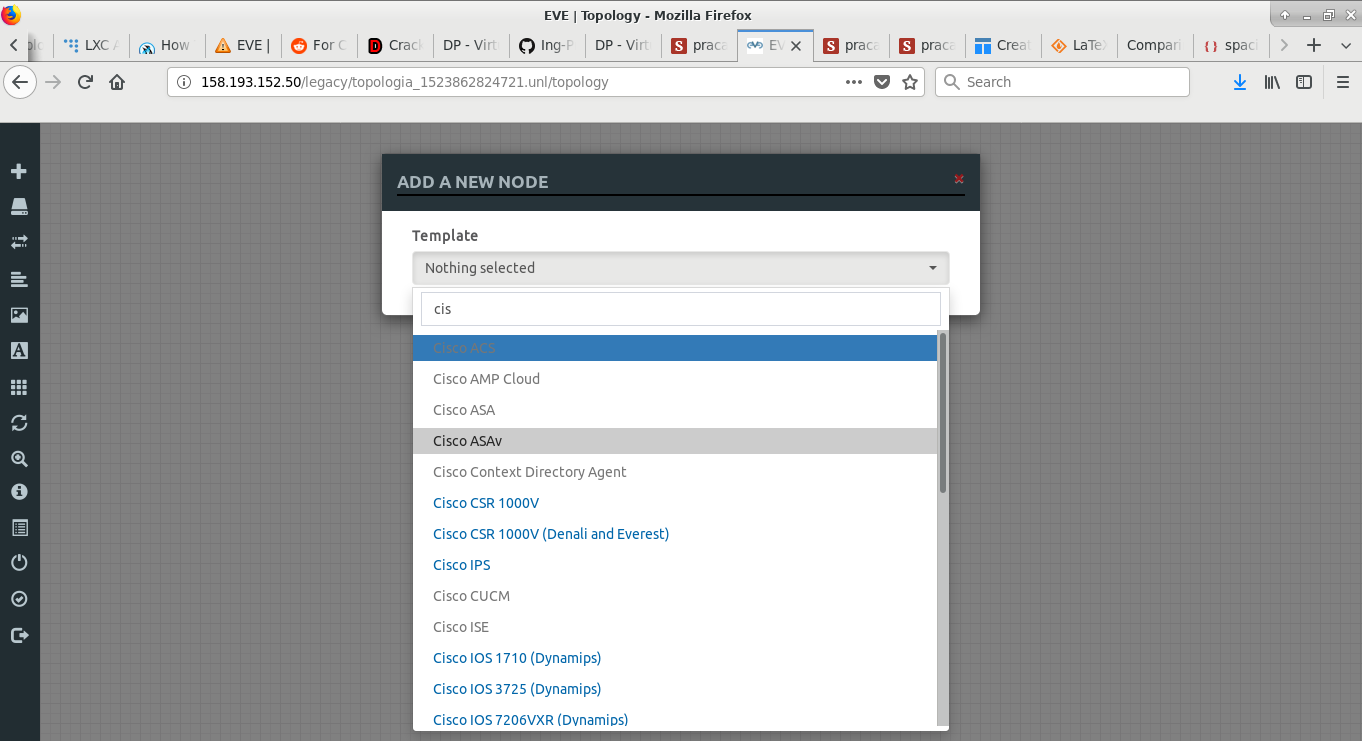
\includegraphics[width=0.65\textwidth,trim={12cm 0cm 12cm 5cm},clip]{eve_ng_add_a_new_node_selection_dialog}
    \caption{Dialógové okno pre vyhľadanie zariadenia}
    \label{obr:eve_ng_add_a_new_node_selection_dialog}
    
    \vspace{1cm}
    
    \centering
    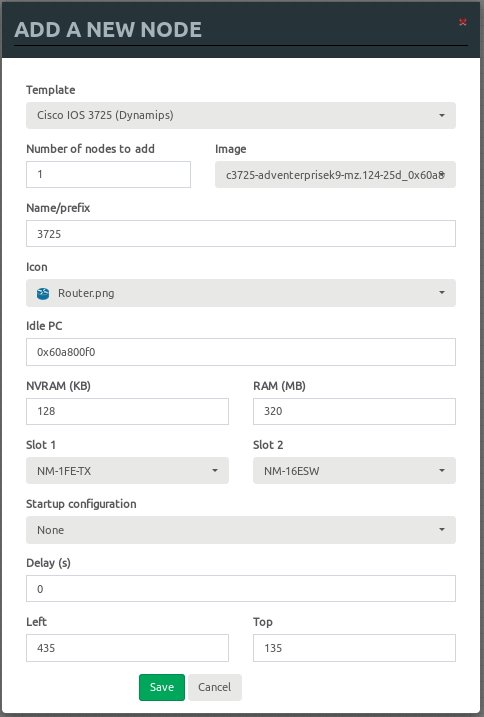
\includegraphics[width=0.5\textwidth,trim={0cm 0.1cm 0.1cm 0.1cm},clip]{eve_ng_add_a_new_node_3725_edit_dialog}
    \caption{Dialógové pre úpravu parametrov pridávaného zariadenia}
    \label{obr:eve_ng_add_a_new_node_3725_edit_dialog}
\end{figure}
    
    \item Po pridaní prvkov do topológie vytvoríme spojenia medzi jednotlivými zariadeniami. Zariadenia je možné prepájať iba rozhraniami rovnakého typu (Ethernet-Ethernet, Serial-Serial). Prepájať je možné iba \emph{vypnuté} zariadenia. Prepojenie medzi zariadeniami vytvoríme kliknutím na ikonu \emph{vidlice} s popisom \emph{Connect to another node} (obr. \ref{obr:eve_ng_prepajanie_vidlica}) a potiahnutím myši smerom ku druhému zariadeniu (obr. \ref{obr:eve_ng_prepajanie_ku_druhemu_zariadeniu}). Následne sa objaví dialógové okno s výberom rozhraní pre obidve zariadenia, ktoré majú byť prepojené (obr. \ref{obr:eve_ng_prepajanie_add_connection_dialog}). Po výbere rozhraní z oboch rozbaľovacích zoznamov klikneme na tlačidlo \emph{Save}. Dialógové okno sa zatvorí a vytvorí sa prepojenie medzi zariadeniami pre zvolené rozhrania (obr. \ref{obr:eve_ng_prepajanie_prepojenie_vytvorenie}). Po nastavení správnych IP adries na prepojených rozhraniach bude vytvorená konektivita medzi zariadeniami.
    
    \begin{comment}
    \begin{figure}
        \centering
        \includegraphics[width=0.5\textwidth,trim={8cm 15cm 30cm 7cm},clip]{eve_ng_prepajanie_vidlica}
        \caption{Ikona na prepájanie zariadení}
        \label{obr:eve_ng_prepajanie_vidlica}
        
        \centering
        \includegraphics[width=0.5\textwidth,trim={8cm 15cm 30cm 7cm},clip]{eve_ng_prepajanie_ku_druhemu_zariadeniu}
        \caption{Priebeh prepájania zariadení}
        \label{obr:eve_ng_prepajanie_ku_druhemu_zariadeniu}
    \end{figure}
    \end{comment}
    
    
    \begin{figure}
    %\centering
    \begin{minipage}{.5\textwidth}
        \centering
        \includegraphics[width=0.9\textwidth,trim={8cm 15cm 30cm 7cm},clip]{eve_ng_prepajanie_vidlica}
        \caption{Ikona na prepájanie zariadení}
        \label{obr:eve_ng_prepajanie_vidlica}
    \end{minipage}%
    \begin{minipage}{.5\textwidth}
        \centering
        \includegraphics[width=0.9\textwidth,trim={8cm 15cm 30cm 7cm},clip]{eve_ng_prepajanie_ku_druhemu_zariadeniu}
        \caption{Priebeh prepájania zariadení}
        \label{obr:eve_ng_prepajanie_ku_druhemu_zariadeniu}
    \end{minipage}
    \end{figure}
    
    
    
    
    
    \begin{figure}
        \centering
        \includegraphics[width=0.75\textwidth]{eve_ng_prepajanie_add_connection_dialog}
        \caption{Dialógové okno na výber prepájaných rozhraní}
        \label{obr:eve_ng_prepajanie_add_connection_dialog}
    \end{figure}
    
    \begin{figure}
        \centering
        \includegraphics[width=0.5\textwidth,trim={8cm 15cm 30cm 7cm},clip]{eve_ng_prepajanie_prepojenie_vytvorenie}
        \caption{Úspešné vytvorenie prepojenia}
        \label{obr:eve_ng_prepajanie_prepojenie_vytvorenie}
    \end{figure}
    
    \item Po prepojení prvkov v topológii je možné upravovať ich atribúty rôznymi spôsobmi.
    
    \begin{itemize}[noitemsep]
        \item Najjednoduchším spôsobom úpravy platným pre všetky prvky je presunutie prvku myšou.
        \item Zariadenia je možné upravovať v zozname zariadení po kliknutí na položku \emph{Nodes} v menu na ľavej strane obrazovky (obr. \ref{obr:eve_ng_configured_nodes_dialog}).
        \item Ďalší spôsob, ako upraviť parametre zariadenia je pravým kliknutím na zariadenie a kliknutím na \emph{Edit} (obr. \ref{obr:eve_ng_edit_node_dialog}).
        \item Siete sa dajú upravovať v zozname sietí po kliknutí na položku \emph{Networks} v menu na ľavej strane obrazovky (obr. \ref{obr:eve_ng_configured_networks_dialog}).
        \item Obrázky, geometrické tvary a textové polia vieme upravovať v zozname objektov po kliknutí na položku \emph{Configured objects} v menu na ľavej strane obrazovky (obr. \ref{obr:eve_ng_configured_objects_dialog}).
    \end{itemize}

\begin{figure}
    \centering
    \includegraphics[width=1\textwidth,trim={2cm 13cm 2cm 5cm},clip]{eve_ng_configured_nodes_dialog}
    \caption{Dialógové okno so zoznamom zariadení v topológii}
    \label{obr:eve_ng_configured_nodes_dialog}
\end{figure}

\begin{figure}
    \centering
    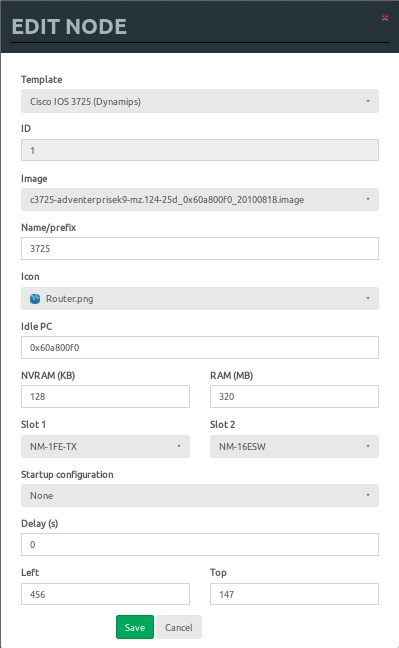
\includegraphics[width=0.6\textwidth,trim={0.1cm 0cm 0cm 0cm},clip]{eve_ng_edit_node_3725_edit_dialog}
    \caption{Dialógové okno na úpravu zariadenia}
    \label{obr:eve_ng_edit_node_dialog}
\end{figure}

\begin{figure}
    \centering
    \includegraphics[width=1\textwidth,trim={2cm 13cm 2cm 5cm},clip]{eve_ng_configured_networks_dialog}
    \caption{Dialógové okno so zoznamom sietí v topológii}
    \label{obr:eve_ng_configured_networks_dialog}
\end{figure}

\begin{figure}
    \centering
    \includegraphics[width=1\textwidth,trim={2cm 13cm 2cm 5cm},clip]{eve_ng_configured_objects_dialog}
    \caption{Dialógové okno so zoznamom grafických a textových objektov}
    \label{obr:eve_ng_configured_objects_dialog}
\end{figure}



    
Ďalší spôsob na úpravu prvkov v topológii je upravovanie samotného súboru s topológiou na serveri s príponou \emph{unl} (obr. \ref{obr:eve_ng_unl_file_syntax}). Tieto súbory sú napísané vo formáte XML a sú uložené v adresári \texttt{/opt/unetlab/labs/}. Súbory môže upravovať iba administrátor EVE-ng servera alebo používatelia so \emph{sudo} oprávneniami. Prvky sú definované značkami, ktoré definujú ich typ (zariadenie, sieť, textové pole a pod.). Nižšie je uvedený zoznam niektorých značiek použitých v \emph{unl} súbore.

    \begin{description}[noitemsep]
        \item [\texttt{<node>}] - zariadenie v topológii
        \begin{description}[noitemsep]
            \item [\texttt{id}] - identifikačné číslo zariadenia; slúži na vygenerovanie portového čísla; musí byť unikátne
            \item [\texttt{name}] - názov zariadenia; zobrazuje sa pod jeho ikonkou; malo by byť unikátne, kvôli prehľadnosti topológie
            \item [\texttt{left}] - vzdialenosť od ľavého okraja plochy v topológii
            \item [\texttt{top}] - vzdialenosť od horného okraja plochy v topológii
            \item [\texttt{uuid}] - UUID identifikátor zariadenia; musí byť unikátny; iba pre QEMU zariadenia
            \item [\texttt{firstmac}] - MAC adresa prvého rohzrania pre zariadenia; iba pre QEMU zariadenia
            \item [\texttt{<interface>}] - pripojené rozhrania pre zariadenie
            \begin{description}[noitemsep]
                \item [\texttt{id}] - identifikačné číslo pripojeného rozhrania; musí byť unikátne
                \item [\texttt{remote\_id}] - identifikačné číslo vzdialeného zariadenia - odkaz na atribúť \texttt{id} v značke \texttt{<node>} iného zariadenia; iba pre zariadenia typu IOL
                \item [\texttt{network\_id}] - identifikačné číslo siete; iba pre Ethernet rozhrania 
            \end{description}
        \end{description}
        
        \item [\texttt{<networks>}] - zoznam vytvorených sietí v topológii
        \begin{description}[noitemsep]
            \item [\texttt{<network>}] - sieť v topológii; vytvára sa ako \emph{bridge} rozhranie pre prepojenie dvoch Ethernet rozhraní medzi zariadeniami alebo pri pridaní siete z kontextového menu pri zvolení položky \emph{Network}
            \begin{description}[noitemsep]
                \item [\texttt{id}] - identifikačné číslo siete; musí byť unikátne
                \item [\texttt{visibility}] - viditeľnosť siete; v prípade, že prepájame dve Ethernet rohrania, je atribút nastavený na hodnotu 0 - sieť (bridge rozhranie) je v topológii skrytá; ak pridávame do topológie sieť explicitne cez \emph{Add a new object} -> \emph{Network}, atribút sa nastaví na hodnotu 1 a sieť bude viditeľná v topológii
            \end{description}
        \end{description}
    \end{description}

Zmeny v \emph{unl} súbore sa prejavia až po znovunačítaní stránky (klávesou F5) alebo topológie (kliknutím na \emph{Refresh topology} v menu na ľavej strane obrazovky).

\begin{figure}
    \centering
    \includegraphics[width=0.75\textwidth,trim={0cm 0cm 0cm 1.9cm},clip]{eve_ng_unl_file_syntax}
    \caption{Ukážka UNL súboru}
    \label{obr:eve_ng_unl_file_syntax}
\end{figure}
    
Experimentovaním sme zistili, že vytváranie topológii a duplikácia jej prvkov v \emph{unl} súbore je pomerne náročná, zdĺhavá a náchylná na chyby. Pri duplikácii zariadení bolo náročné udržať prehľad o.i. aj o identifikátoroch zariadení a rozhraní a ich vzájomnom prepojení. Výhodnejšie sa ukázalo najprv použiť webové rozhranie, potom tabuľku zariadení \emph{Nodes} a nakoniec upraviť \emph{unl} súbor:
    
    \begin{enumerate}[noitemsep]
        \item Najpr vo webovom rozhraní vytvoríme topológiu, pridáme do nej zariadenia a poprepájame ich.
        \item Potom v tabuľke zariadení \emph{Nodes} upravíme názvy zariadení v stĺpci \emph{Name} (obr. \ref{obr:eve_ng_configured_nodes_dialog}).
        \item Ak je potrebné, nakoniec v \emph{unl} súbore presnejšie upravíme súradnice prvkov v topológii definovaných atribútmi \texttt{left} a \texttt{top}. Výsledkom týchto úprav je celkové zlepšenie vzhľadu topológie. Môžeme tak urobiť aj vo webovom rozhraní v dialógovom okne pre úpravu zariadenia v atribútoch \emph{Left} a \emph{Top}, avšak v \emph{unl} súbore vieme súradnice prvkov upraviť hromadne.
    \end{enumerate}
    
    \item Potom, ako sme pridali zariadenia do topológie a navzájom ich prepojili, ich môžeme spustiť. Zariadenia sa dajú spustiť buď jednotlivo, skupinovo alebo všetky naraz. Zariadenia môže spúšťať iba používateľ s rolou \emph{admin} alebo \emph{editor}.

    \begin{itemize}[noitemsep]
        \item Jedno zariadenie spustíme tak, že naň klikneme pravým tlačidlom a zvolíme \emph{Start} (obr. \ref{obr:eve_ng_spustanie_po_jednom_context_menu}).
        \item Skupinu zariadení spustíme tak, že ich najpr označíme myšou resp. vyberieme zariadenia kombináciou \emph{Ctrl + ľavé kliknutie}. Následne na jedno z označených zariadení klikneme pravým tlačidlom a zvolíme \emph{Start Selected} (obr. \ref{obr:eve_ng_spustanie_skupiny_context_menu}).
        \item Všetky zariadenia spustíme kliknutím na položku \emph{More actions} a zvolíme možnosť \emph{Start all nodes} (obr. \ref{obr:eve_ng_spustanie_vsetkych_context_menu}).
    \end{itemize}

\begin{comment}
\begin{figure}
    \centering
    \includegraphics[width=0.3\textwidth,trim={11cm 5cm 28cm 9cm},clip]{eve_ng_spustanie_po_jednom_context_menu}
    \caption{Spustenie jedného zariadenia}
    \label{obr:eve_ng_spustanie_po_jednom_context_menu}
\end{figure}

\begin{figure}
    \centering
    \includegraphics[width=0.4\textwidth,trim={11cm 3cm 19cm 9cm},clip]{eve_ng_spustanie_skupiny_context_menu}
    \caption{Spustenie skupiny zariadení}
    \label{obr:eve_ng_spustanie_skupiny_context_menu}
\end{figure}
\end{comment}

\begin{figure}
%\centering
\begin{minipage}{.4\textwidth}
    \vspace{1.1cm}
    \centering
    \includegraphics[width=0.8\textwidth,trim={11cm 5cm 27cm 9cm},clip]{eve_ng_spustanie_po_jednom_context_menu}
    \caption{Spustenie jedného zariadenia}
\label{obr:eve_ng_spustanie_po_jednom_context_menu}
\end{minipage}%
\begin{minipage}{.6\textwidth}
    \centering
    \includegraphics[width=1\textwidth,trim={11cm 3cm 19cm 9cm},clip]{eve_ng_spustanie_skupiny_context_menu}
    \caption{Spustenie skupiny zariadení}
    \label{obr:eve_ng_spustanie_skupiny_context_menu}
\end{minipage}
\end{figure}

\begin{figure}
    \centering
    \includegraphics[width=0.6\textwidth,trim={0cm 3cm 29cm 9cm},clip]{eve_ng_spustanie_vsetkych_sidemenu}
    \caption{Spustenie všetkých zariadení}
    \label{obr:eve_ng_spustanie_vsetkych_context_menu}
\end{figure}
      
    \item \label{item:vzdialeny_pristup} Po spustení zariadení sa sprístupní ich vzdialená konzola. Spôsob, akým sa na pripájame na konzoly zariadení sa líši podľa toho, v akom móde sme sa do EVE-ng prihlásili. V bode \ref{item:prihlasenie} sme spomenuli, že do webového rozhrania EVE-ng sa dá prihlásiť v dvoch režimoch: v HTML5 alebo natívnom móde. Výber módu priamo ovplyvňuje aj spôsob, akým pristupujeme ku konzolám zariadení.
    
    HTML5 mód zabezpečuje vzdialený prístup k zariadeniam pomocou reverzného proxy servera \emph{Apache Guacamole}, ktorý sa pripája na konzoly zariadení. V tomto móde sa na obrazovke s otvorenou topológiou po kliknutí na zariadenie otvorí jeho vzdialená konzola, pričom nie je možné pripojiť sa ku konzolám zariadenia pomocou telnet alebo vnc klienta. HTML5 mód web rozhrania EVE-ng bol však menej stabilný a reagoval výrazne pomalšie pri práci s topológiou v provonaní s natívnym módom. Preto bolo webové rozhranie ďalej používané iba v natívnom režime.
        
    Natívny režim vyžaduje, aby sme mali pre vzdialený prístup ku zariadeniam na lokálnom počítači nainštalované dodatočné nástroje. 
        
    Na prístup k zariadeniam z lokálneho počítača potrebujeme mať nainštalovaného telnet a VNC klienta. Pre platformu Windows môžeme zvoliť kombináciu napr. \emph{PuTTY} a \emph{RealVNC Viewer}, pre platformu Linux zase terminál, napr. \emph{BASH} a \emph{TigerVNC}. Následne sa navigujeme myšou na zariadenie, na ktoré sa chceme pripojiť, ale namiesto toho, aby sme naň klikli, zapamätáme si údaje zobrazené v ľavom alebo pravom dolnom rohu obrazovky (obr. \ref{obr:eve_ng_protokol_ip_port}) t.j. protokol, IP adresa servera a portové číslo. Tieto údaje následne zadáme do zodpovedajúceho klienta podľa protokolu. Po zadaní správnych údajov by sme sa mali pripojiť na vzdialenú konzolu zariadenia.

\begin{figure}
    \centering
    \includegraphics[width=0.6\textwidth,trim={0cm 0cm 0.8cm 4cm},clip]{eve_ng_protokol_ip_port}
    \caption{Adresa na vzdialený prístup k zariadeniu (vľavo dole)}
    \label{obr:eve_ng_protokol_ip_port}
\end{figure}

    Aby sme mohli pristupovať ku konzole zariadenia z webového rozhrania pri kliknutí naň, potrebujeme mať na lokálnom počítači nainštalovaný tzv. EVE-ng integračný balíček. Ten existuje pre platformy Windows a Linux. Ďalej sme upravovali iba integračný balíček pre platformu Linux, z ktorého nakoniec vznikla ďalšia, bezpečnejšia verzia. Jednalo sa úpravy, ktoré zabezpečovali vzdialený prístup k zariadeniam s protokolmi \emph{telnet} a \emph{vnc} pomocou SSH tunelov a odchytávanie prevádzky z rozhrania zariadenia ako štandardný používateľ namiesto používateľa \emph{root}. Predvolený integračný baliček takéto funkciu neobsahuje. Vykonané úpravy nemajú výrazný vplyv na funkcionalitu pre koncového používateľa.
    
    Predvolené verzie integračných balíčkov je možné stiahnuť zo zdroja \cite{eve_ng_integration_pack_win} pre platformu Windows a zo zdroja \cite{eve_ng_integration_pack_linux} pre platformu Linux. Inštalácia a popis jednotlivých úprav integračného balíčka EVE-ng pre platformy Windows a Linux je popísaná v kapitole \ref{chap:cd} v bode \ref{item:integracia_s_prehliadacmi} Upravená verzia integračného balíčka pre platformu Linux je dostupná v kapitole \ref{chap:cd} v bode \ref{item:upraveny_integracny_balicek_win}

\end{enumerate}

Vyššie uvedené kroky popisujú vytvorenie základnej topológie s rôznymi prvkami. V ďalších častiach bude popísané, ako EVE-ng generuje a priďeľuje portové čísla zariadeniam, pomocou ktorých sa pripájame na ich vzdialené konzoly a to, ako prepojiť viacero topológii medzi sebou resp. ako pripojiť topológiu k internetu.




\subsection{Prideľovanie portových čísel zariadeniam}
\label{chap:priradovanie_portovych_cisel}

Po pridaní ľubovoľného zariadenia do topológie sa preň vygeneruje portové číslo, ktoré mu je následne priradené. Portové čísla rozlišujú zariadenia v topológii a  slúžia na pripojenie sa na ich vzdialené konzoly. Vždy sa vyberie najnižšie dostupné portové číslo.

Rozsah portových čísel pre daného používateľa sa generujú vzťahom \emph{32768 + 128 * POD + ID}, kde \emph{POD} je unikátne identifikačné číslo používateľa a \emph{ID} je unikátne identifikačné číslo zariadenia. Za uvedený výpočet je zodpovená funkcia \texttt{\_\_construct} v súbore \\ \emph{/opt/unetlab/html/includes/\_\_node.php}.

Ak do topológie pridáme viacero zariadení naraz, budú mať portové čísla idúce za sebou.

V prípade, že si rôzni používatelia otvoria rovnaký súbor s topológiou, bude mať každý z používateľov prístup ku vlastným zariadeniam. Pokiaľ bude počet zariadení v topológii <= 63, portové čísla zariadení sa nebudú prekrývať a každý z používateľov bude môcť pracovať s topológiou nezávisle na sebe. Ak ľubovoľný z používateľov do topológie pridá zariadenie, uvidia ho všetci, ale až po obnovení topológie (F5/\emph{Refresh topology}).

Vyššie uvedené správanie bolo otestované po otvorení rovnakého súboru s topológiou dvomi rôznymi používateľmi s rôznymi používateľskými rolami (\emph{admin} a \emph{editor}).

S prideľovaním portových čísel súvisí aj problém popísaný v časti \ref{chap:zatvorenie_topo_so_spustenymi_zariadeniami}, pretože do vzťahu na výpočet portového čísla sa neberie do úvahy počet topológii, ktoré má používateľ spustené.

%Na obr. \ref{obr:eve_ng_rovnaka_topo_prvy_pouzivatel_admin} vidíme, že prvý používateľ už má spustené zariadenia, ale druhý používateľ ich ako spustené nevidí (obr. \ref{obr:eve_ng_rovnaka_topo_druhy_pouzivatel_editor}).

\begin{comment}
\begin{figure}
    \centering
    \includegraphics[width=0.75\textwidth,trim={0cm 0cm 0cm 4cm},clip]{eve_ng_rovnaka_topo_prvy_pouzivatel_admin}
    \caption{Topológia prvého používateľa s používateľskou rolou \emph{admin}}
    \label{obr:eve_ng_rovnaka_topo_prvy_pouzivatel_admin}
\end{figure}

\begin{figure}
    \centering
    \includegraphics[width=0.75\textwidth,trim={0cm 0cm 0cm 4cm},clip]{eve_ng_rovnaka_topo_druhy_pouzivatel_editor}
    \caption{Topológia druhého používateľa s používateľskou rolou \emph{editor}}
    \label{obr:eve_ng_rovnaka_topo_druhy_pouzivatel_editor}
\end{figure}
\end{comment}



\subsection{Pripojenie topológie k internetu / prepojenie topológii navzájom}

Do EVE-ng topológie je možné pridať prvok typu \emph{sieť}, ktorý umožňuje prepájať topológie medzi sebou alebo ich pripájať ku internetu.

Sieť do topológie pridáme kliknutím na ikonu \textbf{+} (\emph{Add an object}) a zo zoznamu vybierieme položku \emph{Network}. Objaví sa dialógové okno na úpravu parametrov pridávanej siete (obr. \ref{obr:eve_ng_add_network_dialog}). Pre správnu funkčnosť a prehľadnosť stačí zmeniť iba atribúty \emph{Name} a \emph{Type}. To textového poľa atribútu \emph{Name} zadáme názov pridávanej siete. Z rozbaľovacieho zoznamu (obr. \ref{obr:eve_ng_add_network_dialog_network_types}) si následne zvolíme typ siete:

\begin{figure}
    \centering
    \includegraphics[width=0.75\textwidth,trim={13cm 7cm 13cm 5.2cm},clip]{eve_ng_add_network_dialog}
    \caption{Dialógové okno pre pridanie siete}
    \label{obr:eve_ng_add_network_dialog}
\end{figure}

\begin{description}
    \item [bridge] - Slúži na vytvorenie siete na prepojenie zariadení v jednej topológii.
    \item [Management (Cloud0)] - Sieť, pomocou ktorj vieme pripojiť topológiu k živej sieti alebo internetu.
    \item [Cloud1-9] - Siete, ktoré slúžia na prepájanie topológii medzi sebou na jednom serveri.
\end{description}

\begin{figure}
    \centering
    \includegraphics[width=0.3\textwidth,trim={0cm 0cm 0.3cm 0cm},clip]{eve_ng_add_network_dialog_network_types}
    \caption{Typy sietí}
    \label{obr:eve_ng_add_network_dialog_network_types}
\end{figure}

Po pridaní siete do topológie k nej môžeme pripájať ľubovoľný počet zariadení prostredníctvom Ethernet rozhraní. Sieť bude pre zariadenia, ktoré sú na ňu pripojené, slúžiť ako \emph{hub (rozbočovač)}, čím je možné v topológiách vytvárať \emph{broadcast} domény.

V prípade, že topológiu pripájame na živú sieť prostredníctvom \emph{Cloud0}, je potrebné pre rozhranie zariadenia pripojeného k tejto sieti priradiť IP adresu buď pomocou DHCP, alebo staticky manuálnou konfiguráciou. Ak je potrebné, povolíme IP adresu na zariadení \emph{firewall}. Príklad topológie s rôznymi typmi sietí je znázornený na obr. \ref{obr:eve_ng_siete_v_topologii}.

\begin{figure}
    \centering
    \includegraphics[width=1\textwidth,trim={9cm 7cm 12.5cm 4cm},clip]{eve_ng_siete_v_topologii}
    \caption{Ukážka topológie s rôznymi typmi sietí}
    \label{obr:eve_ng_siete_v_topologii}
\end{figure}

%%%%%%%%%%%%%%%%%% literatura

\begin{thebibliography}{99}
\label{literatura}
\addcontentsline{toc}{chapter}{Literatúra}

\bibitem{hvlab}
HWANG Wu-Yuin, HAREGOT Michaele, KONGCHAROEN Chaknarin (2017) {\it Web-based hybrid virtualization laboratory to facilitate network learning: HVLab}. IEEE Conference Publication. ISBN: 978-1-5386-1431-0

\bibitem{opennebula_lab}
Yu.A. USHAKOV, P.N. POLEZHAEV, L.V. LEGASHEV, A.E. SHUKHMAN, I.P. BOLODURINA (2016) {\it  Virtual cloud network laboratory based on IaaS with automatized creation of network topology on demand }. IEEE Conference Publication. ISBN: 978-1-5090-1841-3

\bibitem{packet_tracer}
Cisco Systems, Inc. (03-26-2018) {\it Introduction to Packet Tracer | Cisco NetAcad}. [Online] [cit. 2018-03-27]. \\ 
Dostupné na: <\url{https://www.netacad.com/courses/intro-packet-tracer/}>.

\bibitem{packet_tracer_mac}
MCKENZIE Peter (10-17-2016) {\it Where to find packet tracer for Mac OS? How to install it? - 101872 - The Cisco Learning Network}. [Online] [cit. 2018-03-27]. \\
Dostupné na: <\url{https://learningnetwork.cisco.com/thread/101872}>.

\bibitem{obr_packet_tracer}
ccnav6.com (07-05-2017) {\it 7.1.1.4 Packet Tracer - ACL Demonstration Instructions Answers}. [Online] [cit. 2018-03-25]. \\ 
Dostupné na: <\url{https://ccnav6.com/wp-content/uploads/2017/07/7.1.1.4-Packet-Tracer-ACL-Demonstration-Instructions.jpg}>.

\bibitem{dynamips}
EasyPass Computer Training Centre (05-08-2016) {\it Dynamips / Dynagen Tutorial}. [Online] [cit. 2018-03-25]. \\ 
Dostupné na: <\url{http://www.iteasypass.com/Dynamips.htm}>.

\bibitem{obr_dynamips_dynagen}
EasyPass Computer Training Centre (05-08-2016) {\it Dynamips / Dynagen Tutorial}. [Online] [cit. 2018-03-25]. \\ 
Dostupné na: <\url{http://www.iteasypass.com/Dynamips\%20-\%20Dynagen\%20Tutorial.files/image002.gif}>

\bibitem{dynamips_github}
DUPONCHELLE Julien, LINTOTT Daniel, GROSSMANN Jeremy (07-24-2017) {\it GNS3/dynamips: Dynamips development}. [Online] [cit. 2018-03-25]. \\ 
Dostupné na: <\url{https://github.com/GNS3/dynamips}>.

\bibitem{dynamips_nil}
SEGEČ Pavel, NIL - Network Information Library (04-11-2014) {\it Connecting Dynamips/Dynagen router with a real network - in linux | NIL - Network Information Library}. [Online] [cit. 2018-03-25]. \\ 
Dostupné na: <\url{http://nil.uniza.sk/network-simulation-and-modelling/dynamipsdynagen/connecting-dynamipsdynagen-router-real-network-linux}>.

\bibitem{webiou_unetlab_unetlabv2}
Route Reflector Labs (03-21-2018) {\it Unified Networking Lab v2 (UNetLabv2) | Andrea Dainese}. [Online] [cit. 2018-03-25]. \\
Dostupné na: <\url{http://www.routereflector.com/unetlab/}>.

\bibitem{webiou_github}
DAINESE Andrea (05-30-2016) {\it dainok/iou-web}. [Online] [cit. 2018-03-25]. \\
Dostupné na: <\url{https://github.com/dainok/iou-web}>.

\bibitem{webiou_firewall_cx}
WANG Jack (2017) {\it Cisco IOU}. [Online] [cit. 2018-03-25]. \\
Dostupné na: \\
\href{http://www.firewall.cx/cisco-technical-knowledgebase/cisco-services-tech/1172-cisco-virl-virtual-internet-routing-lab-introduction.html}{<\texttt{http://www.firewall.cx/cisco-technical-knowledgebase/cisco-services-\\tech/1172-cisco-virl-virtual-internet-routing-lab-introduction.html}>}.

\bibitem{webiou_80211}
FORDHAM Stuart (06-15-2013) {\it Getting started with Cisco IOU - IOS on Unix - Part 1 | www.802101.com}. [Online] [cit. 2018-03-25]. \\
Dostupné na: \\
<\url{https://www.802101.com/getting-started-cisco-iou-ios-unix/}>.

\bibitem{webiou_real_network}
FERRO Greg (04-17-2011) {\it Cisco IOU:Connect IOU with real or external networks — EtherealMind}. [Online] [cit. 2018-03-25]. \\
Dostupné na: \\<\url{http://etherealmind.com/cisco-iou-external-real-network-remote/}>.

\bibitem{obr_webiou}
FARES Ryan (12-10-2015) {\it Cisco IOU Web Interface – netbrainstlearn}. [Online] [cit. 2018-03-25]. \\
Dostupné na: \\
<\url{https://i2.wp.com/www.routereflector.com/images/posts/2012/09/iou-web-new.png}>.

\bibitem{virl_cisco}
Cisco Systems, Inc. (2018) {\it Cisco Virtual Internet Routing Lab Personal Edition (VIRL PE) 20 Nodes - The Cisco Learning Network}. [Online] [cit. 2018-03-26]. \\
Dostupné na: \\
\href{https://learningnetworkstore.cisco.com/virtual-internet-routing-lab-virl/cisco-personal-edition-pe-20-nodes-virl-20}{<\texttt{https://learningnetworkstore.cisco.com/virtual-internet-routing-lab\\-virl/cisco-personal-edition-pe-20-nodes-virl-20}>}.

\bibitem{virl_interfacett_1}
JACOB Mark, Interface Technical Training (08-14-2015) {\it How to create a simple network topology using Cisco VIRL}. [Online] [cit. 2018-03-26]. \\
Dostupné na: \\
\href{https://www.interfacett.com/blogs/how-to-create-a-simple-network-topology-using-ciscos-virl/}{<\texttt{https://www.interfacett.com/blogs/how-to-create-a-simple-network\\-topology-using-ciscos-virl/}>}.

\bibitem{virl_interfacett_2}
JACOB Mark, Interface Technical Training (08-28-2015) {\it How to interact with a simple network topology built using Cisco’s VIRL}. [Online] [cit. 2018-03-26]. \\
Dostupné na: \\
\href{https://www.interfacett.com/blogs/how-to-interact-with-a-simple-network-topology-built-using-ciscos-virl/}{<\texttt{https://www.interfacett.com/blogs/how-to-interact-with-a-simple\\-network-topology-built-using-ciscos-virl/}>}.

\bibitem{virl_ciscoskills}
Cisco Skills (01-07-2017) {\it Cisco VIRL and Windows VMs}. [Online] [cit. 2018-03-26]. \\
Dostupné na: \\<\url{https://ciscoskills.net/2017/01/07/cisco-virl-and-windows-vms/}>.

\bibitem{virl_speaknetworks}
WANG Jack (07-27-2015) {\it Cisco VIRL External Connectivity – Speak Network Solutions}. [Online] [cit. 2018-03-26]. \\
Dostupné na: \\<\url{https://www.speaknetworks.com/cisco-virl-external-connectivity/}>.

\bibitem{virl_cisco_features}
Cisco Systems, Inc. (2018) {\it Virtual Internet Routing Lab (VIRL) Features - The Cisco Learning Network Store}. [Online] [cit. 2018-03-26]. \\
Dostupné na: <\url{https://learningnetworkstore.cisco.com/virlfaq/features}>.

\bibitem{virl_edition_differences}
LIU Wen, Inc. (04-28-2016) {\it VIRL Personal Edition vs. the Academic Edition - 30411 - The Cisco Learning Network}. [Online] [cit. 2018-03-26]. \\
Dostupné na: <\url{https://learningnetwork.cisco.com/docs/DOC-30411}>.

\bibitem{obr_virl_vmmaestro}
JACOB Mark, Interface Technical Training (08-28-2015) {\it How to interact with a simple network topology built using Cisco’s VIRL}. [Online] [cit. 2018-03-26]. \\
Dostupné na: \\
<\url{https://www.interfacett.com/wp-content/uploads/2015/08/013-interact-with-simple-network-topology-in-Cisco-VIRL.jpg}>.

\bibitem{obr_virl_web}
JACOB Mark, Interface Technical Training (08-28-2015) {\it How to interact with a simple network topology built using Cisco’s VIRL}. [Online] [cit. 2018-03-26]. \\
Dostupné na: \\
<\url{https://www.interfacett.com/wp-content/uploads/2015/08/013-interact-with-simple-network-topology-in-Cisco-VIRL.jpg}>.

\bibitem{incapsula_cms}
CASSETTO Orion (09-26-2017) {\it Why CMS Platforms Are Common Hacking Targets | Security Tips}. [Online] [cit. 2018-04-13]. \\
Dostupné na: \\
<\url{https://www.incapsula.com/blog/cms-security-tips.html}>.

\bibitem{viro_hadac}
HADAČ Peter (04-27-2017) {\it ViRo2 - online web nástroj na podporu vyučovania sietí}. [Online] [cit. 2018-03-26] str. 32-36, 52-55. \\
Dostupné na: \\
<\url{http://opac.crzp.sk/?fn=detailBiblioForm&sid=F972C28947B4ECBEDC061D4570AC&seo=CRZP-detail-kniha}>.

\bibitem{stackoverflow_survey}
Stack Exchange Inc (2018-03-19) {\it Stack Overflow Developer Survey 2018}. [Online] [cit. 2018-03-27] \\
Dostupné na: \\
<\url{https://insights.stackoverflow.com/survey/2018/?utm_source=Iterable&utm_medium=email&utm_campaign=dev-survey-2018-promotion#most-loved-dreaded-and-wanted}>.

\bibitem{unetlab_github}
DAINESE Andrea (05-23-2017) {\it dainok/iou-web}. [Online] [cit. 2018-03-26]. \\
Dostupné na: <\url{https://github.com/dainok/iou-web}>.

\bibitem{obr_unetlab_web}
HAGEN, LAN-Monitor.de  (03-19-2016) {\it Was ist UNetLab? – LAN-Monitor.de}. [Online] [cit. 2018-03-26]. \\
Dostupné na: \\
<\url{https://www.lan-monitor.de/wp-content/uploads/was-ist-unetlab-01-test-lab.png}>.

\bibitem{obr_unetlabv2_arch}
DAINESE Andrea, Route Reflector Labs (03-21-2018) {\it Unified Networking Lab v2 (UNetLabv2) | Andrea Dainese}. [Online] [cit. 2018-03-26]. \\
Dostupné na: \\
<\url{http://www.routereflector.com/images/unetlab/unetlab-architecture.png}>.

\bibitem{eve_ng_technologies}
BuiltWith® Pty Ltd (03-26-2018) {\it IP\_adresa\_servera Technology Profile}. [Online] [cit. 2018-03-26]. \\
Dostupné na: <\url{https://builtwith.com/IP\_adresa\_servera}>.

\bibitem{eve_ng_versions_table}
EVE-NG Ltd. (2018) {\it Compare Editions}. [Online] [cit. 2018-03-26]. \\
Dostupné na: <\url{http://www.eve-ng.net/index.php/features/compare}>.

\bibitem{eve_ng_versions_list}
EVE-NG Ltd. (2018) {\it Features}. [Online] [cit. 2018-03-26]. \\
Dostupné na: <\url{http://www.eve-ng.net/index.php/features/features}>.

\bibitem{gns3_docker}
ZIAJKA Dominik, GROSSMANN Jeremy, DUPONCHELLE Julien (02-08-2018) {\it Docker support in GNS3 - GNS3}. [Online] [cit. 2018-03-26]. \\
Dostupné na: \\
<\url{https://docs.gns3.com/1KGkv1Vm5EgeDusk1qS1svacpuQ1ZUQSVK3XqJ01WKGc/}>.

\bibitem{gns3_gui_github}
ZIAJKA Dominik, GROSSMANN Jeremy (03-12-2018) {\it GNS3/gns3-gui: GNS3 Graphical Network Simulator: GNS3 server}. [Online] [cit. 2018-03-27]. \\
Dostupné na: <\url{https://github.com/GNS3/gns3-gui}>.

\bibitem{gns3_server_github}
ZIAJKA Dominik, GROSSMANN Jeremy (03-14-2018) {\it GNS3/gns3-server: GNS3 server}. [Online] [cit. 2018-03-27]. \\
Dostupné na: <\url{https://github.com/GNS3/gns3-server}>.

\bibitem{gns3_web_github}
ZIAJKA Dominik (03-26-2018) {\it GNS3/gns3-web-ui: WebUI implementation for GNS3}. [Online] [cit. 2018-03-27]. \\
Dostupné na: <\url{https://github.com/GNS3/gns3-web-ui}>.

\bibitem{gns3_console_ports}
ZUPPETTA Bruno Paolo (September 2017) {\it Discussions - Console port - GNS3}. [Online] [cit. 2018-03-27]. \\
Dostupné na: <\url{https://www.gns3.com/qa/console-port-2}>.

\bibitem{gns3_console_ports_remote}
LOOKY Silva (06-05-2017) {\it Discussions - Edit the default "Console Port Range" for remote server ? - GNS3}. [Online] [cit. 2018-03-27]. \\
Dostupné na: \\
<\url{https://www.gns3.com/discussions/edit-the-default-console-port-ra}>.

\bibitem{nested_virtualization}
VMware, Inc. (03-11-2016) {\it GNS3/gns3-server: GNS3 server}. [Online] [cit. 2018-03-27]. \\
Dostupné na: <\url{https://communities.vmware.com/docs/DOC-8970}>.

\bibitem{ccna_security_topics}
Cisco Systems, Inc. (02-07-2018) {\it IINS Exam Topics - The Cisco Learning Network}. [Online] [cit. 2018-03-31]. \\
Dostupné na: \\
<\url{https://learningnetwork.cisco.com/community/certifications/security_ccna/iins-v3/exam-topics}>.

\bibitem{eve_ng_howtos}
EVE-NG Ltd. (04-01-2018) {\it HowTo's}. [Online] [cit. 2018-04-01]. \\
Dostupné na: <\url{http://www.eve-ng.net/index.php/documentation/howto-s/}>.

\bibitem{eve_ng_faq}
EVE-NG Ltd. (03-31-2018) {\it FAQ}. [Online] [cit. 2018-04-03]. \\
Dostupné na: <\url{http://www.eve-ng.net/index.php/faq}>.

\bibitem{eve_ng_integration_pack_win}
EVE-NG Ltd. {\it Windows Client side Pack}. [Online] [cit. 2018-04-16]. \\
Dostupné na: \\
<\url{http://www.eve-ng.net/downloads/windows-client-side-pack}>.

\bibitem{eve_ng_integration_pack_linux}
EVE-NG Ltd. {\it Linux Client side Pack}. [Online] [cit. 2018-04-16]. \\
Dostupné na: <\url{http://www.eve-ng.net/downloads/linux-client-side}>.

\bibitem{mpls_zakladna_topo}
SEGEČ Pavel {\it Projektovanie sietí 1, Prednáška - MPLS}. [Online] [cit. 2018-04-19]. \\
Dostupné na:\\
\href{https://github.com/kyberdrb/FRI/raw/master/Ing/2.semester/Projektovanie_Sieti_1/cvika/cv10_11_MPLS/dokumentacia_MPLS/obr/mpls_isis_topo.png}{<\texttt{https://github.com/kyberdrb/FRI/raw/master/Ing/2.semester/\\Projektovanie\_Sieti\_1/cvika/cv10\_11\_MPLS/dokumentacia\_MPLS/\\
obr/mpls\_isis\_topo.png}>}.

\bibitem{dalsie_navody_eve_ng}
{\it Unetlab Installation on ESXi | Nbctcp's Weblog}. [Online] [cit. 2018-04-19]. \\
Dostupné na:\\
\href{https://nbctcp.wordpress.com/2015/07/02/unetlab-installation-on-esxi/}{<\texttt{https://nbctcp.wordpress.com/2015/07/02/unetlab-installation-on-esxi/}>}.

\bibitem{eve_ng_qemu_namings}
EVE-NG Ltd. {\it Qemu image naming}. [Online] [cit. 2018-04-19]. \\
Dostupné na: <\url{http://www.eve-ng.net/documentation/images-table}>.

\end{thebibliography}	%  Literatura

\end{document}


